
\section{Introduction}
In numerical algebraic geometry, curve tracking algorithms were originally introduced for solving polynomial systems using homotopy continuation, see, e.g., \cite{Sommese:2005,Bertini:2013} and the references therein.  More recently, the study of the connectivity structure defined by homotopy paths has opened new avenues of research, e.g., \cite{Sommese:2001,GaloisDuff:2022}.  With the recent development of efficient certified homotopy continuation methods in \cite{xu2018approach,guillemot2024validated,duff2024certified}, the computations of these connectivity structures become proofs.  The current paper continues this approach, using homotopy continuation and interval arithmetic to produce certified approximations to curves in arbitrary dimensions as well as their generic projections to $\mathbb{R}^2$.

Suppose $C$ is a smooth algebraic curve without self-intersections in $\mathbb{R}^n$ for some $n\geq 3$ and $x\in\mathbb{R}^n$ approximates a point $x^\star$ on the curve.  We present two certified algorithms for computations with this curve.  First, we provide an algorithm to compute an isotopic approximation to the component of the curve $C$ which contains $x^\star$ along with a tubular neighborhood containing this component of the curve $C$.  Second, if $\pi:\mathbb{R}^n\rightarrow\mathbb{R}^2$ is a generic projection, then we compute an isotopic approximation to the image of the component of the curve $C$ which contains $x^\star$ under the projection $\pi$.  In our calculations, the curve $C$ is usually given implicitly as the zero set of a system of $n-1$ polynomials, but our approach also applies to open curves given parametrically by $x=\gamma(t)$, where $\gamma$ consists of $n$ univariate polynomials.

For our first algorithm, we combine and develop ideas from the certified homotopy continuation algorithms \cite{guillemot2024validated,duff2024certified} with the certified curve tracking algorithm \cite{martin2013certified}.  This results in a certified approximation to the curve which can be locally refined as needed.  We note that one of the significant differences between our approach and that of \cite{martin2013certified} is that we do not use a global upper bound on the allowed step-size, and our algorithm is guaranteed to terminate with correct output on all nonsingular curves.

In our second algorithm, we introduce ideas from \cite{Byrd:2023} to correctly approximate intersections in the image of the curve after a generic projection to $\mathbb{R}^2$.  We observe that, due to a dimension argument, a generic projection $\pi:\mathbb{R}^n\rightarrow\mathbb{R}^m$ with $m>2$ introduces no intersections.  On the other hand, projections to $\mathbb{R}^2$ typically introduce intersections.  These intersections induce the main challenge in the construction of an approximation.  In particular, the issue is that the projection of an approximation may not be an approximation of the projection as errors in the approximation may introduce or miss self-intersections.

\subsection*{Outline}

In Section \ref{sec:background}, we review the necessary background for the paper from the certified computation literature.  In Section \ref{sec:path_tracking_algorithm}, we present the path tracking algorithm under study in this paper, see Algorithm \ref{algo:certified_curve_tracking}.  We apply this algorithm in Section \ref{sec:approximation} to develop Algorithm \ref{algo:certified_plane_curve}, which computes certified approximations to generic projections of curves.  Finally, a GitHub repository holds the code used to construct the illustrative examples (\Cref{fig:tubular_nbd,fig:two_projections,fig:PTOPO_example}) in this paper at

\centerline{\url{https://github.com/klee669/certified_curve_projections}}

\section{Background}\label{sec:background}
Suppose that $C$ is a smooth algebraic curve without self-intersections in $\mathbb{R}^n$ given by the common zeros of a polynomial system $F$ consisting of $n-1$ polynomials in $n$ variables.  Here, smooth means that the derivative of $C$ is nonzero everywhere, and we also observe that the self-intersection restriction does not exclude closed curves.  The algorithms in this paper compute certified piecewise-linear approximations to the curve $C$ and its generic projections.  In this context, a certified algorithm is one that provides a proof of correctness for its output, and, for our problems, the output is correct if the approximation and curve are close in Hausdorff distance and there is an ambient isotopy deforming the curve to the approximation.  In all of our algorithms we consider polynomial systems and inputs with coefficients in $\mathbb{Q}$ because they can be represented exactly on a computer and to avoid having to address how arbitrary real numbers are represented.

There is an extensive history of curve tracking algorithms, but there are relatively fewer certified path tracking algorithms, see, e.g., \cite{kearfott1994interval,Kim:2004,PV:2004,PV:2007,BCGY:2012,martin2013certified,Hoeven2015,katsamaki2023ptopo,Byrd:2023}.  Several certified approaches \cite{kearfott1994interval,Kim:2004,martin2013certified,Hoeven2015} are based on certifying predictor-corrector techniques.  In addition, \cite{PV:2004,PV:2007,BCGY:2012,Byrd:2023} use subdivision-based techniques until the curve (or curves) have simple local behavior.  The paper \cite{katsamaki2023ptopo} solves the related problem of tracking parametrically defined curves without converting the system to an implicit system.  For the special problem of path tracking in homotopy continuation, there are several approaches that certify the constructed curve, see, e.g., \cite{Smale:1993,Beltran:2008,Burgisser:2011,beltran2012certified,beltran2013robust,hauenstein2014posteriori,Hauenstein:2016,xu2018approach,guillemot2024validated,duff2024certified}.  Of these algorithms, it seems that \cite{guillemot2024validated,duff2024certified} may be among the most practical.  In the current paper, we combine ideas from \cite{guillemot2024validated,duff2024certified} to create a certified path tracking algorithm whose correctness is based on interval arithmetic and the Krawczyk method.  An important feature of our approach, that is lacking from many of the previous algorithms, is that the approximation can be locally refined after completion of the computation.

\subsection{Interval arithmetic}
Interval arithmetic is a method of computing with intervals instead of single numbers.  One advantage of using intervals to represent points is that conservative calculations in interval arithmetic can be used to quantify numerical errors.  Another use of interval arithmetic is that larger intervals can be used to study the behavior of functions over regions.  By performing arithmetic using intervals, our algorithms ensure reliable results.  

For a given arithmetic operator $\odot$, such as addition or multiplication, and intervals $I$ and $J$, we define 
\begin{equation}\label{eq:interval_arithmetic}
    I\odot J=\{x\odot y\mid x\in I, y\in J\}
\end{equation}
For instance, $[a,b]+[c,d]=[a+c,b+d]$; see, e.g., \cite{moore2009introduction} for more details.  We denote the collection of real intervals by $\mathbb{IR}$, and those with rational endpoints by $\mathbb{IQ}$. For a function $f:\mathbb{R}^n\rightarrow \mathbb{R}$ and an $n$-dimensional interval vector $I=(I_1,\dots, I_n)\in \mathbb{IQ}^n$, we define an \emph{interval extension} $\square f(I)$ of $f$ over $I$ to be an interval in $\mathbb{R}$ satisfying 
\[\square f(I)\supset \{f(x)\mid x\in I\}.\]
We note that an interval extension $\square f(I)$ for a specific $f$ and $I$ is not unique.  In fact, there may be several formulas for interval extensions of $f$ over $I$ which result in different over-approximations.  For a polynomial function $f\in \mathbb{Q}[X_1,\dots, X_n]$, an interval extension may be obtained by replacing variables by intervals and applying \Cref{eq:interval_arithmetic}. We define the interval extension $\square F(I)$ for a system of equations $F:\mathbb{R}^n\rightarrow \mathbb{R}^m$ by extending each coordinate function individually.

For an interval $I\in \mathbb{IR}$, we define the \emph{$\infty$-norm}  $\|I\|:=\max\limits_{x\in I}|x|$. We use the induced norm for interval vectors and interval matrices.  More precisely, for an interval vector $I=(I_1,\dots, I_n)$, we define $\|I\|=\max\limits_{i=1,\dots, n}\|I_i\|$. Likewise, for an interval matrix $M\in\mathbb{IR}^{n\times m}$, we define $\|M\|=\max\limits_{A\in M}\max\limits_{x\in \mathbb{R}^n}\frac{\|Ax\|}{\|x\|}$ where $\|x\|=\max\limits_{i=1}|x_i|$.

\subsection{The Krawczyk test}
The Krawczyk method is a central tool in certified path tracking as success with it proves the existence and uniqueness of a solution within a region.  The test combines a generalized Newton's method-type computation with interval arithmetic to prove that a specified region contains a unique solution.  Krawczyk \cite{krawczyk1969newton} introduced an interval operator that refines a compact convex region in order to isolate roots of nonlinear systems.  Moore \cite{moore1977test} demonstrated how to use this method to prove the existence of a solution to a nonlinear system. Building on this, Rump \cite{rump1983solving} extended the approach to establish the uniqueness of the solution.  Using this test, we define when an approximation solution is certified by the Krawczyk method.

\begin{definition}\label{def:approximate_solution}
    Given a polynomial system $F:\mathbb{R}^n\rightarrow\mathbb{R}^n$ and some $\rho\in (0,1)$, a point $x\in \mathbb{R}^n$ is called a \emph{$\rho$-approximate solution} to $F$ if there is an $n\times n$ invertible matrix $A$ and a constant $r>0$ such that  \begin{equation}\label{eq:krawczyk_test}
-AF(x)+\left(I_n-AJF(x+rB)\right)rB\subset r\rho B, 
    \end{equation}   where $B=([-1,1]+i[-1,1])^n$ is a unit interval box in $\RR^n$.
    In this case, a unique solution $x^\star$ to $F$ in $x+rB$ exists, and we say that $x^\star$ is the \emph{associated solution} to $x$. 
\end{definition}

When $x$ is a $\rho$-approximate solution, then the quasi-Newton map $g(x)=x-AF(x)$ is a $\rho$-Lipschitz continuous function.  The constant $\rho$ represents how accurate $x$ must be.  In other words, as $\rho$ gets smaller, the distance between $x$ and $x^\star$ must be smaller for the containment in \Cref{eq:krawczyk_test} to be satisfied. The following test uses interval arithmetic to test the containment in \Cref{eq:krawczyk_test}.

\algrenewcommand\algorithmicrequire{\textbf{Input}:}
\algrenewcommand\algorithmicensure{\textbf{Output}:}

\begin{algorithm}[ht]
	\caption{KrawczykTest}
 \label{algo:Krawczyk-test}
\begin{algorithmic}[1]
\Require  
\begin{itemize}
    \item A polynomial system $F=\{f_1,\dots, f_n\}\subset\mathbb{Q}[X_1,\dots, X_n]$,
    \item a point $x=(x_1,\dots, x_n)\in \mathbb{Q}^n$ (or $\mathbb{IQ}^n$),
    \item a positive real number $r\in \mathbb{Q}$,
    \item an $n\times n$ invertible matrix $A\in\mathbb{Q}^{n\times n}$ (or $\mathbb{IQ}^{n\times n}$),
    \item $\rho\in (0,1)$.
\end{itemize}
\Ensure A boolean.
\State {Set $K=-\frac{1}{r}A F(x)+\left(I_n-A\square JF(x+rB)\right)B$.}
\State {Return $\|K\|< \rho$.}
 \end{algorithmic}
 \end{algorithm}


\begin{remark}
Although we focus on real curves in this paper, it is natural to extend interval arithmetic to $\mathbb{C}^n$ by considering $\mathbb{C}^n$ as $\mathbb{R}^{2n}$ and modifying the operations appropriately.  In addition, the Krawczyk test and definition of an approximate solution can be adapted to the complex case, see, e.g., \cite{Analytic2019,Breiding:2023,guillemot2024validated,duff2024certified} for more details.
\end{remark}

\subsection{Certified homotopy path tracking}

\emph{Homotopy path tracking} is a method to find a solution to a system of nonlinear equations.  In order to solve the system $F:\mathbb{C}^n\rightarrow\mathbb{C}^n$, the method uses another system $G:\mathbb{C}^n\rightarrow\mathbb{C}^n$ whose solutions are known in advance and a homotopy $H(x;t):\mathbb{C}^n\times [0,1]\rightarrow\mathbb{C}^n$ with $H(x;0)=G(x)$ and $H(x;1)=F(x)$.  If $F$ and $G$ both have finitely many nonsingular solutions, then solutions to $F$ found by starting at solutions to $G$, and tracking paths from $t=0$ to $t=1$.  \emph{Certified homotopy path tracking} algorithms guarantee the correctness of this path tracking by constructing a compact region that contains the homotopy path. This compact region has the added property that, for any fixed $t^\ast\in [0,1]$, there is only one solution to $H(x;t^\ast)$ in the region.  There are two main methods for constructing this compact region.  The approaches in \cite{beltran2012certified,beltran2013robust,hauenstein2014posteriori} use Smale's alpha theory to certify their solution paths.  On the other hand, \cite{kearfott1994interval,martin2013certified,Hoeven2015,xu2018approach,duff2024certified,guillemot2024validated} use interval arithmetic-based approaches for certification.  In the current paper, we adapt the methods of \cite{duff2024certified,guillemot2024validated} from homotopy path tracking to more general path tracking.

\section{Curve tracking algorithm}\label{sec:path_tracking_algorithm}

We introduce a curve tracking algorithm for a regular curve in $\mathbb{R}^n$. Our approach is inspired by the homotopy tracking algorithms from \cite{duff2024certified,guillemot2024validated}.  The main distinction between homotopy continuation and path tracking is that, in homotopy continuation, there is a distinguished variable $t$, while in path tracking, the best that one can do is to have a locally distinguished variable.  We illustrate how interval arithmetic and the Krawczyk method are exploited to track the curve in a certified manner. %Especially, we focus on the modification from the homotopy tracking algorithms introduced due to the difference between homotopy paths and curves.% The primary concept of certified homotopy tracking algorithms is to enclose a given solution path with a sequence of interval boxes (or tubes). In particular, it aims to ensure the path in interval boxes is unique so that other solution paths do not trespass on any interval box.

Let $C$ be a regular curve in $\mathbb{R}^n$ given by the real loci of an algebraic variety $\mathbf{V}(c_1,\dots, c_{n-1})$ defined by $n-1$ polynomials $c_i\in \mathbb{Q}[X_1,\dots, X_n]$ for $i=1,\dots, n-1$.  We note that we use the notation $C$ for both the algebraic variety $\mathbf{V}(c_1,\dots,c_{n-1})$ as well as the polynomial system $\{c_1,\dots, c_{n-1}\}\subset\mathbb{Q}[X_1,\dots, X_n]$.  We denote the intersection of the curve $C$ and the plane $X_n=a$ by $C_a$.  Moreover, we note that when $a\in\mathbb{Q}$, $C_a:\mathbb{R}^{n-1}\rightarrow \mathbb{R}^{n-1}$ can be seen as a square polynomial system in $\mathbb{Q}[X_1,\dots, X_{n-1}]$.  On the other hand, for a point $x=(x_1,\dots, x_n)\in\mathbb{R}^n$, we let $x_{-n}=(x_1,\dots, x_{n-1})$ be the point in $\mathbb{R}^{n-1}$ consisting of the first $n-1$ coordinates of $x$.

%and a system $C_{x_n}:\mathbb{R}^{n-1}\rightarrow\mathbb{R}^{n-1}$, we denote $C(x)=C_{x_n}(x_1,\dots,x_{n-1})$ by $C_{x_n}(x)$ for the sake of brevity.



\subsection{Unitary transformation}

The first step that must be considered in adapting homotopy path tracking to general curve tracking is to update the distinguished direction.  Unlike a solution path in a homotopy, which maintains a consistent direction as $t$ increases, a general curve may change its direction over the path.  A straightforward remedy involves rotating the curve to temporarily align its tangent vector in the same specified direction at each step of the algorithm, see \Cref{fig:curve_rotation}. We introduce a unitary transformation designed for this purpose in \Cref{algo:transform}.

\begin{figure}
    \centering
    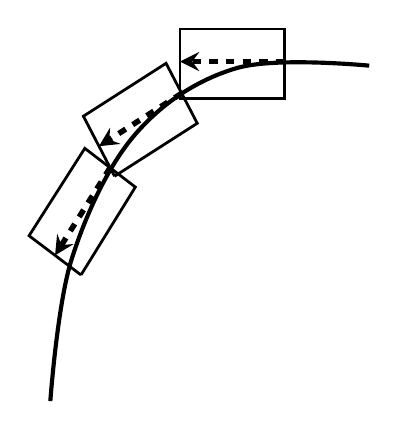
\begin{tikzpicture}[scale=6]
    % Include the PNG file as a background
    % \node[anchor=south west, inner sep=0] (image) at (0,0) {\includegraphics[width=10cm]{curve_rotation.png}};
    
    % Get the dimensions of the image
    % \begin{scope}[x={(image.south east)},y={(image.north west)}]
        % Example TikZ overlay:
        
        \draw[color=black, line width = 1.5] plot[smooth, tension = .6] coordinates{(.15, 0.1) (.195, 0.4) (0.33, 0.665) (0.545, 0.805)  (.825, .81)  }; 

        \draw[black, line width = 1] (.215,.367) -- (.33,.553) -- (.223,.635) -- (.105,.45) -- (.215,.367);
        \draw[black, line width = 1] (.286,.576) -- (.461,.688) -- (.395,.815) -- (.22,.703) -- (.286,.576);
        \draw[black, line width = 1]         (.4245,.74) -- (.645,.74) -- (.645,.8875) -- (.4245,.8875) -- cycle;
 %(.4245,.75) -- (.645,.75) -- (.645,.8975) -- (.4245,.8975) -- (.4245,.75);
        
        \draw[line width=2pt,black,-stealth, dashed] (0.2765, 0.594)--(0.16, 0.4085) node[anchor=south west]{};	
        \draw[line width=2pt,black,-stealth, dashed] (0.428, 0.7515)--(0.253, 0.6395) node[anchor=south west]{};	
        \draw[line width=2pt,black,-stealth, dashed] (0.645, 0.81875)--(0.4245, 0.81875) node[anchor=south west]{};	
        
    % \end{scope}
\end{tikzpicture}
    \caption{A schematic illustration of curve tracking with rotation.}
    \label{fig:curve_rotation}
\end{figure}


\algrenewcommand\algorithmicrequire{\textbf{Input}:}
\algrenewcommand\algorithmicensure{\textbf{Output}:}

\begin{algorithm}[ht]
	\caption{UnitaryTransformation}
 \label{algo:transform}
\begin{algorithmic}[1]
\Require  
\begin{itemize}
    \item A regular curve $C=\{c_1,\dots, c_{n-1}\}\subset\mathbb{Q}[X_1,\dots, X_n]$, and
    \item a point $x=(x_1,\dots,x_n)\in \mathbb{Q}^n$ approximating a point on the curve $C$.
\end{itemize}
\Ensure \begin{itemize}

    \item A transformed curve $\hat{C}$,
    \item a transformed point $\hat{x}$, and
    \item unitary matrices $U$ and $V^\star$.
\end{itemize} 
%\State {Define $C_{x_n}$ by plugging in $X_n=x_n$ for the curve $C$.}
\State {Compute the SVD of $JC(x)=U\Sigma V^\star$\\
Set $\hat{C}=U^\star C(V(X))$.\\
Set $\hat{x}=V^\star x$.\\
Return $(\hat{C},\hat{x}, U, V^\star)$.}

 \end{algorithmic}
 \end{algorithm}

For a regular curve $C$ and point $x$, let $U\Sigma V^\star$ be the SVD of $JC(x)$, and $\hat{x}$ the corresponding image of $x$ under this rotation.  We observe that applying this transformation results in a curve $\hat{C}$ with $\|\hat{C}(\hat{x})\|=\|C(x)\|$. Furthermore, we have that
    $$
    J\hat{C}(\hat{x})= U^\star JC(x)V=U^\star U\Sigma V^\star V=\Sigma.
    $$
We observe that $\Sigma$ is an $(n-1)\times n$ matrix whose last column consists of all zeros. Hence, $\ker J\hat{C}(\hat{x})=\langle e_n\rangle$. When $x$ and $y$ are points on the curve $C$, we know that $V^\star x$ and $V^\star y$ are also points on the curve $\hat{C}$. Moreover, since $V^\star$ is unitary, we have
\[\|\hat{x}-\hat{y}\|=\|V^\star x-V^\star y\|=\|x-y\|.\]

\begin{remark}
We note that \Cref{algo:transform} requires the computation of the singular value decomposition. For rigorous computation, we perform this computation using interval arithmetic so $U$, $\Sigma$, and $V^\star$ are all represented by interval matrices with arbitrary small intervals.  In this case, the diagonal structure and the column of zeros of $\Sigma$ are both maintained.  Since these matrices can be made with arbitrarily small intervals, any subsequent calculation can be made as precise as needed.
\end{remark}

%This unitary transformation will be applied at each step of constructing an interval box that covers the curve. This transformation allows for effective tracking by aligning the curve to track the direction of its kernel vector.

To avoid excessive use of $\hat{C}$ and $\hat{x}$, we always assume that the curve $C$ has been replaced by $\hat{C}$ and $x$ by $\hat{x}$.  Then, we combine this approach with \Cref{def:approximate_solution} to arrive at the following: for a regular curve $C\subset \mathbb{R}^n$, we say that a point $x=(x_1,\dots, x_n)\in \mathbb{R}^n$ is a \emph{$\rho$-approximate solution} to $C$ if $x_{-n}$ is a $\rho$-approximate solution to $C_{x_n}$. In this case, an associated solution $x^\star$ is a point on the curve $C$ where the last coordinate satisfies $X_n=x_n$.

\subsection{Curve prediction}

The core idea of our certified curve tracking algorithm is to construct a series of regions that begin from one point on (or near) the curve and cover a portion of the curve.
The Krawczyk test is applied to these regions to ensure that only one arc of the curve is contained within each region and the curve behaves nicely within the region. To construct such a tube, we use a numerical approximation of the curve (referred to as a \emph{prediction}) and create a region around this approximation with a fixed radius. If the Krawczyk test from \Cref{algo:Krawczyk-test} passes for this region, we proceed to the next step of tracking.

Two methods for curve prediction have been recently proposed in the literature for certified homotopy continuation \cite{duff2024certified,guillemot2024validated}.  In \cite[Algorithm 2]{duff2024certified}, the authors exploit the predictor-corrector method (see, e.g., \cite[Section 2.3]{sommese2005numerical}) for a prediction of the curve.  On the other hand, \cite[Section 6.3]{guillemot2024validated} employs a higher-order approximation of the curve obtained from a point on the curve and a tangent vector. The Taylor model (see \cite[Section 9.3]{moore2009introduction}) is applied to construct a curved interval box bounding this higher-order approximation.  One of the notable differences between these two prediction methods is the use of the step size and a corrector. The predictor algorithm in \cite{duff2024certified} requires the desired step size as input to correct a specific point from a prediction. In contrast, \cite{guillemot2024validated} derives an appropriate step size and does not need a step size as input. 

For a curve $C$, and a point $x$, we denote a prediction of the curve by $X(\eta):[0,\infty)\rightarrow \mathbb{R}^{n-1}$ such that $(X(0),x_n)=x$. The choice of the algorithm to produce such a prediction may be chosen by the user. For a fixed radius $r$, when the algorithm from \cite{duff2024certified} is chosen, we denote this algorithm by $\text{Predictor}(C,x,r,h)$ with a desired step size $h$, or $\text{Predictor}(C,x,r)$ when the prediction algorithm from \cite{guillemot2024validated} is chosen.  Since the choice of prediction is a user-defined choice, in our images we draw enclosing boxes for the prediction tube to illustrate the structure even the true prediction tube may be curved.

\subsection{Refinement}

Since it is difficult to access an exact point on the curve, we must apply the prediction algorithm to a point close to the curve.  The more accurate a given point is, the more precise the prediction will be, and the corresponding tracking will be more efficient.  The refinement step replaces a given prediction by a better prediction, leading to better behavior for the predictor.  \Cref{algo:meta_refine} performs this refinement.  In particular, it takes a $\rho$-approximate solution $x$ with an associated solution $x^\star$ to $C$ as an input and returns a point $x$ and $r$ such that all points in $x+r\tau[-1,0]^n$ are $\tau$-approximate solutions to $C$ for $\tau\in (0,1)$. In this case, a point $y\in x+r\tau[-1,0]^n$ and its associated solution $y^\star$ share the same last coordinate, that is, $y_n=y_n^\star$.  In \Cref{sec:curve_tracking_algorithm}, we illustrate why refining the region $x+r\tau[-1,0]^n$ and replacing $x$ with a better approximate, are both useful in our algorithms.

\begin{algorithm}[ht]
	\caption{RefineSolution}
 \label{algo:meta_refine}
\begin{algorithmic}[1]
\Require  
\begin{itemize}
    \item A regular curve $C=\{c_1,\dots, c_{n-1}\}\subset\mathbb{Q}[X_1,\dots,X_n]$,
    \item a $\rho$-approximate solution $x=(x_1,\dots, x_n)$ to $C$ with a radius $0<r<1$ and an $(n-1)\times (n-1)$ invertible matrix $A$, and
    \item a constant $\tau\in (0,1)$ representing a desired accuracy.
\end{itemize}
\Ensure A $\tau$-approximate solution $x$ with a corresponding radius $r$ and an $(n-1)\times (n-1)$ invertible matrix $A$.
\State{Set $x_{-n}=(x_1,\dots, x_{n-1})$}
\State{Set $I=[-1,0]^{n-1}\in\mathbb{IQ}^{n-1}$}
\While{$\text{KrawczykTest}(C_{x_n+[-r\tau,0]}, x_{-n}+r\tau I, r, A, \tau)=False$}
\State{Set $x_{-n}=x_{-n}-AC_{x_n}(x_{-n})$}
\State{Set $x=(x_{-n},x_n)$}
\State{Set $r=\frac{1}{2}r$}
    \State{Set $A=JC_{x_n}(x_{-n})^{-1}$}
\EndWhile
\While{$2r\leq 1$ and 

$\!\!\!\text{KrawczykTest}(C_{x_n+[-r\tau,0]}, x_{-n}+r\tau I, 2r, A, \tau)=True$}\label{line:while_loop_in_Refine}
\State{Set $r=2r$.}
\EndWhile
\State{Return $x,r,A$.}
 \end{algorithmic}
 \end{algorithm}

As \Cref{algo:meta_refine} may refine a $\rho$-approximate solution to an approximate solution with smaller $\rho$, we can use this algorithm to subdivide the computed regions for a curve. Subdividing these regions is needed when we want a finer curve approximation with a smaller tubular neighborhood. This feature plays an important role in computing the isotopic approximation of a projection of a curve, see \Cref{sec:approximation} for additional details.

We remark that \Cref{algo:meta_refine} is inspired by \cite[Algorithm 2]{guillemot2024validated}. For the completeness, we provide the correctness and termination statement for the algorithm. The detailed analysis can be found in \cite[Section 4.2]{guillemot2024validated} 
\begin{lemma}
\Cref{algo:meta_refine} returns a $\tau$-approximate solution and terminates within finitely many iterations.
\end{lemma}
\begin{proof}
    The input $x$ is a $\rho$-approximate solution, so the map $g(x)=x-AF(x)$ is a $\rho$-Lipschitz continuous function. Also, $x+r\tau[-1,0]^n$ converges to $x$ as $r$ converges to $0$. Therefore, if the first while loop iterates infinitely many times, a point $x$ converges to an exact point on the curve. Furthermore, if $r$ converges to $0$, then $\|K\|$ converges to $0$ where 
    $$K=-\frac{1}{r}A F(x)+\left(I_n-A\square JF(x+rB)\right)B.$$
    %{\color{blue} (Kisun: Check this. Does not $\frac{1}{r}$ prevent $\|K\|\rightarrow0$?)}
    Therefore, the first loop must terminate within finitely many iterations.  The second loop enlarges the radius without changing the result of the Krawczyk test. It must terminate in finitely many iterations since $r$ can only be doubled finitely many times before $r$ is greater than $\frac{1}{2}$.
\end{proof}

The first while loop reduces the radius at each iteration, potentially resulting in a narrow region. Tracking using a narrow interval box can be ineffective because a narrow box results in a narrow curve, strongly controlling the shape of the curve.  The second while loop enlarges the radius to avoid this.

\subsection{Stopping criterion}

We consider two stopping criteria for curve tracking. For a regular curve $C$ in $\mathbb{R}^n$ and a $\rho$-approximate solution $x$ to $C$ with the radius $r$, we suppose that the user provides a compact region of interest $D$ that contains $x$. Tracking terminates whenever we prove that the curve is closed or a newly constructed interval region $I$ intersects with the boundary of $D$. To conclude that the curve $C$ is closed, we check if $I$ intersects with an interval vector $J = x+r\rho[-1,1]^n$. If they intersect, we refine both independently. If the refinement of $J$ is contained in $I$, then we conclude that the curve is closed. If the refinement of $J$ does not intersect $I$ (or its refinement), we continue tracking the curve. We denote these criteria by $\text{StoppingCriterion}(D,x,C)$.
% SHOULD THIS BE: CONTAINS THE DISK AROUND x that contains x^* and passes the Krawczyck test (if not refine both x and the path coming in).

\subsection{Curve tracking algorithm}\label{sec:curve_tracking_algorithm}

We propose \Cref{algo:certified_curve_tracking} to track a regular curve $C$ in $\mathbb{R}^n$ starting with the point $x$.  We recall that the singular value decomposition uses interval arithmetic, so there may be roundoff error in its computation.  Hence, we require that the precision has been increased to make $\|VV^\star- I_n\|$ as small as needed.  Similarly, the computation of any inverses in the algorithm can be made precise enough so that any subsequent error is as small as necessary.  


\begin{algorithm}[ht]
	\caption{CertifiedCurveTracking}
 \label{algo:certified_curve_tracking}
\begin{algorithmic}[1]
\Require  
\begin{itemize}
    \item A regular curve $C=\{c_1,\dots, c_{n-1}\}\subset\mathbb{Q}[X_1,\dots, X_n]$,
    \item an approximate solution $x\in\mathbb{Q}^n$ to the curve $C$,
    \item a constant $h>0$,
    \item a compact region $D$,
    \item constants $\rho\in(0,\frac{1}{2}]$ and $\tau\in(\frac{1}2,1)$
\end{itemize}
\Ensure {\begin{itemize}
    \item A set of interval regions $\mathcal{I}$, and
    \item a $\rho$-approximate solution $x$ of $C$ outside $D$ or a certificate that $C$ is a closed curve.
\end{itemize}}
\State{Set $(\hat{C},\hat{x}, U, V^\star)=\text{UnitaryTransformation}(C,x)$.}
\State{Set $A= J\hat{C}_{\hat{x}_n}(\hat{x}_{-n})^{-1}$.}
\State{Set $\mathcal{I}=\emptyset$.}
\While{$\text{StoppingCriterion}(D,x,C)=False$}
\State{Set $h=\frac{5}{4}h$.}
\State{Set $(\hat{x}, r, A) =\text{RefineSolution}(\hat{C},\hat{x},r,A,\rho)$.}\label{line:6}
\State{Set $x=V\hat{x}$.}\label{line:rotate_back}
\State{Set $(\hat{C},\hat{x}, U, V^\star)=\text{UnitaryTransformation}(C,x)$.}\label{line:unitary_transformation}
\State{Set $A= J\hat{C}_{\hat{x}_n}(\hat{x}_{-n})^{-1}$.}
\State{Set $\hat{X}(\eta)=\left\{\begin{array}{ll}
    \hat{x}_{-n} & \text{ if }\eta<0  \\
    X(\eta)=\text{Predictor}(\hat{C},\hat{x},r,h) & \text{ if } \eta\geq 0
\end{array}\right.$.}\label{line:retract}
%\State{Set $X(\eta)=\text{Predictor}(\hat{C},\hat{x},r,h)$.}
\While{$\text{KrawczykTest}(\hat{C}_{\hat{x}_n+[-r\rho,h]},\hat{X}([-r\rho,h]),r,A,\tau)=False$}\label{line:10}
\State{$h=\frac{h}{2}$.}
\State{Set $X(\eta)=\text{Predictor}(\hat{C},\hat{x},r,h)$.}
\EndWhile
\State{Set $\mathcal{I}=\mathcal{I}\cup\{V\cdot(\hat{X}([-r\rho,h]),\hat{x}_n+[-r\rho,h])^\top\}$.}
\If{$I\cap J\ne\emptyset$ for any non-adjacent $I,J\in \mathcal{I}$ (except if the StoppingCriterion holds).}
\State{Break. Try again with a smaller $\rho$.}
\EndIf
\State{Set $\hat{x}=(X(h),\hat{x}_n+h)$.}\label{line:update}
\EndWhile
\State{Return $x$ or a conclusion that $C$ is a closed curve.}
 \end{algorithmic}
 \end{algorithm}


\begin{lemma}
     %$\text{KrawczykTest}(\hat{C}_{\hat{x}_n+[-r\rho,h]},\hat{X}([-r\rho,h]),r,A,\tau)$ 
     \Cref{line:10} of \Cref{algo:certified_curve_tracking} returns $True$ for some $h>0$.
\end{lemma}
\begin{proof}
%    To avoid abusing notations, we denote $\hat{X}\cup X(\eta)$ by $X(\eta)$ and $\hat{x}_n+[-r\rho,0]$ by $\hat{x}_n$. 
Define 
$$    K(\eta)=-\frac{1}{r}A \hat{C}_{\hat{x}_n+\eta}(\hat{X}(\eta))\\+\left(I_n-A\square J\hat{C}_{\hat{x}_n+\eta}(\hat{X}(\eta)+rB)\right)B$$ from the Krawczyk test in \Cref{line:10}.
    We show that 
    $\|K([-r\rho,h])\|< \tau$
    for some $h>0$ after sufficiently many iterations of the while loop in  \Cref{line:10}.
    When $h$ converges to $0$, the vector $(\hat{X}([-r\rho,h]),\hat{x}_n+[-r\rho,h])$ converges to $(\hat{x}_{-n},\hat{x}_n+[-r\rho,0])$. Hence, there is some sufficiently small $h>0$ such that $\|K([-r\rho,h])\|< \rho$ because $\|K([-r\rho,0])\|<\rho$ from \Cref{line:6}. When the norm is sufficiently small, the Krawczyk test succeeds.  Since the norm is a continuous function of $h$, the result follows.
\end{proof}
% I MADE A CHANGE to line 16, is it OK?
% Good.

The vector $\hat{X}(\eta)$ in \Cref{line:retract} is for constructing an interval extended backwards to cover the curve without any gaps. By evaluating $(\hat{X}(\eta),\hat{x}_n+\eta)$ over the interval $[-r\rho, h]$, the next step of the approximation completely covers the portion of the boundary of the previous interval region that contains the exiting curve.  Without extending the interval backwards, the intervals may not completely cover the curve (see \Cref{fig:retract_box}). Since refinement makes the initial tangent vector closer to the curve's tangent vector, the required backwards component shrinks and the curve will not deviate from the extended part.

\begin{figure}
    \centering
    
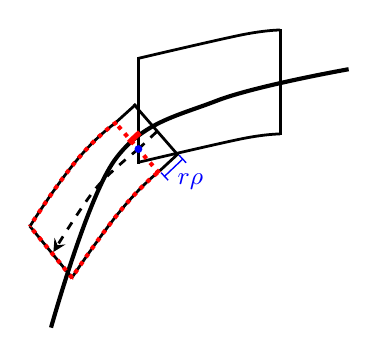
\begin{tikzpicture}[scale=6]
    % Draw smooth curved path
    \draw[color=black, line width = 1.5] plot[smooth, tension = .6] coordinates{
         (.195, 0.31) (0.33, 0.665) (0.545, 0.79) (.825, .857)  
    }; 
    
   
    % Draw the curved pipe (thick tube-like shape)
    \draw[black, line width = 1, rounded corners=0.02cm] 
        (.68,.718) -- (.68,.942);
    \draw[black, line width = 1, rounded corners=0.02cm] 
        (.38,.657) -- (.38,.882);
 
    \draw[color=black, line width = 1] plot[smooth, tension = .6] coordinates{
        (.38, .66) (.60, .71) (.68, .72)  
    }; 
    
    \draw[color=black, line width = 1] plot[smooth, tension = .6] coordinates{
        (.38, .88)  (.60, .93) (.68, .94)  
    }; 


         \draw[dashed, line width = 1] 
        (.38,.688) -- (.419,.725); % Reduced the length but kept the slope

    % Lowered dashed tangent arrow
    \draw[line width=1pt,black,-stealth, dashed] plot[smooth, tension = .6] coordinates{
        (0.38, .688) (0.29, .605)  (0.2, 0.47) % Shifted y-values downward
    }; 

         \draw[color=blue,, line width = .5] 
        (.428,.638) -- (.443,.622); % Reduced the length but kept the slope     
         \draw[color=blue,, line width = .5] 
        (.466,.675) -- (.481,.659); % Reduced the length but kept the slope     
         \draw[color=blue,, line width = .5] 
        (.435,.63) -- (.474,.667); % Reduced the length but kept the slope
        % blue circle node at (.38, .688)
    \node[blue, inner sep=1pt] at (0.49, .62) {{\small$r\rho$}};


     % Draw shorter middle segment with same slope
    \draw[ line width = 1] 
        (.464,.675) -- (.37,.783); % Reduced the length but kept the slope
    \draw[ line width = 1] 
        (.24,.415) -- (.15,.525); % Lowered slightly
    \draw[ line width = 1] 
        (.464,.678) -- (.423,.64); % Reduced the length but kept the slope
    \draw[ line width = 1] 
        (.375,.783) -- (.333,.745); % Reduced the length but kept the slope


    
       % Lowered curved tube around the arrow
    \draw[color=black, line width = 1] plot[smooth, tension = .9] coordinates{
        (0.42, .6375) (0.34, .555) (0.238, .414)  % Shifted downward
    }; 
    
    \draw[color=black, line width = 1] plot[smooth, tension = .9] coordinates{
        (0.334, .745) (0.25, .665) (0.15, .524)  % Shifted downward
    }; 
       
     % Draw shorter middle segment with same slope
    \draw[red, line width = 1.5,dotted] 
        (.424,.637) -- (.33,.745); % Reduced the length but kept the slope
    \draw[red, line width = 1.5,dotted] 
        (.24,.415) -- (.15,.525); % Lowered slightly



 % Lowered curved tube around the arrow
    \draw[color=red, line width = 1.5,dotted] plot[smooth, tension = .9] coordinates{
        (0.42, .6375) (0.34, .555) (0.238, .414)  % Shifted downward
    }; 
    
    \draw[color=red, line width = 1.5,dotted] plot[smooth, tension = .9] coordinates{
        (0.334, .745) (0.25, .665) (0.15, .524)  % Shifted downward
    }; 
    \draw[color=red, line width = 2] plot[smooth, tension = .9] coordinates{
        (0.383, .723) (0.37, .711) (0.36, .701)  % Shifted downward
    }; 
    
        % blue circle node at (.38, .688)
    \node[circle, fill=blue, inner sep=1pt] at (0.38, .688) {};
 

\end{tikzpicture}

    \caption{The blue dot represents refined $\hat{x}$ from \Cref{line:6} in \Cref{algo:certified_curve_tracking}. The dashed arrow describes the prediction $\hat{X}$. The red dashed box constructed from $\hat{x}$ does not cover the curve completely. The solid magenta portion of the curve shows the small uncovered gap when the red dashed box is used. It is covered by the interval extended backward by $r\rho$. The solid black boxes represent actual intervals computed to cover the curve.}
    \label{fig:retract_box}
\end{figure}



\begin{lemma}
    In \Cref{algo:certified_curve_tracking}, $\hat{x}=(X(h),\hat{x}_n+h)$ from \Cref{line:update} is a $\tau$-approximate solution to $\hat{C}$.
\end{lemma}
\begin{proof}
For a point $\hat{x}$ obtained from \Cref{line:unitary_transformation}, define
$$K(\eta)=-\frac{1}{r}A \hat{C}_{\hat{x}_n+\eta}(X(\eta))\\+\left(I_n-A\square J\hat{C}_{\hat{x}_n+\eta}(X(\eta)+rB)\right)B.$$ 
    Due to the second while loop, we have $\|K(h)\|< \tau$
    for any $h\in [-r\rho,h]$. This implies that $(X(h),\hat{x}_n+h)$ in \Cref{line:update} is a $\tau$-approximate solution to $\hat{C}$.
\end{proof}


\begin{thm}
\Cref{algo:certified_curve_tracking} terminates.
\end{thm}
\begin{proof}
    We prove that the a sequence of points $x$ obtained in \Cref{line:rotate_back} does not converge to a point until it satisfies the stopping criterion.  Suppose that the sequence does converge before satisfying the stopping criterion.  This means that $h$ must be halved infinitely many times as we repeat the second while loop in \Cref{line:10}.  Define $$K(\eta,\lambda)=-\frac{1}{\lambda}A\hat{C}_{\hat{x}_n+\eta}(\hat{X}(\eta))+\left(I_n-A\square J\hat{C}_{\hat{x}_n+\eta}(\hat{X}(\eta)+\lambda B)\right)B.$$
    Then, we have $\|K([-r\rho,h],r)\|>\tau$ for infinitely many $h$.
    On the other hand, $\|K([-r\rho,0],r)\|< \rho$ because of \Cref{line:6} in the algorithm. 
    
    If there is $r_0>0$ such that $r\geq r_0$ at each iteration, then we have $\lim\limits_{h\rightarrow 0}\|K([-r_0\rho,h],r_0)\|<\rho$ which contradicts the fact that $\|K([-r\rho,h],r)\|>\tau>\rho$ for infinitely many $h$.
    Therefore, we may assume that $r$ becomes arbitrarily small due to refinement in  \Cref{line:6}. %In this case, the matrix $A$ converges to $J\hat{C}_{\hat{x}_n}(\hat{x})^{-1}$. 
    Then, whenever $r<1$ is returned from \Cref{line:6}, we have
    $\|K([-r\rho,0],2r)\|>\rho$ because of the second loop in \Cref{line:while_loop_in_Refine} of \Cref{algo:meta_refine}.
    Furthermore,
    since $\square J\hat{C}_{\hat{x}_n+[-r\rho,0]}(\hat{X}([-r\rho,0])+2rB)$ converges to $J\hat{C}_{\hat{x}_n}(\hat{x}_{-n})$ as $r$ converges to $0$, for any $0<\epsilon<1$, there is $r_0>0$ such that 
    \[\left\|I_n-A\square J\hat{C}_{\hat{x}_n+[-r\rho,0]}(\hat{X}([-r\rho,0])+2rB)\right\|<\epsilon\]
    whenever $r<r_0$.
    Therefore, we have $$\left\|-\frac{1}{2r}A\hat{C}_{\hat{x}_n+[-r\rho,0]}(\hat{X}([-r\rho,0])\right\|+\epsilon \geq \|K([-r\rho,0],2r)\|>\rho.$$ This contradicts the inequality $\|K([-r\rho,0],r)\|<\rho$.
\end{proof}

For a detailed analysis of the homotopy path tracking algorithm with adaptive precision, see \cite[Section 5.3]{guillemot2024validated}.

We say that the collection of all interval regions computed from \Cref{algo:certified_curve_tracking} is a \emph{tubular neighborhood} of the curve $C$ and denote this by $\mathcal{A}(C)$ (see \Cref{fig:tubular_nbd}).  We observe that by reducing $\rho$ as needed, we can make the Hausdorff distance between the approximation and the curve as small as desired.  In addition, if we wish to create an approximation to the curve itself, we may construct a path within the interval regions connecting, connecting them sequentially.

\begin{figure}[h]
    \centering
    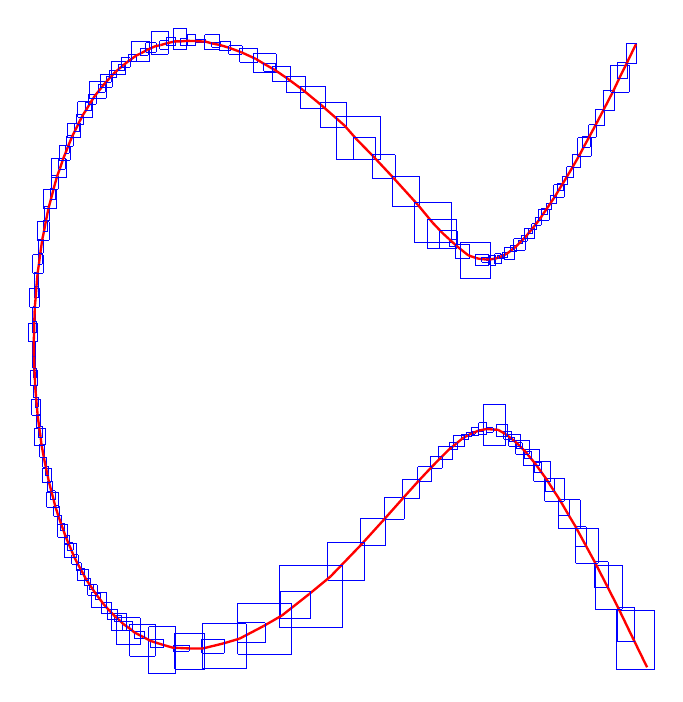
\begin{tikzpicture}[scale=2]
\draw[color=blue,line width=.1mm] (1.7672680232739488,-2.0664276180518364) --(2.0087726377482005,-2.0664276180518364);
\draw[color=blue,line width=.1mm] (1.7672680232739488,-2.0664276180518364) --(1.7672680232739488,-1.6893021508780812);
\draw[color=blue,line width=.1mm] (1.7672680232739488,-1.6893021508780812) --(2.0087726377482005,-1.6893021508780812);
\draw[color=blue,line width=.1mm] (2.0087726377482005,-2.0664276180518364) --(2.0087726377482005,-1.6893021508780812);
\draw[color=red,line width=.3mm] (1.8781805340635234,-1.8824363931215293) --(1.9599484516112473,-2.049832969311939);
\draw[color=blue,line width=.1mm] (1.7716136339414867,-1.8854079322162776) --(1.8801321565235036,-1.8854079322162776);
\draw[color=blue,line width=.1mm] (1.7716136339414867,-1.8854079322162776) --(1.7716136339414867,-1.6714068221598624);
\draw[color=blue,line width=.1mm] (1.7716136339414867,-1.6714068221598624) --(1.8801321565235036,-1.6714068221598624);
\draw[color=blue,line width=.1mm] (1.8801321565235036,-1.8854079322162776) --(1.8801321565235036,-1.6714068221598624);
\draw[color=red,line width=.3mm] (1.7767254282171432,-1.67286902239068) --(1.8781805340635234,-1.8824363931215293);
\draw[color=blue,line width=.1mm] (1.6302064135322565,-1.6815560621802874) --(1.8009900240810806,-1.6815560621802874);
\draw[color=blue,line width=.1mm] (1.6302064135322565,-1.6815560621802874) --(1.6302064135322565,-1.3999609182250865);
\draw[color=blue,line width=.1mm] (1.6302064135322565,-1.3999609182250865) --(1.8009900240810806,-1.3999609182250865);
\draw[color=blue,line width=.1mm] (1.8009900240810806,-1.6815560621802874) --(1.8009900240810806,-1.3999609182250865);
\draw[color=red,line width=.3mm] (1.7107078883063518,-1.543175201736721) --(1.7767254282171432,-1.67286902239068);
\draw[color=blue,line width=.1mm] (1.6246794914188534,-1.545047619461742) --(1.714516507607393,-1.545047619461742);
\draw[color=blue,line width=.1mm] (1.6246794914188534,-1.545047619461742) --(1.6246794914188534,-1.3790463484709232);
\draw[color=blue,line width=.1mm] (1.6246794914188534,-1.3790463484709232) --(1.714516507607393,-1.3790463484709232);
\draw[color=blue,line width=.1mm] (1.714516507607393,-1.545047619461742) --(1.714516507607393,-1.3790463484709232);
\draw[color=red,line width=.3mm] (1.6275671315150533,-1.3813863103053532) --(1.7107078883063518,-1.543175201736721);
\draw[color=blue,line width=.1mm] (1.505826286765492,-1.3897086218721901) --(1.649645110386169,-1.3897086218721901);
\draw[color=blue,line width=.1mm] (1.505826286765492,-1.3897086218721901) --(1.505826286765492,-1.1685735184956079);
\draw[color=blue,line width=.1mm] (1.505826286765492,-1.1685735184956079) --(1.649645110386169,-1.1685735184956079);
\draw[color=blue,line width=.1mm] (1.649645110386169,-1.3897086218721901) --(1.649645110386169,-1.1685735184956079);
\draw[color=red,line width=.3mm] (1.5732974782965872,-1.2814780189874624) --(1.6275671315150533,-1.3813863103053532);
\draw[color=blue,line width=.1mm] (1.5045542742210811,-1.2820175978193893) --(1.5739186904012596,-1.2820175978193893);
\draw[color=blue,line width=.1mm] (1.5045542742210811,-1.2820175978193893) --(1.5045542742210811,-1.1562211032795622);
\draw[color=blue,line width=.1mm] (1.5045542742210811,-1.1562211032795622) --(1.5739186904012596,-1.1562211032795622);
\draw[color=blue,line width=.1mm] (1.5739186904012596,-1.2820175978193893) --(1.5739186904012596,-1.1562211032795622);
\draw[color=red,line width=.3mm] (1.5055491936117682,-1.1565580081968663) --(1.5732974782965872,-1.2814780189874624);
\draw[color=blue,line width=.1mm] (1.3965613869350981,-1.1688026037902286) --(1.5356914635614138,-1.1688026037902286);
\draw[color=blue,line width=.1mm] (1.3965613869350981,-1.1688026037902286) --(1.3965613869350981,-0.9848402449299296);
\draw[color=blue,line width=.1mm] (1.3965613869350981,-0.9848402449299296) --(1.5356914635614138,-0.9848402449299296);
\draw[color=blue,line width=.1mm] (1.5356914635614138,-1.1688026037902286) --(1.5356914635614138,-0.9848402449299296);
\draw[color=red,line width=.3mm] (1.4600595186483567,-1.0802441898741932) --(1.5055491936117682,-1.1565580081968663);
\draw[color=blue,line width=.1mm] (1.397861757259802,-1.083847039233679) --(1.46385547932236,-1.083847039233679);
\draw[color=blue,line width=.1mm] (1.397861757259802,-1.083847039233679) --(1.397861757259802,-0.9821813212183956);
\draw[color=blue,line width=.1mm] (1.397861757259802,-0.9821813212183956) --(1.46385547932236,-0.9821813212183956);
\draw[color=blue,line width=.1mm] (1.46385547932236,-1.083847039233679) --(1.46385547932236,-0.9821813212183956);
\draw[color=red,line width=.3mm] (1.4040241069241337,-0.984400649262553) --(1.4600595186483567,-1.0802441898741932);
\draw[color=blue,line width=.1mm] (1.3108957419780056,-0.9970413204954904) --(1.4326597775242265,-0.9970413204954904);
\draw[color=blue,line width=.1mm] (1.3108957419780056,-0.9970413204954904) --(1.3108957419780056,-0.848520230801959);
\draw[color=blue,line width=.1mm] (1.3108957419780056,-0.848520230801959) --(1.4326597775242265,-0.848520230801959);
\draw[color=blue,line width=.1mm] (1.4326597775242265,-0.9970413204954904) --(1.4326597775242265,-0.848520230801959);
\draw[color=red,line width=.3mm] (1.3660078964111328,-0.9263153869790889) --(1.4040241069241337,-0.984400649262553);
\draw[color=blue,line width=.1mm] (1.3133776777964115,-0.9300944935203429) --(1.3696486327522464,-0.9300944935203429);
\draw[color=blue,line width=.1mm] (1.3133776777964115,-0.9300944935203429) --(1.3133776777964115,-0.8509090689149584);
\draw[color=blue,line width=.1mm] (1.3133776777964115,-0.8509090689149584) --(1.3696486327522464,-0.8509090689149584);
\draw[color=blue,line width=.1mm] (1.3696486327522464,-0.9300944935203429) --(1.3696486327522464,-0.8509090689149584);
\draw[color=red,line width=.3mm] (1.319289052841324,-0.8532365699336388) --(1.3660078964111328,-0.9263153869790889);
\draw[color=blue,line width=.1mm] (1.238776983803436,-0.8665996714392499) --(1.3467539417262373,-0.8665996714392499);
\draw[color=blue,line width=.1mm] (1.238776983803436,-0.8665996714392499) --(1.238776983803436,-0.744858684031275);
\draw[color=blue,line width=.1mm] (1.238776983803436,-0.744858684031275) --(1.3467539417262373,-0.744858684031275);
\draw[color=blue,line width=.1mm] (1.3467539417262373,-0.8665996714392499) --(1.3467539417262373,-0.744858684031275);
\draw[color=red,line width=.3mm] (1.2872302973110021,-0.8094751011557337) --(1.319289052841324,-0.8532365699336388);
\draw[color=blue,line width=.1mm] (1.2425151488696586,-0.813309863269718) --(1.2905430553783093,-0.813309863269718);
\draw[color=blue,line width=.1mm] (1.2425151488696586,-0.813309863269718) --(1.2425151488696586,-0.7519369311066508);
\draw[color=blue,line width=.1mm] (1.2425151488696586,-0.7519369311066508) --(1.2905430553783093,-0.7519369311066508);
\draw[color=blue,line width=.1mm] (1.2905430553783093,-0.813309863269718) --(1.2905430553783093,-0.7519369311066508);
\draw[color=red,line width=.3mm] (1.2478941317485206,-0.7542986488708995) --(1.2872302973110021,-0.8094751011557337);
\draw[color=blue,line width=.1mm] (1.1774347435416876,-0.7688273801642735) --(1.2743625293219685,-0.7688273801642735);
\draw[color=blue,line width=.1mm] (1.1774347435416876,-0.7688273801642735) --(1.1774347435416876,-0.6667758535069679);
\draw[color=blue,line width=.1mm] (1.1774347435416876,-0.6667758535069679) --(1.2743625293219685,-0.6667758535069679);
\draw[color=blue,line width=.1mm] (1.2743625293219685,-0.7688273801642735) --(1.2743625293219685,-0.6667758535069679);
\draw[color=red,line width=.3mm] (1.2205626552006665,-0.7218842704355275) --(1.2478941317485206,-0.7542986488708995);
\draw[color=blue,line width=.1mm] (1.1821178677757798,-0.7259439140366841) --(1.2236263484494356,-0.7259439140366841);
\draw[color=blue,line width=.1mm] (1.1821178677757798,-0.7259439140366841) --(1.1821178677757798,-0.678367550139733);
\draw[color=blue,line width=.1mm] (1.1821178677757798,-0.678367550139733) --(1.2236263484494356,-0.678367550139733);
\draw[color=blue,line width=.1mm] (1.2236263484494356,-0.7259439140366841) --(1.2236263484494356,-0.678367550139733);
\draw[color=red,line width=.3mm] (1.1870929081886685,-0.6808675303943873) --(1.2205626552006665,-0.7218842704355275);
\draw[color=blue,line width=.1mm] (1.1251003540712037,-0.6968762738725593) --(1.2121727942614444,-0.6968762738725593);
\draw[color=blue,line width=.1mm] (1.1251003540712037,-0.6968762738725593) --(1.1251003540712037,-0.6091135409988886);
\draw[color=blue,line width=.1mm] (1.1251003540712037,-0.6091135409988886) --(1.2121727942614444,-0.6091135409988886);
\draw[color=blue,line width=.1mm] (1.2121727942614444,-0.6968762738725593) --(1.2121727942614444,-0.6091135409988886);
\draw[color=red,line width=.3mm] (1.1635775016099554,-0.657504764435173) --(1.1870929081886685,-0.6808675303943873);
\draw[color=blue,line width=.1mm] (1.130230530818156,-0.6619629786624212) --(1.166419851781032,-0.6619629786624212);
\draw[color=blue,line width=.1mm] (1.130230530818156,-0.6619629786624212) --(1.130230530818156,-0.6250086943660501);
\draw[color=blue,line width=.1mm] (1.130230530818156,-0.6250086943660501) --(1.166419851781032,-0.6250086943660501);
\draw[color=blue,line width=.1mm] (1.166419851781032,-0.6619629786624212) --(1.166419851781032,-0.6250086943660501);
\draw[color=red,line width=.3mm] (1.1348471656731136,-0.627753508807633) --(1.1635775016099554,-0.657504764435173);
\draw[color=blue,line width=.1mm] (1.0807228844458998,-0.6452398105758455) --(1.1575263517987744,-0.6452398105758455);
\draw[color=blue,line width=.1mm] (1.0807228844458998,-0.6452398105758455) --(1.0807228844458998,-0.5681408207166221);
\draw[color=blue,line width=.1mm] (1.0807228844458998,-0.5681408207166221) --(1.1575263517987744,-0.5681408207166221);
\draw[color=blue,line width=.1mm] (1.1575263517987744,-0.6452398105758455) --(1.1575263517987744,-0.5681408207166221);
\draw[color=red,line width=.3mm] (1.1145450112177422,-0.6116314975650117) --(1.1348471656731136,-0.627753508807633);
\draw[color=blue,line width=.1mm] (1.0856186440554325,-0.6166073898683467) --(1.1171150828353007,-0.6166073898683467);
\draw[color=blue,line width=.1mm] (1.0856186440554325,-0.6166073898683467) --(1.0856186440554325,-0.5877973090581295);
\draw[color=blue,line width=.1mm] (1.0856186440554325,-0.5877973090581295) --(1.1171150828353007,-0.5877973090581295);
\draw[color=blue,line width=.1mm] (1.1171150828353007,-0.6166073898683467) --(1.1171150828353007,-0.5877973090581295);
\draw[color=red,line width=.3mm] (1.0897946954312563,-0.5908596275637578) --(1.1145450112177422,-0.6116314975650117);
\draw[color=blue,line width=.1mm] (1.0504006617870887,-0.6001382805002538) --(1.1008367249328417,-0.6001382805002538);
\draw[color=blue,line width=.1mm] (1.0504006617870887,-0.6001382805002538) --(1.0504006617870887,-0.5519191966918913);
\draw[color=blue,line width=.1mm] (1.0504006617870887,-0.5519191966918913) --(1.1008367249328417,-0.5519191966918913);
\draw[color=blue,line width=.1mm] (1.1008367249328417,-0.6001382805002538) --(1.1008367249328417,-0.5519191966918913);
\draw[color=red,line width=.3mm] (1.0571764528350176,-0.5670399641124714) --(1.0897946954312563,-0.5908596275637578);
\draw[color=blue,line width=.1mm] (1.0019251441700816,-0.5870104145354336) --(1.075911606603904,-0.5870104145354336);
\draw[color=blue,line width=.1mm] (1.0019251441700816,-0.5870104145354336) --(1.0019251441700816,-0.5093068376512011);
\draw[color=blue,line width=.1mm] (1.0019251441700816,-0.5093068376512011) --(1.075911606603904,-0.5093068376512011);
\draw[color=blue,line width=.1mm] (1.075911606603904,-0.5870104145354336) --(1.075911606603904,-0.5093068376512011);
\draw[color=red,line width=.3mm] (1.0134217160342744,-0.5418512748788171) --(1.0571764528350176,-0.5670399641124714);
\draw[color=blue,line width=.1mm] (0.9188963914990697,-0.641356953530104) --(1.0616289914820616,-0.641356953530104);
\draw[color=blue,line width=.1mm] (0.9188963914990697,-0.641356953530104) --(0.9188963914990697,-0.38382281932839857);
\draw[color=blue,line width=.1mm] (0.9188963914990697,-0.38382281932839857) --(1.0616289914820616,-0.38382281932839857);
\draw[color=blue,line width=.1mm] (1.0616289914820616,-0.641356953530104) --(1.0616289914820616,-0.38382281932839857);
\draw[color=red,line width=.3mm] (0.9804871990659366,-0.5403897813304323) --(1.0134217160342744,-0.5418512748788171);
\draw[color=blue,line width=.1mm] (0.9389903401020417,-0.5557365766568986) --(0.9812793316664609,-0.5557365766568986);
\draw[color=blue,line width=.1mm] (0.9389903401020417,-0.5557365766568986) --(0.9389903401020417,-0.5291164902870954);
\draw[color=blue,line width=.1mm] (0.9389903401020417,-0.5291164902870954) --(0.9812793316664609,-0.5291164902870954);
\draw[color=blue,line width=.1mm] (0.9812793316664609,-0.5557365766568986) --(0.9812793316664609,-0.5291164902870954);
\draw[color=red,line width=.3mm] (0.9411048168596245,-0.5366988594421276) --(0.9804871990659366,-0.5403897813304323);
\draw[color=blue,line width=.1mm] (0.8902498483181801,-0.5738928871532994) --(0.9425146618265529,-0.5738928871532994);
\draw[color=blue,line width=.1mm] (0.8902498483181801,-0.5738928871532994) --(0.8902498483181801,-0.4969606662007141);
\draw[color=blue,line width=.1mm] (0.8902498483181801,-0.4969606662007141) --(0.9425146618265529,-0.4969606662007141);
\draw[color=blue,line width=.1mm] (0.9425146618265529,-0.5738928871532994) --(0.9425146618265529,-0.4969606662007141);
\draw[color=red,line width=.3mm] (0.9166397076205808,-0.5418587068012264) --(0.9411048168596245,-0.5366988594421276);
\draw[color=blue,line width=.1mm] (0.8861939019132188,-0.5495745360905718) --(0.9170840594467955,-0.5495745360905718);
\draw[color=blue,line width=.1mm] (0.8861939019132188,-0.5495745360905718) --(0.8861939019132188,-0.5415910821840814);
\draw[color=blue,line width=.1mm] (0.8861939019132188,-0.5415910821840814) --(0.9170840594467955,-0.5415910821840814);
\draw[color=blue,line width=.1mm] (0.9170840594467955,-0.5495745360905718) --(0.9170840594467955,-0.5415910821840814);
\draw[color=red,line width=.3mm] (0.8864831864538545,-0.5483697384839672) --(0.9166397076205808,-0.5418587068012264);
\draw[color=blue,line width=.1mm] (0.8436052880043805,-0.5770719299186035) --(0.8918604909469083,-0.5770719299186035);
\draw[color=blue,line width=.1mm] (0.8436052880043805,-0.5770719299186035) --(0.8436052880043805,-0.5288015436241417);
\draw[color=blue,line width=.1mm] (0.8436052880043805,-0.5288015436241417) --(0.8918604909469083,-0.5288015436241417);
\draw[color=blue,line width=.1mm] (0.8918604909469083,-0.5770719299186035) --(0.8918604909469083,-0.5288015436241417);
\draw[color=red,line width=.3mm] (0.8687298106754318,-0.5561295713618026) --(0.8864831864538545,-0.5483697384839672);
\draw[color=blue,line width=.1mm] (0.8453771146029567,-0.5682794164591856) --(0.8700486988251896,-0.5682794164591856);
\draw[color=blue,line width=.1mm] (0.8453771146029567,-0.5682794164591856) --(0.8453771146029567,-0.5537347729829294);
\draw[color=blue,line width=.1mm] (0.8453771146029567,-0.5537347729829294) --(0.8700486988251896,-0.5537347729829294);
\draw[color=blue,line width=.1mm] (0.8700486988251896,-0.5682794164591856) --(0.8700486988251896,-0.5537347729829294);
\draw[color=red,line width=.3mm] (0.8463157033970179,-0.564914288543173) --(0.8687298106754318,-0.5561295713618026);
\draw[color=blue,line width=.1mm] (0.8152964493756426,-0.5838791943421131) --(0.8491306156765913,-0.5838791943421131);
\draw[color=blue,line width=.1mm] (0.8152964493756426,-0.5838791943421131) --(0.8152964493756426,-0.5567692762448462);
\draw[color=blue,line width=.1mm] (0.8152964493756426,-0.5567692762448462) --(0.8491306156765913,-0.5567692762448462);
\draw[color=blue,line width=.1mm] (0.8491306156765913,-0.5838791943421131) --(0.8491306156765913,-0.5567692762448462);
\draw[color=red,line width=.3mm] (0.8192704430633434,-0.5781098105626478) --(0.8463157033970179,-0.564914288543173);
\draw[color=blue,line width=.1mm] (0.7810404486647654,-0.6043329123359602) --(0.8234385669041272,-0.6043329123359602);
\draw[color=blue,line width=.1mm] (0.7810404486647654,-0.6043329123359602) --(0.7810404486647654,-0.5681975280468781);
\draw[color=blue,line width=.1mm] (0.7810404486647654,-0.5681975280468781) --(0.8234385669041272,-0.5681975280468781);
\draw[color=blue,line width=.1mm] (0.8234385669041272,-0.6043329123359602) --(0.8234385669041272,-0.5681975280468781);
\draw[color=red,line width=.3mm] (0.7869248586079061,-0.597311712090956) --(0.8192704430633434,-0.5781098105626478);
\draw[color=blue,line width=.1mm] (0.7324256817108279,-0.6459232169423843) --(0.8020956009157261,-0.6459232169423843);
\draw[color=blue,line width=.1mm] (0.7324256817108279,-0.6459232169423843) --(0.7324256817108279,-0.5745182181696067);
\draw[color=blue,line width=.1mm] (0.7324256817108279,-0.5745182181696067) --(0.8020956009157261,-0.5745182181696067);
\draw[color=blue,line width=.1mm] (0.8020956009157261,-0.6459232169423843) --(0.8020956009157261,-0.5745182181696067);
\draw[color=red,line width=.3mm] (0.7507922974268535,-0.6276626707246948) --(0.7869248586079061,-0.597311712090956);
\draw[color=blue,line width=.1mm] (0.7025323753116706,-0.6687097975421791) --(0.7541896077093722,-0.6687097975421791);
\draw[color=blue,line width=.1mm] (0.7025323753116706,-0.6687097975421791) --(0.7025323753116706,-0.6246169960844424);
\draw[color=blue,line width=.1mm] (0.7025323753116706,-0.6246169960844424) --(0.7541896077093722,-0.6246169960844424);
\draw[color=blue,line width=.1mm] (0.7541896077093722,-0.6687097975421791) --(0.7541896077093722,-0.6246169960844424);
\draw[color=red,line width=.3mm] (0.7049802515704019,-0.6644828265701573) --(0.7507922974268535,-0.6276626707246948);
\draw[color=blue,line width=.1mm] (0.6322448945430375,-0.731868778263873) --(0.7213068869023851,-0.731868778263873);
\draw[color=blue,line width=.1mm] (0.6322448945430375,-0.731868778263873) --(0.6322448945430375,-0.6442675092506246);
\draw[color=blue,line width=.1mm] (0.6322448945430375,-0.6442675092506246) --(0.7213068869023851,-0.6442675092506246);
\draw[color=blue,line width=.1mm] (0.7213068869023851,-0.731868778263873) --(0.7213068869023851,-0.6442675092506246);
\draw[color=red,line width=.3mm] (0.652654011765161,-0.7161410042956926) --(0.7049802515704019,-0.6644828265701573);
\draw[color=blue,line width=.1mm] (0.5835848780220831,-0.7852936328406922) --(0.6570690225448916,-0.7852936328406922);
\draw[color=blue,line width=.1mm] (0.5835848780220831,-0.7852936328406922) --(0.5835848780220831,-0.7122121048876561);
\draw[color=blue,line width=.1mm] (0.5835848780220831,-0.7122121048876561) --(0.6570690225448916,-0.7122121048876561);
\draw[color=blue,line width=.1mm] (0.6570690225448916,-0.7852936328406922) --(0.6570690225448916,-0.7122121048876561);
\draw[color=red,line width=.3mm] (0.5885258275647198,-0.7818944273207767) --(0.652654011765161,-0.7161410042956926);
\draw[color=blue,line width=.1mm] (0.5045450164940863,-0.8689785580362606) --(0.592248914577505,-0.8689785580362606);
\draw[color=blue,line width=.1mm] (0.5045450164940863,-0.8689785580362606) --(0.5045450164940863,-0.7769143358317616);
\draw[color=blue,line width=.1mm] (0.5045450164940863,-0.7769143358317616) --(0.592248914577505,-0.7769143358317616);
\draw[color=blue,line width=.1mm] (0.592248914577505,-0.8689785580362606) --(0.592248914577505,-0.7769143358317616);
\draw[color=red,line width=.3mm] (0.5098344095880745,-0.8654731815939952) --(0.5885258275647198,-0.7818944273207767);
\draw[color=blue,line width=.1mm] (0.40509368403443347,-0.9775868041362902) --(0.515971675222751,-0.9775868041362902);
\draw[color=blue,line width=.1mm] (0.40509368403443347,-0.9775868041362902) --(0.40509368403443347,-0.8576627888871645);
\draw[color=blue,line width=.1mm] (0.40509368403443347,-0.8576627888871645) --(0.515971675222751,-0.8576627888871645);
\draw[color=blue,line width=.1mm] (0.515971675222751,-0.9775868041362902) --(0.515971675222751,-0.8576627888871645);
\draw[color=red,line width=.3mm] (0.41375805859188786,-0.9720544423161769) --(0.5098344095880745,-0.8654731815939952);
\draw[color=blue,line width=.1mm] (0.29115137355279097,-1.1082496592934143) --(0.41618102849338123,-1.1082496592934143);
\draw[color=blue,line width=.1mm] (0.29115137355279097,-1.1082496592934143) --(0.29115137355279097,-0.9690128656729025);
\draw[color=blue,line width=.1mm] (0.29115137355279097,-0.9690128656729025) --(0.41618102849338123,-0.9690128656729025);
\draw[color=blue,line width=.1mm] (0.41618102849338123,-1.1082496592934143) --(0.41618102849338123,-0.9690128656729025);
\draw[color=red,line width=.3mm] (0.29457203653306385,-1.1060952088014842) --(0.41375805859188786,-0.9720544423161769);
\draw[color=blue,line width=.1mm] (0.1396734157694991,-1.2776839594146496) --(0.3006325119292851,-1.2776839594146496);
\draw[color=blue,line width=.1mm] (0.1396734157694991,-1.2776839594146496) --(0.1396734157694991,-1.1022026630373931);
\draw[color=blue,line width=.1mm] (0.1396734157694991,-1.1022026630373931) --(0.3006325119292851,-1.1022026630373931);
\draw[color=blue,line width=.1mm] (0.3006325119292851,-1.2776839594146496) --(0.3006325119292851,-1.1022026630373931);
\draw[color=red,line width=.3mm] (0.1439662529075623,-1.2721886012745063) --(0.29457203653306385,-1.1060952088014842);
\draw[color=blue,line width=.1mm] (-0.06712085839228984,-1.4963970370520618) --(0.167286657338419,-1.4963970370520618);
\draw[color=blue,line width=.1mm] (-0.06712085839228984,-1.4963970370520618) --(-0.06712085839228984,-1.2562551472731647);
\draw[color=blue,line width=.1mm] (-0.06712085839228984,-1.2562551472731647) --(0.167286657338419,-1.2562551472731647);
\draw[color=blue,line width=.1mm] (0.167286657338419,-1.4963970370520618) --(0.167286657338419,-1.2562551472731647);
\draw[color=red,line width=.3mm] (-0.050602238036016975,-1.4739027499520392) --(0.1439662529075623,-1.2721886012745063);
\draw[color=blue,line width=.1mm] (-0.37443356391332994,-1.7952620038949467) --(0.027127348461077117,-1.7952620038949467);
\draw[color=blue,line width=.1mm] (-0.37443356391332994,-1.7952620038949467) --(-0.37443356391332994,-1.40256099227821);
\draw[color=blue,line width=.1mm] (-0.37443356391332994,-1.40256099227821) --(0.027127348461077117,-1.40256099227821);
\draw[color=blue,line width=.1mm] (0.027127348461077117,-1.7952620038949467) --(0.027127348461077117,-1.40256099227821);
\draw[color=red,line width=.3mm] (-0.18600175713432093,-1.5853910248772636) --(-0.050602238036016975,-1.4739027499520392);
\draw[color=blue,line width=.1mm] (-0.36787641738771987,-1.7376586232645186) --(-0.17490182622566414,-1.7376586232645186);
\draw[color=blue,line width=.1mm] (-0.36787641738771987,-1.7376586232645186) --(-0.36787641738771987,-1.5701672203218313);
\draw[color=blue,line width=.1mm] (-0.36787641738771987,-1.5701672203218313) --(-0.17490182622566414,-1.5701672203218313);
\draw[color=blue,line width=.1mm] (-0.17490182622566414,-1.7376586232645186) --(-0.17490182622566414,-1.5701672203218313);
\draw[color=red,line width=.3mm] (-0.3581467615247824,-1.7207612855769907) --(-0.18600175713432093,-1.5853910248772636);
\draw[color=blue,line width=.1mm] (-0.6385276070118917,-1.9660741852344235) --(-0.2958892308429851,-1.9660741852344235);
\draw[color=blue,line width=.1mm] (-0.6385276070118917,-1.9660741852344235) --(-0.6385276070118917,-1.6415416922168096);
\draw[color=blue,line width=.1mm] (-0.6385276070118917,-1.6415416922168096) --(-0.2958892308429851,-1.6415416922168096);
\draw[color=blue,line width=.1mm] (-0.2958892308429851,-1.9660741852344235) --(-0.2958892308429851,-1.6415416922168096);
\draw[color=red,line width=.3mm] (-0.47706853164217233,-1.7891509295770525) --(-0.3581467615247824,-1.7207612855769907);
\draw[color=blue,line width=.1mm] (-0.6392086931097909,-1.8949476278689414) --(-0.46478232560340604,-1.8949476278689414);
\draw[color=blue,line width=.1mm] (-0.6392086931097909,-1.8949476278689414) --(-0.6392086931097909,-1.7658601140905827);
\draw[color=blue,line width=.1mm] (-0.6392086931097909,-1.7658601140905827) --(-0.46478232560340604,-1.7658601140905827);
\draw[color=blue,line width=.1mm] (-0.46478232560340604,-1.8949476278689414) --(-0.46478232560340604,-1.7658601140905827);
\draw[color=red,line width=.3mm] (-0.6286556235856421,-1.868582435119811) --(-0.47706853164217233,-1.7891509295770525);
\draw[color=blue,line width=.1mm] (-0.8650617366556177,-2.05815875934435) --(-0.5843755169671128,-2.05815875934435);
\draw[color=blue,line width=.1mm] (-0.8650617366556177,-2.05815875934435) --(-0.8650617366556177,-1.7742217796295692);
\draw[color=blue,line width=.1mm] (-0.8650617366556177,-1.7742217796295692) --(-0.5843755169671128,-1.7742217796295692);
\draw[color=blue,line width=.1mm] (-0.5843755169671128,-2.05815875934435) --(-0.5843755169671128,-1.7742217796295692);
\draw[color=red,line width=.3mm] (-0.731715287741503,-1.8989239697714217) --(-0.6286556235856421,-1.868582435119811);
\draw[color=blue,line width=.1mm] (-0.8675029841760248,-1.9589704341334186) --(-0.7250734465705305,-1.9589704341334186);
\draw[color=blue,line width=.1mm] (-0.8675029841760248,-1.9589704341334186) --(-0.8675029841760248,-1.8733366456427507);
\draw[color=blue,line width=.1mm] (-0.8675029841760248,-1.8733366456427507) --(-0.7250734465705305,-1.8733366456427507);
\draw[color=blue,line width=.1mm] (-0.7250734465705305,-1.9589704341334186) --(-0.7250734465705305,-1.8733366456427507);
\draw[color=red,line width=.3mm] (-0.8616776461442567,-1.9305480244930389) --(-0.731715287741503,-1.8989239697714217);
\draw[color=blue,line width=.1mm] (-1.0392674941301672,-2.061770149823319) --(-0.8481016771599975,-2.061770149823319);
\draw[color=blue,line width=.1mm] (-1.0392674941301672,-2.061770149823319) --(-1.0392674941301672,-1.8343000727147272);
\draw[color=blue,line width=.1mm] (-1.0392674941301672,-1.8343000727147272) --(-0.8481016771599975,-1.8343000727147272);
\draw[color=blue,line width=.1mm] (-0.8481016771599975,-2.061770149823319) --(-0.8481016771599975,-1.8343000727147272);
\draw[color=red,line width=.3mm] (-0.9458406212286052,-1.930418083551855) --(-0.8616776461442567,-1.9305480244930389);
\draw[color=blue,line width=.1mm] (-1.0503268840051145,-1.9467895575256575) --(-0.9457739386501611,-1.9467895575256575);
\draw[color=blue,line width=.1mm] (-1.0503268840051145,-1.9467895575256575) --(-1.0503268840051145,-1.9107502090667863);
\draw[color=blue,line width=.1mm] (-1.0503268840051145,-1.9107502090667863) --(-0.9457739386501611,-1.9107502090667863);
\draw[color=blue,line width=.1mm] (-0.9457739386501611,-1.9467895575256575) --(-0.9457739386501611,-1.9107502090667863);
\draw[color=red,line width=.3mm] (-1.0502650713697776,-1.9259579418014068) --(-0.9458406212286052,-1.930418083551855);
\draw[color=blue,line width=.1mm] (-1.2050622009044796,-2.0896854509519507) --(-1.0323209626438379,-2.0896854509519507);
\draw[color=blue,line width=.1mm] (-1.2050622009044796,-2.0896854509519507) --(-1.2050622009044796,-1.7921076018283235);
\draw[color=blue,line width=.1mm] (-1.2050622009044796,-1.7921076018283235) --(-1.0323209626438379,-1.7921076018283235);
\draw[color=blue,line width=.1mm] (-1.0323209626438379,-2.0896854509519507) --(-1.0323209626438379,-1.7921076018283235);
\draw[color=red,line width=.3mm] (-1.1134313272348175,-1.9076347888191836) --(-1.0502650713697776,-1.9259579418014068);
\draw[color=blue,line width=.1mm] (-1.1958478672772688,-1.9211617095990967) --(-1.1098383209778038,-1.9211617095990967);
\draw[color=blue,line width=.1mm] (-1.1958478672772688,-1.9211617095990967) --(-1.1958478672772688,-1.8731336200855602);
\draw[color=blue,line width=.1mm] (-1.1958478672772688,-1.8731336200855602) --(-1.1098383209778038,-1.8731336200855602);
\draw[color=blue,line width=.1mm] (-1.1098383209778038,-1.9211617095990967) --(-1.1098383209778038,-1.8731336200855602);
\draw[color=red,line width=.3mm] (-1.19137435772902,-1.8833644291105496) --(-1.1134313272348175,-1.9076347888191836);
\draw[color=blue,line width=.1mm] (-1.325562337516305,-1.9799974007295589) --(-1.1636741919074776,-1.9799974007295589);
\draw[color=blue,line width=.1mm] (-1.325562337516305,-1.9799974007295589) --(-1.325562337516305,-1.777427179342709);
\draw[color=blue,line width=.1mm] (-1.325562337516305,-1.777427179342709) --(-1.1636741919074776,-1.777427179342709);
\draw[color=blue,line width=.1mm] (-1.1636741919074776,-1.9799974007295589) --(-1.1636741919074776,-1.777427179342709);
\draw[color=red,line width=.3mm] (-1.236479559787688,-1.8590370900320776) --(-1.19137435772902,-1.8833644291105496);
\draw[color=blue,line width=.1mm] (-1.2962484666059462,-1.864835971688631) --(-1.2316765566502434,-1.864835971688631);
\draw[color=blue,line width=.1mm] (-1.2962484666059462,-1.864835971688631) --(-1.2962484666059462,-1.8207364934629415);
\draw[color=blue,line width=.1mm] (-1.2962484666059462,-1.8207364934629415) --(-1.2316765566502434,-1.8207364934629415);
\draw[color=blue,line width=.1mm] (-1.2316765566502434,-1.864835971688631) --(-1.2316765566502434,-1.8207364934629415);
\draw[color=red,line width=.3mm] (-1.2933059666086344,-1.830201930460379) --(-1.236479559787688,-1.8590370900320776);
\draw[color=blue,line width=.1mm] (-1.4086461935734567,-1.9060713969522933) --(-1.2597354538815286,-1.9060713969522933);
\draw[color=blue,line width=.1mm] (-1.4086461935734567,-1.9060713969522933) --(-1.4086461935734567,-1.7345732382384906);
\draw[color=blue,line width=.1mm] (-1.4086461935734567,-1.7345732382384906) --(-1.2597354538815286,-1.7345732382384906);
\draw[color=blue,line width=.1mm] (-1.2597354538815286,-1.9060713969522933) --(-1.2597354538815286,-1.7345732382384906);
\draw[color=red,line width=.3mm] (-1.324367428704593,-1.8048094534651153) --(-1.2933059666086344,-1.830201930460379);
\draw[color=blue,line width=.1mm] (-1.373146254443639,-1.8163356813882499) --(-1.3110265513440418,-1.8163356813882499);
\draw[color=blue,line width=.1mm] (-1.373146254443639,-1.8163356813882499) --(-1.373146254443639,-1.7571985071106835);
\draw[color=blue,line width=.1mm] (-1.373146254443639,-1.7571985071106835) --(-1.3110265513440418,-1.7571985071106835);
\draw[color=blue,line width=.1mm] (-1.3110265513440418,-1.8163356813882499) --(-1.3110265513440418,-1.7571985071106835);
\draw[color=red,line width=.3mm] (-1.3649657687106003,-1.775995678733918) --(-1.324367428704593,-1.8048094534651153);
\draw[color=blue,line width=.1mm] (-1.4437148318085433,-1.8134579900100818) --(-1.3436736036948473,-1.8134579900100818);
\draw[color=blue,line width=.1mm] (-1.4437148318085433,-1.8134579900100818) --(-1.4437148318085433,-1.710551072206161);
\draw[color=blue,line width=.1mm] (-1.4437148318085433,-1.710551072206161) --(-1.3436736036948473,-1.710551072206161);
\draw[color=blue,line width=.1mm] (-1.3436736036948473,-1.8134579900100818) --(-1.3436736036948473,-1.710551072206161);
\draw[color=red,line width=.3mm] (-1.3874682401556748,-1.7543508107627355) --(-1.3649657687106003,-1.775995678733918);
\draw[color=blue,line width=.1mm] (-1.4216641645549297,-1.759994438882797) --(-1.379402405095423,-1.759994438882797);
\draw[color=blue,line width=.1mm] (-1.4216641645549297,-1.759994438882797) --(-1.4216641645549297,-1.7195121705051242);
\draw[color=blue,line width=.1mm] (-1.4216641645549297,-1.7195121705051242) --(-1.379402405095423,-1.7195121705051242);
\draw[color=blue,line width=.1mm] (-1.379402405095423,-1.759994438882797) --(-1.379402405095423,-1.7195121705051242);
\draw[color=red,line width=.3mm] (-1.4167178020657212,-1.7287150087505423) --(-1.3874682401556748,-1.7543508107627355);
\draw[color=blue,line width=.1mm] (-1.4699704656098702,-1.74765238252901) --(-1.4039921748638817,-1.74765238252901);
\draw[color=blue,line width=.1mm] (-1.4699704656098702,-1.74765238252901) --(-1.4699704656098702,-1.6817873704104171);
\draw[color=blue,line width=.1mm] (-1.4699704656098702,-1.6817873704104171) --(-1.4039921748638817,-1.6817873704104171);
\draw[color=blue,line width=.1mm] (-1.4039921748638817,-1.74765238252901) --(-1.4039921748638817,-1.6817873704104171);
\draw[color=red,line width=.3mm] (-1.4507967723723816,-1.694012326786943) --(-1.4167178020657212,-1.7287150087505423);
\draw[color=blue,line width=.1mm] (-1.5066687343473388,-1.707426931273454) --(-1.4405689670069917,-1.707426931273454);
\draw[color=blue,line width=.1mm] (-1.5066687343473388,-1.707426931273454) --(-1.5066687343473388,-1.64008692294106);
\draw[color=blue,line width=.1mm] (-1.5066687343473388,-1.64008692294106) --(-1.4405689670069917,-1.64008692294106);
\draw[color=blue,line width=.1mm] (-1.4405689670069917,-1.707426931273454) --(-1.4405689670069917,-1.64008692294106);
\draw[color=red,line width=.3mm] (-1.4914475679198036,-1.6488209519334018) --(-1.4507967723723816,-1.694012326786943);
\draw[color=blue,line width=.1mm] (-1.5669776621127418,-1.6712425253705048) --(-1.4726774702632717,-1.6712425253705048);
\draw[color=blue,line width=.1mm] (-1.5669776621127418,-1.6712425253705048) --(-1.5669776621127418,-1.574788096512381);
\draw[color=blue,line width=.1mm] (-1.5669776621127418,-1.574788096512381) --(-1.4726774702632717,-1.574788096512381);
\draw[color=blue,line width=.1mm] (-1.4726774702632717,-1.6712425253705048) --(-1.4726774702632717,-1.574788096512381);
\draw[color=red,line width=.3mm] (-1.514318802769595,-1.6184432502057662) --(-1.4914475679198036,-1.6488209519334018);
\draw[color=blue,line width=.1mm] (-1.543791510777279,-1.6187542411609206) --(-1.5132891230764438,-1.6187542411609206);
\draw[color=blue,line width=.1mm] (-1.543791510777279,-1.6187542411609206) --(-1.543791510777279,-1.580108970298304);
\draw[color=blue,line width=.1mm] (-1.543791510777279,-1.580108970298304) --(-1.5132891230764438,-1.580108970298304);
\draw[color=blue,line width=.1mm] (-1.5132891230764438,-1.6187542411609206) --(-1.5132891230764438,-1.580108970298304);
\draw[color=red,line width=.3mm] (-1.5429001145429513,-1.5805270576864092) --(-1.514318802769595,-1.6184432502057662);
\draw[color=blue,line width=.1mm] (-1.5924910461406219,-1.591329930536932) --(-1.532356721546221,-1.591329930536932);
\draw[color=blue,line width=.1mm] (-1.5924910461406219,-1.591329930536932) --(-1.5924910461406219,-1.5246712452038365);
\draw[color=blue,line width=.1mm] (-1.5924910461406219,-1.5246712452038365) --(-1.532356721546221,-1.5246712452038365);
\draw[color=blue,line width=.1mm] (-1.532356721546221,-1.591329930536932) --(-1.532356721546221,-1.5246712452038365);
\draw[color=red,line width=.3mm] (-1.5593330232802813,-1.5558008561362517) --(-1.5429001145429513,-1.5805270576864092);
\draw[color=blue,line width=.1mm] (-1.5812292681460998,-1.556543842007597) --(-1.557543058743587,-1.556543842007597);
\draw[color=blue,line width=.1mm] (-1.5812292681460998,-1.556543842007597) --(-1.5812292681460998,-1.5238768056646967);
\draw[color=blue,line width=.1mm] (-1.5812292681460998,-1.5238768056646967) --(-1.557543058743587,-1.5238768056646967);
\draw[color=blue,line width=.1mm] (-1.557543058743587,-1.556543842007597) --(-1.557543058743587,-1.5238768056646967);
\draw[color=red,line width=.3mm] (-1.5801321832664612,-1.525089034785198) --(-1.5593330232802813,-1.5558008561362517);
\draw[color=blue,line width=.1mm] (-1.6126431162012778,-1.5299336704215079) --(-1.5754631861820854,-1.5299336704215079);
\draw[color=blue,line width=.1mm] (-1.6126431162012778,-1.5299336704215079) --(-1.6126431162012778,-1.4830060771223201);
\draw[color=blue,line width=.1mm] (-1.6126431162012778,-1.4830060771223201) --(-1.5754631861820854,-1.4830060771223201);
\draw[color=blue,line width=.1mm] (-1.5754631861820854,-1.5299336704215079) --(-1.5754631861820854,-1.4830060771223201);
\draw[color=red,line width=.3mm] (-1.6050343804031995,-1.4859789218707038) --(-1.5801321832664612,-1.525089034785198);
\draw[color=blue,line width=.1mm] (-1.6565723653880513,-1.4990107925898994) --(-1.5893173436166352,-1.4990107925898994);
\draw[color=blue,line width=.1mm] (-1.6565723653880513,-1.4990107925898994) --(-1.6565723653880513,-1.4267961910284723);
\draw[color=blue,line width=.1mm] (-1.6565723653880513,-1.4267961910284723) --(-1.5893173436166352,-1.4267961910284723);
\draw[color=blue,line width=.1mm] (-1.5893173436166352,-1.4990107925898994) --(-1.5893173436166352,-1.4267961910284723);
\draw[color=red,line width=.3mm] (-1.6184041636422968,-1.4602197901382195) --(-1.6050343804031995,-1.4859789218707038);
\draw[color=blue,line width=.1mm] (-1.6410550363693992,-1.4629394189089253) --(-1.6105736328504654,-1.4629394189089253);
\draw[color=blue,line width=.1mm] (-1.6410550363693992,-1.4629394189089253) --(-1.6410550363693992,-1.4242654365936942);
\draw[color=blue,line width=.1mm] (-1.6410550363693992,-1.4242654365936942) --(-1.6105736328504654,-1.4242654365936942);
\draw[color=blue,line width=.1mm] (-1.6105736328504654,-1.4629394189089253) --(-1.6105736328504654,-1.4242654365936942);
\draw[color=red,line width=.3mm] (-1.6362519863037668,-1.4286993141979054) --(-1.6184041636422968,-1.4602197901382195);
\draw[color=blue,line width=.1mm] (-1.6640217686656524,-1.4321197468216111) --(-1.6323353945629333,-1.4321197468216111);
\draw[color=blue,line width=.1mm] (-1.6640217686656524,-1.4321197468216111) --(-1.6640217686656524,-1.3866915002708835);
\draw[color=blue,line width=.1mm] (-1.6640217686656524,-1.3866915002708835) --(-1.6323353945629333,-1.3866915002708835);
\draw[color=blue,line width=.1mm] (-1.6323353945629333,-1.4321197468216111) --(-1.6323353945629333,-1.3866915002708835);
\draw[color=red,line width=.3mm] (-1.6576391749102348,-1.388790402248582) --(-1.6362519863037668,-1.4286993141979054);
\draw[color=blue,line width=.1mm] (-1.6925422341290604,-1.393574803810397) --(-1.651779944119763,-1.393574803810397);
\draw[color=blue,line width=.1mm] (-1.6925422341290604,-1.393574803810397) --(-1.6925422341290604,-1.335253402857406);
\draw[color=blue,line width=.1mm] (-1.6925422341290604,-1.335253402857406) --(-1.651779944119763,-1.335253402857406);
\draw[color=blue,line width=.1mm] (-1.651779944119763,-1.393574803810397) --(-1.651779944119763,-1.335253402857406);
\draw[color=red,line width=.3mm] (-1.6829938582442148,-1.3381892858051025) --(-1.6576391749102348,-1.388790402248582);
\draw[color=blue,line width=.1mm] (-1.7419001967538386,-1.3516939931399583) --(-1.6619468076279624,-1.3516939931399583);
\draw[color=blue,line width=.1mm] (-1.7419001967538386,-1.3516939931399583) --(-1.7419001967538386,-1.264239794513157);
\draw[color=blue,line width=.1mm] (-1.7419001967538386,-1.264239794513157) --(-1.6619468076279624,-1.264239794513157);
\draw[color=blue,line width=.1mm] (-1.6619468076279624,-1.3516939931399583) --(-1.6619468076279624,-1.264239794513157);
\draw[color=red,line width=.3mm] (-1.695873388717062,-1.3051738520930234) --(-1.6829938582442148,-1.3381892858051025);
\draw[color=blue,line width=.1mm] (-1.7209438466834237,-1.3083667032117647) --(-1.6840524232847949,-1.3083667032117647);
\draw[color=blue,line width=.1mm] (-1.7209438466834237,-1.3083667032117647) --(-1.7209438466834237,-1.2595010449806852);
\draw[color=blue,line width=.1mm] (-1.7209438466834237,-1.2595010449806852) --(-1.6840524232847949,-1.2595010449806852);
\draw[color=blue,line width=.1mm] (-1.6840524232847949,-1.3083667032117647) --(-1.6840524232847949,-1.2595010449806852);
\draw[color=red,line width=.3mm] (-1.7136930535530157,-1.264706348861739) --(-1.695873388717062,-1.3051738520930234);
\draw[color=blue,line width=.1mm] (-1.7426660776149676,-1.2679486959938981) --(-1.7088867792521798,-1.2679486959938981);
\draw[color=blue,line width=.1mm] (-1.7426660776149676,-1.2679486959938981) --(-1.7426660776149676,-1.211648024280937);
\draw[color=blue,line width=.1mm] (-1.7426660776149676,-1.211648024280937) --(-1.7088867792521798,-1.211648024280937);
\draw[color=blue,line width=.1mm] (-1.7088867792521798,-1.2679486959938981) --(-1.7088867792521798,-1.211648024280937);
\draw[color=red,line width=.3mm] (-1.734833630802926,-1.2136376465379068) --(-1.7136930535530157,-1.264706348861739);
\draw[color=blue,line width=.1mm] (-1.7819918429124344,-1.2222354551103023) --(-1.718858663702308,-1.2222354551103023);
\draw[color=blue,line width=.1mm] (-1.7819918429124344,-1.2222354551103023) --(-1.7819918429124344,-1.1430030401587543);
\draw[color=blue,line width=.1mm] (-1.7819918429124344,-1.1430030401587543) --(-1.718858663702308,-1.1430030401587543);
\draw[color=blue,line width=.1mm] (-1.718858663702308,-1.2222354551103023) --(-1.718858663702308,-1.1430030401587543);
\draw[color=red,line width=.3mm] (-1.7458119458812105,-1.180849952695871) --(-1.734833630802926,-1.2136376465379068);
\draw[color=blue,line width=.1mm] (-1.7654571573086009,-1.1826038423084284) --(-1.7380108567023576,-1.1826038423084284);
\draw[color=blue,line width=.1mm] (-1.7654571573086009,-1.1826038423084284) --(-1.7654571573086009,-1.1374473046950626);
\draw[color=blue,line width=.1mm] (-1.7654571573086009,-1.1374473046950626) --(-1.7380108567023576,-1.1374473046950626);
\draw[color=blue,line width=.1mm] (-1.7380108567023576,-1.1826038423084284) --(-1.7380108567023576,-1.1374473046950626);
\draw[color=red,line width=.3mm] (-1.7606719081983206,-1.1403065598588855) --(-1.7458119458812105,-1.180849952695871);
\draw[color=blue,line width=.1mm] (-1.7848267560432054,-1.1425616701268104) --(-1.75666726022175,-1.1425616701268104);
\draw[color=blue,line width=.1mm] (-1.7848267560432054,-1.1425616701268104) --(-1.7848267560432054,-1.0879066529701908);
\draw[color=blue,line width=.1mm] (-1.7848267560432054,-1.0879066529701908) --(-1.75666726022175,-1.0879066529701908);
\draw[color=blue,line width=.1mm] (-1.75666726022175,-1.1425616701268104) --(-1.75666726022175,-1.0879066529701908);
\draw[color=red,line width=.3mm] (-1.77830066320391,-1.0892904707783024) --(-1.7606719081983206,-1.1403065598588855);
\draw[color=blue,line width=.1mm] (-1.808684366967263,-1.0924242232495114) --(-1.7723098789949103,-1.0924242232495114);
\draw[color=blue,line width=.1mm] (-1.808684366967263,-1.0924242232495114) --(-1.808684366967263,-1.0231258596095383);
\draw[color=blue,line width=.1mm] (-1.808684366967263,-1.0231258596095383) --(-1.7723098789949103,-1.0231258596095383);
\draw[color=blue,line width=.1mm] (-1.7723098789949103,-1.0924242232495114) --(-1.7723098789949103,-1.0231258596095383);
\draw[color=red,line width=.3mm] (-1.7989216077917776,-1.0250488443726025) --(-1.77830066320391,-1.0892904707783024);
\draw[color=blue,line width=.1mm] (-1.8524871515373387,-1.0337915134924276) --(-1.7774035333686196,-1.0337915134924276);
\draw[color=blue,line width=.1mm] (-1.8524871515373387,-1.0337915134924276) --(-1.8524871515373387,-0.9378088889253139);
\draw[color=blue,line width=.1mm] (-1.8524871515373387,-0.9378088889253139) --(-1.7774035333686196,-0.9378088889253139);
\draw[color=blue,line width=.1mm] (-1.7774035333686196,-1.0337915134924276) --(-1.7774035333686196,-0.9378088889253139);
\draw[color=red,line width=.3mm] (-1.8087679955603857,-0.9839931921120424) --(-1.7989216077917776,-1.0250488443726025);
\draw[color=blue,line width=.1mm] (-1.830153541487803,-0.9860215930760223) --(-1.7968133928018373,-0.9860215930760223);
\draw[color=blue,line width=.1mm] (-1.830153541487803,-0.9860215930760223) --(-1.830153541487803,-0.9298831659046318);
\draw[color=blue,line width=.1mm] (-1.830153541487803,-0.9298831659046318) --(-1.7968133928018373,-0.9298831659046318);
\draw[color=blue,line width=.1mm] (-1.7968133928018373,-0.9860215930760223) --(-1.7968133928018373,-0.9298831659046318);
\draw[color=red,line width=.3mm] (-1.8228201987785562,-0.9331898061857916) --(-1.8087679955603857,-0.9839931921120424);
\draw[color=blue,line width=.1mm] (-1.8473206128903146,-0.9352730007338653) --(-1.817842175244721,-0.9352730007338653);
\draw[color=blue,line width=.1mm] (-1.8473206128903146,-0.9352730007338653) --(-1.8473206128903146,-0.868093329943655);
\draw[color=blue,line width=.1mm] (-1.8473206128903146,-0.868093329943655) --(-1.817842175244721,-0.868093329943655);
\draw[color=blue,line width=.1mm] (-1.817842175244721,-0.9352730007338653) --(-1.817842175244721,-0.868093329943655);
\draw[color=red,line width=.3mm] (-1.8392082784434285,-0.8693716541639268) --(-1.8228201987785562,-0.9331898061857916);
\draw[color=blue,line width=.1mm] (-1.8812645571924285,-0.8748186370820434) --(-1.822567577535613,-0.8748186370820434);
\draw[color=blue,line width=.1mm] (-1.8812645571924285,-0.8748186370820434) --(-1.8812645571924285,-0.7852824925674753);
\draw[color=blue,line width=.1mm] (-1.8812645571924285,-0.7852824925674753) --(-1.822567577535613,-0.7852824925674753);
\draw[color=blue,line width=.1mm] (-1.822567577535613,-0.8748186370820434) --(-1.822567577535613,-0.7852824925674753);
\draw[color=red,line width=.3mm] (-1.8471172285629804,-0.8289302801566354) --(-1.8392082784434285,-0.8693716541639268);
\draw[color=blue,line width=.1mm] (-1.8631139336077258,-0.8300162927563931) --(-1.8390706369402114,-0.8300162927563931);
\draw[color=blue,line width=.1mm] (-1.8631139336077258,-0.8300162927563931) --(-1.8631139336077258,-0.7768867081696796);
\draw[color=blue,line width=.1mm] (-1.8631139336077258,-0.7768867081696796) --(-1.8390706369402114,-0.7768867081696796);
\draw[color=blue,line width=.1mm] (-1.8390706369402114,-0.8300162927563931) --(-1.8390706369402114,-0.7768867081696796);
\draw[color=red,line width=.3mm] (-1.8581776476700163,-0.7786570065128223) --(-1.8471172285629804,-0.8289302801566354);
\draw[color=blue,line width=.1mm] (-1.8779115946635276,-0.78006257117133) --(-1.8539360674875927,-0.78006257117133);
\draw[color=blue,line width=.1mm] (-1.8779115946635276,-0.78006257117133) --(-1.8779115946635276,-0.7147404466556699);
\draw[color=blue,line width=.1mm] (-1.8779115946635276,-0.7147404466556699) --(-1.8539360674875927,-0.7147404466556699);
\draw[color=blue,line width=.1mm] (-1.8539360674875927,-0.78006257117133) --(-1.8539360674875927,-0.7147404466556699);
\draw[color=red,line width=.3mm] (-1.8709993900879627,-0.7156029525273181) --(-1.8581776476700163,-0.7786570065128223);
\draw[color=blue,line width=.1mm] (-1.8959450701501916,-0.7175168896770532) --(-1.8645970641070742,-0.7175168896770532);
\draw[color=blue,line width=.1mm] (-1.8959450701501916,-0.7175168896770532) --(-1.8959450701501916,-0.6353179751873443);
\draw[color=blue,line width=.1mm] (-1.8959450701501916,-0.6353179751873443) --(-1.8645970641070742,-0.6353179751873443);
\draw[color=blue,line width=.1mm] (-1.8645970641070742,-0.7175168896770532) --(-1.8645970641070742,-0.6353179751873443);
\draw[color=red,line width=.3mm] (-1.8855116502689504,-0.636492436895306) --(-1.8709993900879627,-0.7156029525273181);
\draw[color=blue,line width=.1mm] (-1.9335311950235865,-0.6416309954134742) --(-1.862345747747948,-0.6416309954134742);
\draw[color=blue,line width=.1mm] (-1.9335311950235865,-0.6416309954134742) --(-1.9335311950235865,-0.5335117913551624);
\draw[color=blue,line width=.1mm] (-1.9335311950235865,-0.5335117913551624) --(-1.862345747747948,-0.5335117913551624);
\draw[color=blue,line width=.1mm] (-1.862345747747948,-0.6416309954134742) --(-1.862345747747948,-0.5335117913551624);
\draw[color=red,line width=.3mm] (-1.8912992160169961,-0.5865103537265793) --(-1.8855116502689504,-0.636492436895306);
\draw[color=blue,line width=.1mm] (-1.908148364892931,-0.58764489254023) --(-1.8786381362602145,-0.58764489254023);
\draw[color=blue,line width=.1mm] (-1.908148364892931,-0.58764489254023) --(-1.908148364892931,-0.5224843997558863);
\draw[color=blue,line width=.1mm] (-1.908148364892931,-0.5224843997558863) --(-1.8786381362602145,-0.5224843997558863);
\draw[color=blue,line width=.1mm] (-1.8786381362602145,-0.58764489254023) --(-1.8786381362602145,-0.5224843997558863);
\draw[color=red,line width=.3mm] (-1.9003807959383026,-0.5243336891882053) --(-1.8912992160169961,-0.5865103537265793);
\draw[color=blue,line width=.1mm] (-1.919433604647912,-0.5254952395648904) --(-1.8948519623794535,-0.5254952395648904);
\draw[color=blue,line width=.1mm] (-1.919433604647912,-0.5254952395648904) --(-1.919433604647912,-0.44572011151697705);
\draw[color=blue,line width=.1mm] (-1.919433604647912,-0.44572011151697705) --(-1.8948519623794535,-0.44572011151697705);
\draw[color=blue,line width=.1mm] (-1.8948519623794535,-0.5254952395648904) --(-1.8948519623794535,-0.44572011151697705);
\draw[color=red,line width=.3mm] (-1.9104236538423756,-0.4464328813632412) --(-1.9003807959383026,-0.5243336891882053);
\draw[color=blue,line width=.1mm] (-1.9472088691469456,-0.44927086103486064) --(-1.8917050785308878,-0.44927086103486064);
\draw[color=blue,line width=.1mm] (-1.9472088691469456,-0.44927086103486064) --(-1.9472088691469456,-0.3467950751517171);
\draw[color=blue,line width=.1mm] (-1.9472088691469456,-0.3467950751517171) --(-1.8917050785308878,-0.3467950751517171);
\draw[color=blue,line width=.1mm] (-1.8917050785308878,-0.44927086103486064) --(-1.8917050785308878,-0.3467950751517171);
\draw[color=red,line width=.3mm] (-1.9140686672831073,-0.39744975271109134) --(-1.9104236538423756,-0.4464328813632412);
\draw[color=blue,line width=.1mm] (-1.9253962155083306,-0.39797430057172883) --(-1.9051513034094703,-0.39797430057172883);
\draw[color=blue,line width=.1mm] (-1.9253962155083306,-0.39797430057172883) --(-1.9253962155083306,-0.3355112293162498);
\draw[color=blue,line width=.1mm] (-1.9253962155083306,-0.3355112293162498) --(-1.9051513034094703,-0.3355112293162498);
\draw[color=blue,line width=.1mm] (-1.9051513034094703,-0.39797430057172883) --(-1.9051513034094703,-0.3355112293162498);
\draw[color=red,line width=.3mm] (-1.919925070064486,-0.3363661842520899) --(-1.9140686672831073,-0.39744975271109134);
\draw[color=blue,line width=.1mm] (-1.9341050347029627,-0.3370121840075971) --(-1.914999908261972,-0.3370121840075971);
\draw[color=blue,line width=.1mm] (-1.9341050347029627,-0.3370121840075971) --(-1.9341050347029627,-0.25951243742978286);
\draw[color=blue,line width=.1mm] (-1.9341050347029627,-0.25951243742978286) --(-1.914999908261972,-0.25951243742978286);
\draw[color=blue,line width=.1mm] (-1.914999908261972,-0.3370121840075971) --(-1.914999908261972,-0.25951243742978286);
\draw[color=red,line width=.3mm] (-1.9260788452580886,-0.2599088466609342) --(-1.919925070064486,-0.3363661842520899);
\draw[color=blue,line width=.1mm] (-1.9555377473766733,-0.26136157562855455) --(-1.9092522083260868,-0.26136157562855455);
\draw[color=blue,line width=.1mm] (-1.9555377473766733,-0.26136157562855455) --(-1.9555377473766733,-0.16317224881045342);
\draw[color=blue,line width=.1mm] (-1.9555377473766733,-0.16317224881045342) --(-1.9092522083260868,-0.16317224881045342);
\draw[color=blue,line width=.1mm] (-1.9092522083260868,-0.26136157562855455) --(-1.9092522083260868,-0.16317224881045342);
\draw[color=red,line width=.3mm] (-1.9275560990497573,-0.21196850984526863) --(-1.9260788452580886,-0.2599088466609342);
\draw[color=blue,line width=.1mm] (-1.9354353790034107,-0.21221320912830552) --(-1.9196104174982789,-0.21221320912830552);
\draw[color=blue,line width=.1mm] (-1.9354353790034107,-0.21221320912830552) --(-1.9354353790034107,-0.15171958668746074);
\draw[color=blue,line width=.1mm] (-1.9354353790034107,-0.15171958668746074) --(-1.9196104174982789,-0.15171958668746074);
\draw[color=blue,line width=.1mm] (-1.9196104174982789,-0.21221320912830552) --(-1.9196104174982789,-0.15171958668746074);
\draw[color=red,line width=.3mm] (-1.930560056727541,-0.1521183914186067) --(-1.9275560990497573,-0.21196850984526863);
\draw[color=blue,line width=.1mm] (-1.940600905556812,-0.1523822490369034) --(-1.926046441225799,-0.1523822490369034);
\draw[color=blue,line width=.1mm] (-1.940600905556812,-0.1523822490369034) --(-1.940600905556812,-0.07709780535763772);
\draw[color=blue,line width=.1mm] (-1.940600905556812,-0.07709780535763772) --(-1.926046441225799,-0.07709780535763772);
\draw[color=blue,line width=.1mm] (-1.926046441225799,-0.1523822490369034) --(-1.926046441225799,-0.07709780535763772);
\draw[color=red,line width=.3mm] (-1.9332453840894892,-0.07725971823760056) --(-1.930560056727541,-0.1521183914186067);
\draw[color=blue,line width=.1mm] (-1.946340278423928,-0.0774665752050735) --(-1.9262526936871711,-0.0774665752050735);
\draw[color=blue,line width=.1mm] (-1.946340278423928,-0.0774665752050735) --(-1.946340278423928,0.01648532121001855);
\draw[color=blue,line width=.1mm] (-1.946340278423928,0.01648532121001855) --(-1.9262526936871711,0.01648532121001855);
\draw[color=blue,line width=.1mm] (-1.9262526936871711,-0.0774665752050735) --(-1.9262526936871711,0.01648532121001855);
\draw[color=red,line width=.3mm] (-1.9349447831202837,0.016358385988920497) --(-1.9332453840894892,-0.07725971823760056);
\draw[color=blue,line width=.1mm] (-1.970758891246115,0.01625933629074784) --(-1.9086655072642686,0.01625933629074784);
\draw[color=blue,line width=.1mm] (-1.970758891246115,0.01625933629074784) --(-1.970758891246115,0.13353676712685913);
\draw[color=blue,line width=.1mm] (-1.970758891246115,0.13353676712685913) --(-1.9086655072642686,0.13353676712685913);
\draw[color=blue,line width=.1mm] (-1.9086655072642686,0.01625933629074784) --(-1.9086655072642686,0.13353676712685913);
\draw[color=red,line width=.3mm] (-1.9323327277700482,0.07486975453047989) --(-1.9349447831202837,0.016358385988920497);
\draw[color=blue,line width=.1mm] (-1.9406714659555884,0.07463041365759307) --(-1.917455560949079,0.07463041365759307);
\draw[color=blue,line width=.1mm] (-1.9406714659555884,0.07463041365759307) --(-1.9406714659555884,0.14815647351702535);
\draw[color=blue,line width=.1mm] (-1.9406714659555884,0.14815647351702535) --(-1.917455560949079,0.14815647351702535);
\draw[color=blue,line width=.1mm] (-1.917455560949079,0.07463041365759307) --(-1.917455560949079,0.14815647351702535);
\draw[color=red,line width=.3mm] (-1.9310445280691904,0.14800960403133862) --(-1.9323327277700482,0.07486975453047989);
\draw[color=blue,line width=.1mm] (-1.9418845189375145,0.14777758839832725) --(-1.921205265376558,0.14777758839832725);
\draw[color=blue,line width=.1mm] (-1.9418845189375145,0.14777758839832725) --(-1.9418845189375145,0.2397711222880903);
\draw[color=blue,line width=.1mm] (-1.9418845189375145,0.2397711222880903) --(-1.921205265376558,0.2397711222880903);
\draw[color=blue,line width=.1mm] (-1.921205265376558,0.14777758839832725) --(-1.921205265376558,0.2397711222880903);
\draw[color=red,line width=.3mm] (-1.927857078047677,0.23939302316628908) --(-1.9310445280691904,0.14800960403133862);
\draw[color=blue,line width=.1mm] (-1.9602693508132765,0.23807961990016424) --(-1.898211378975346,0.23807961990016424);
\draw[color=blue,line width=.1mm] (-1.9602693508132765,0.23807961990016424) --(-1.9602693508132765,0.3553452585626664);
\draw[color=blue,line width=.1mm] (-1.9602693508132765,0.3553452585626664) --(-1.898211378975346,0.3553452585626664);
\draw[color=blue,line width=.1mm] (-1.898211378975346,0.23807961990016424) --(-1.898211378975346,0.3553452585626664);
\draw[color=red,line width=.3mm] (-1.9225912951444117,0.2963356913063517) --(-1.927857078047677,0.23939302316628908);
\draw[color=blue,line width=.1mm] (-1.9291297575049315,0.29558299258824816) --(-1.9069027827875902,0.29558299258824816);
\draw[color=blue,line width=.1mm] (-1.9291297575049315,0.29558299258824816) --(-1.9291297575049315,0.36805672254886856);
\draw[color=blue,line width=.1mm] (-1.9291297575049315,0.36805672254886856) --(-1.9069027827875902,0.36805672254886856);
\draw[color=blue,line width=.1mm] (-1.9069027827875902,0.29558299258824816) --(-1.9069027827875902,0.36805672254886856);
\draw[color=red,line width=.3mm] (-1.9175569801870784,0.36759479239436943) --(-1.9225912951444117,0.2963356913063517);
\draw[color=blue,line width=.1mm] (-1.9282508114160697,0.36701570616881857) --(-1.90314529609575,0.36701570616881857);
\draw[color=blue,line width=.1mm] (-1.9282508114160697,0.36701570616881857) --(-1.9282508114160697,0.4574887008903132);
\draw[color=blue,line width=.1mm] (-1.9282508114160697,0.4574887008903132) --(-1.90314529609575,0.4574887008903132);
\draw[color=blue,line width=.1mm] (-1.90314529609575,0.36701570616881857) --(-1.90314529609575,0.4574887008903132);
\draw[color=red,line width=.3mm] (-1.9097074199073265,0.456545005234433) --(-1.9175569801870784,0.36759479239436943);
\draw[color=blue,line width=.1mm] (-1.9419719225532575,0.45398713561142423) --(-1.8743296193695826,0.45398713561142423);
\draw[color=blue,line width=.1mm] (-1.9419719225532575,0.45398713561142423) --(-1.9419719225532575,0.5710608445237819);
\draw[color=blue,line width=.1mm] (-1.9419719225532575,0.5710608445237819) --(-1.8743296193695826,0.5710608445237819);
\draw[color=blue,line width=.1mm] (-1.8743296193695826,0.45398713561142423) --(-1.8743296193695826,0.5710608445237819);
\draw[color=red,line width=.3mm] (-1.9015363462443626,0.5117911173865408) --(-1.9097074199073265,0.456545005234433);
\draw[color=blue,line width=.1mm] (-1.9079558968488153,0.5104770846620688) --(-1.882380925159904,0.5104770846620688);
\draw[color=blue,line width=.1mm] (-1.9079558968488153,0.5104770846620688) --(-1.9079558968488153,0.5818159234432989);
\draw[color=blue,line width=.1mm] (-1.9079558968488153,0.5818159234432989) --(-1.882380925159904,0.5818159234432989);
\draw[color=blue,line width=.1mm] (-1.882380925159904,0.5104770846620688) --(-1.882380925159904,0.5818159234432989);
\draw[color=red,line width=.3mm] (-1.8928403724882505,0.5810094274652232) --(-1.9015363462443626,0.5117911173865408);
\draw[color=blue,line width=.1mm] (-1.903763259831577,0.5800417174231791) --(-1.873676829285215,0.5800417174231791);
\draw[color=blue,line width=.1mm] (-1.903763259831577,0.5800417174231791) --(-1.903763259831577,0.6688945652330824);
\draw[color=blue,line width=.1mm] (-1.903763259831577,0.6688945652330824) --(-1.873676829285215,0.6688945652330824);
\draw[color=blue,line width=.1mm] (-1.873676829285215,0.5800417174231791) --(-1.873676829285215,0.6688945652330824);
\draw[color=red,line width=.3mm] (-1.8803795102732555,0.6673175567349482) --(-1.8928403724882505,0.5810094274652232);
\draw[color=blue,line width=.1mm] (-1.9136192881381113,0.6633010975821606) --(-1.838441472511736,0.6633010975821606);
\draw[color=blue,line width=.1mm] (-1.9136192881381113,0.6633010975821606) --(-1.9136192881381113,0.7804113839558057);
\draw[color=blue,line width=.1mm] (-1.9136192881381113,0.7804113839558057) --(-1.838441472511736,0.7804113839558057);
\draw[color=blue,line width=.1mm] (-1.838441472511736,0.6633010975821606) --(-1.838441472511736,0.7804113839558057);
\draw[color=red,line width=.3mm] (-1.8692204442473226,0.7207068507855385) --(-1.8803795102732555,0.6673175567349482);
\draw[color=blue,line width=.1mm] (-1.875744231478493,0.7187382346251572) --(-1.8461843662338286,0.7187382346251572);
\draw[color=blue,line width=.1mm] (-1.875744231478493,0.7187382346251572) --(-1.875744231478493,0.7889031463069434);
\draw[color=blue,line width=.1mm] (-1.875744231478493,0.7889031463069434) --(-1.8461843662338286,0.7889031463069434);
\draw[color=blue,line width=.1mm] (-1.8461843662338286,0.7187382346251572) --(-1.8461843662338286,0.7889031463069434);
\draw[color=red,line width=.3mm] (-1.8568125967381257,0.7876947762047051) --(-1.8692204442473226,0.7207068507855385);
\draw[color=blue,line width=.1mm] (-1.868348288032603,0.7862357459599668) --(-1.8325426697585774,0.7862357459599668);
\draw[color=blue,line width=.1mm] (-1.868348288032603,0.7862357459599668) --(-1.868348288032603,0.8734783968758354);
\draw[color=blue,line width=.1mm] (-1.868348288032603,0.8734783968758354) --(-1.8325426697585774,0.8734783968758354);
\draw[color=blue,line width=.1mm] (-1.8325426697585774,0.7862357459599668) --(-1.8325426697585774,0.8734783968758354);
\draw[color=red,line width=.3mm] (-1.839621389563061,0.8711007184121576) --(-1.8568125967381257,0.7876947762047051);
\draw[color=blue,line width=.1mm] (-1.8750075595657372,0.8651748373444262) --(-1.790040913524016,0.8651748373444262);
\draw[color=blue,line width=.1mm] (-1.8750075595657372,0.8651748373444262) --(-1.8750075595657372,0.9830273420588184);
\draw[color=blue,line width=.1mm] (-1.8750075595657372,0.9830273420588184) --(-1.790040913524016,0.9830273420588184);
\draw[color=blue,line width=.1mm] (-1.790040913524016,0.8651748373444262) --(-1.790040913524016,0.9830273420588184);
\draw[color=red,line width=.3mm] (-1.8252794882349161,0.9224074826280951) --(-1.839621389563061,0.8711007184121576);
\draw[color=blue,line width=.1mm] (-1.8321242049159725,0.9195877921961478) --(-1.7978181977113952,0.9195877921961478);
\draw[color=blue,line width=.1mm] (-1.8321242049159725,0.9195877921961478) --(-1.8321242049159725,0.9886385311333693);
\draw[color=blue,line width=.1mm] (-1.8321242049159725,0.9886385311333693) --(-1.7978181977113952,0.9886385311333693);
\draw[color=blue,line width=.1mm] (-1.7978181977113952,0.9195877921961478) --(-1.7978181977113952,0.9886385311333693);
\draw[color=red,line width=.3mm] (-1.8089680723541344,0.9869075713274035) --(-1.8252794882349161,0.9224074826280951);
\draw[color=blue,line width=.1mm] (-1.821549882197185,0.9847663676776328) --(-1.7790222689089277,0.9847663676776328);
\draw[color=blue,line width=.1mm] (-1.821549882197185,0.9847663676776328) --(-1.821549882197185,1.0705354052773082);
\draw[color=blue,line width=.1mm] (-1.821549882197185,1.0705354052773082) --(-1.7790222689089277,1.0705354052773082);
\draw[color=blue,line width=.1mm] (-1.7790222689089277,0.9847663676776328) --(-1.7790222689089277,1.0705354052773082);
\draw[color=red,line width=.3mm] (-1.7867429251097875,1.0670460368635597) --(-1.8089680723541344,0.9869075713274035);
\draw[color=blue,line width=.1mm] (-1.8256154486363747,1.0583989016081534) --(-1.7280680516188958,1.0583989016081534);
\draw[color=blue,line width=.1mm] (-1.8256154486363747,1.0583989016081534) --(-1.8256154486363747,1.178392350331261);
\draw[color=blue,line width=.1mm] (-1.8256154486363747,1.178392350331261) --(-1.7280680516188958,1.178392350331261);
\draw[color=blue,line width=.1mm] (-1.7280680516188958,1.0583989016081534) --(-1.7280680516188958,1.178392350331261);
\draw[color=red,line width=.3mm] (-1.7688890213540374,1.1159278362884912) --(-1.7867429251097875,1.0670460368635597);
\draw[color=blue,line width=.1mm] (-1.7762883492816823,1.1119053400729086) --(-1.736267465499847,1.1119053400729086);
\draw[color=blue,line width=.1mm] (-1.7762883492816823,1.1119053400729086) --(-1.7762883492816823,1.180026684273244);
\draw[color=blue,line width=.1mm] (-1.7762883492816823,1.180026684273244) --(-1.736267465499847,1.180026684273244);
\draw[color=blue,line width=.1mm] (-1.736267465499847,1.1119053400729086) --(-1.736267465499847,1.180026684273244);
\draw[color=red,line width=.3mm] (-1.7483193408712645,1.177557046103966) --(-1.7688890213540374,1.1159278362884912);
\draw[color=blue,line width=.1mm] (-1.7727351008583325,1.1712803047146134) --(-1.7032964089088607,1.1712803047146134);
\draw[color=blue,line width=.1mm] (-1.7727351008583325,1.1712803047146134) --(-1.7727351008583325,1.26275997869628);
\draw[color=blue,line width=.1mm] (-1.7727351008583325,1.26275997869628) --(-1.7032964089088607,1.26275997869628);
\draw[color=blue,line width=.1mm] (-1.7032964089088607,1.1712803047146134) --(-1.7032964089088607,1.26275997869628);
\draw[color=red,line width=.3mm] (-1.7330473232445864,1.2152115677084048) --(-1.7483193408712645,1.177557046103966);
\draw[color=blue,line width=.1mm] (-1.7366305004794087,1.212963823268272) --(-1.7089679303567793,1.212963823268272);
\draw[color=blue,line width=.1mm] (-1.7366305004794087,1.212963823268272) --(-1.7366305004794087,1.2639586989926994);
\draw[color=blue,line width=.1mm] (-1.7366305004794087,1.2639586989926994) --(-1.7089679303567793,1.2639586989926994);
\draw[color=blue,line width=.1mm] (-1.7089679303567793,1.212963823268272) --(-1.7089679303567793,1.2639586989926994);
\draw[color=red,line width=.3mm] (-1.7148039811073987,1.2625786446237515) --(-1.7330473232445864,1.2152115677084048);
\draw[color=blue,line width=.1mm] (-1.724317349071887,1.2601705982620708) --(-1.6847715581974878,1.2601705982620708);
\draw[color=blue,line width=.1mm] (-1.724317349071887,1.2601705982620708) --(-1.724317349071887,1.3251572430404714);
\draw[color=blue,line width=.1mm] (-1.724317349071887,1.3251572430404714) --(-1.6847715581974878,1.3251572430404714);
\draw[color=blue,line width=.1mm] (-1.6847715581974878,1.2601705982620708) --(-1.6847715581974878,1.3251572430404714);
\draw[color=red,line width=.3mm] (-1.6906093068984798,1.3212330197454973) --(-1.7148039811073987,1.2625786446237515);
\draw[color=blue,line width=.1mm] (-1.7199291223836168,1.3117781938554902) --(-1.6370546835417896,1.3117781938554902);
\draw[color=blue,line width=.1mm] (-1.7199291223836168,1.3117781938554902) --(-1.7199291223836168,1.4067516509013434);
\draw[color=blue,line width=.1mm] (-1.7199291223836168,1.4067516509013434) --(-1.6370546835417896,1.4067516509013434);
\draw[color=blue,line width=.1mm] (-1.6370546835417896,1.3117781938554902) --(-1.6370546835417896,1.4067516509013434);
\draw[color=red,line width=.3mm] (-1.6724948706563258,1.356567329468974) --(-1.6906093068984798,1.3212330197454973);
\draw[color=blue,line width=.1mm] (-1.6780345858449823,1.3522663712946608) --(-1.6421428062047585,1.3522663712946608);
\draw[color=blue,line width=.1mm] (-1.6780345858449823,1.3522663712946608) --(-1.6780345858449823,1.4039535332566968);
\draw[color=blue,line width=.1mm] (-1.6780345858449823,1.4039535332566968) --(-1.6421428062047585,1.4039535332566968);
\draw[color=blue,line width=.1mm] (-1.6421428062047585,1.3522663712946608) --(-1.6421428062047585,1.4039535332566968);
\draw[color=red,line width=.3mm] (-1.6511655196170898,1.4013128548780207) --(-1.6724948706563258,1.356567329468974);
\draw[color=blue,line width=.1mm] (-1.6617830662981765,1.3979801585631768) --(-1.6164330872817123,1.3979801585631768);
\draw[color=blue,line width=.1mm] (-1.6617830662981765,1.3979801585631768) --(-1.6617830662981765,1.4619074721088956);
\draw[color=blue,line width=.1mm] (-1.6617830662981765,1.4619074721088956) --(-1.6164330872817123,1.4619074721088956);
\draw[color=blue,line width=.1mm] (-1.6164330872817123,1.3979801585631768) --(-1.6164330872817123,1.4619074721088956);
\draw[color=red,line width=.3mm] (-1.6229484001650387,1.4564764118101248) --(-1.6511655196170898,1.4013128548780207);
\draw[color=blue,line width=.1mm] (-1.6557094513076718,1.4433140998897682) --(-1.5616012301865394,1.4433140998897682);
\draw[color=blue,line width=.1mm] (-1.6557094513076718,1.4433140998897682) --(-1.6557094513076718,1.5423997179330866);
\draw[color=blue,line width=.1mm] (-1.6557094513076718,1.5423997179330866) --(-1.5616012301865394,1.5423997179330866);
\draw[color=blue,line width=.1mm] (-1.5616012301865394,1.4433140998897682) --(-1.5616012301865394,1.5423997179330866);
\draw[color=red,line width=.3mm] (-1.601957000000248,1.4891059700960574) --(-1.6229484001650387,1.4564764118101248);
\draw[color=blue,line width=.1mm] (-1.6080924492370845,1.4831527760072893) --(-1.5671884128632532,1.4831527760072893);
\draw[color=blue,line width=.1mm] (-1.6080924492370845,1.4831527760072893) --(-1.6080924492370845,1.5343475063384793);
\draw[color=blue,line width=.1mm] (-1.6080924492370845,1.5343475063384793) --(-1.5671884128632532,1.5343475063384793);
\draw[color=blue,line width=.1mm] (-1.5671884128632532,1.4831527760072893) --(-1.5671884128632532,1.5343475063384793);
\draw[color=red,line width=.3mm] (-1.5771805888625785,1.5306920942584399) --(-1.601957000000248,1.4891059700960574);
\draw[color=blue,line width=.1mm] (-1.5890726701625557,1.5260012369758191) --(-1.5371640054079638,1.5260012369758191);
\draw[color=blue,line width=.1mm] (-1.5890726701625557,1.5260012369758191) --(-1.5890726701625557,1.5892366022958162);
\draw[color=blue,line width=.1mm] (-1.5890726701625557,1.5892366022958162) --(-1.5371640054079638,1.5892366022958162);
\draw[color=blue,line width=.1mm] (-1.5371640054079638,1.5260012369758191) --(-1.5371640054079638,1.5892366022958162);
\draw[color=red,line width=.3mm] (-1.5444614191171824,1.581592242644489) --(-1.5771805888625785,1.5306920942584399);
\draw[color=blue,line width=.1mm] (-1.580953993526205,1.5629958210064685) --(-1.4744821985195498,1.5629958210064685);
\draw[color=blue,line width=.1mm] (-1.580953993526205,1.5629958210064685) --(-1.580953993526205,1.6691736843221476);
\draw[color=blue,line width=.1mm] (-1.580953993526205,1.6691736843221476) --(-1.4744821985195498,1.6691736843221476);
\draw[color=blue,line width=.1mm] (-1.4744821985195498,1.5629958210064685) --(-1.4744821985195498,1.6691736843221476);
\draw[color=red,line width=.3mm] (-1.5202596285560421,1.6107903029465565) --(-1.5444614191171824,1.581592242644489);
\draw[color=blue,line width=.1mm] (-1.5270032865020677,1.602433504385739) --(-1.4806508049161404,1.602433504385739);
\draw[color=blue,line width=.1mm] (-1.5270032865020677,1.602433504385739) --(-1.5270032865020677,1.6535413958135576);
\draw[color=blue,line width=.1mm] (-1.5270032865020677,1.6535413958135576) --(-1.4806508049161404,1.6535413958135576);
\draw[color=blue,line width=.1mm] (-1.4806508049161404,1.602433504385739) --(-1.4806508049161404,1.6535413958135576);
\draw[color=red,line width=.3mm] (-1.4916327044364734,1.6484097342557658) --(-1.5202596285560421,1.6107903029465565);
\draw[color=blue,line width=.1mm] (-1.5143122892011907,1.6351063006974556) --(-1.4378693171427603,1.6351063006974556);
\draw[color=blue,line width=.1mm] (-1.5143122892011907,1.6351063006974556) --(-1.5143122892011907,1.7127030574435167);
\draw[color=blue,line width=.1mm] (-1.5143122892011907,1.7127030574435167) --(-1.4378693171427603,1.7127030574435167);
\draw[color=blue,line width=.1mm] (-1.4378693171427603,1.6351063006974556) --(-1.4378693171427603,1.7127030574435167);
\draw[color=red,line width=.3mm] (-1.4714768845998274,1.6700778557961724) --(-1.4916327044364734,1.6484097342557658);
\draw[color=blue,line width=.1mm] (-1.4747670434237137,1.665362793945026) --(-1.4417208306196756,1.665362793945026);
\draw[color=blue,line width=.1mm] (-1.4747670434237137,1.665362793945026) --(-1.4747670434237137,1.700698728374921);
\draw[color=blue,line width=.1mm] (-1.4747670434237137,1.700698728374921) --(-1.4417208306196756,1.700698728374921);
\draw[color=blue,line width=.1mm] (-1.4417208306196756,1.665362793945026) --(-1.4417208306196756,1.700698728374921);
\draw[color=red,line width=.3mm] (-1.4470789982049947,1.6978034657257781) --(-1.4714768845998274,1.6700778557961724);
\draw[color=blue,line width=.1mm] (-1.4556075028010518,1.6928425467160544) --(-1.4100859526877165,1.6928425467160544);
\draw[color=blue,line width=.1mm] (-1.4556075028010518,1.6928425467160544) --(-1.4556075028010518,1.7393919902208275);
\draw[color=blue,line width=.1mm] (-1.4556075028010518,1.7393919902208275) --(-1.4100859526877165,1.7393919902208275);
\draw[color=blue,line width=.1mm] (-1.4100859526877165,1.6928425467160544) --(-1.4100859526877165,1.7393919902208275);
\draw[color=red,line width=.3mm] (-1.4153193534346589,1.7313075299266223) --(-1.4470789982049947,1.6978034657257781);
\draw[color=blue,line width=.1mm] (-1.4407144908109448,1.7122467881573449) --(-1.35538511232154,1.7122467881573449);
\draw[color=blue,line width=.1mm] (-1.4407144908109448,1.7122467881573449) --(-1.4407144908109448,1.7977494017260234);
\draw[color=blue,line width=.1mm] (-1.4407144908109448,1.7977494017260234) --(-1.35538511232154,1.7977494017260234);
\draw[color=blue,line width=.1mm] (-1.35538511232154,1.7122467881573449) --(-1.35538511232154,1.7977494017260234);
\draw[color=red,line width=.3mm] (-1.3928552595179085,1.7495630395645727) --(-1.4153193534346589,1.7313075299266223);
\draw[color=blue,line width=.1mm] (-1.3975741549305718,1.7409438228160223) --(-1.3582507608019847,1.7409438228160223);
\draw[color=blue,line width=.1mm] (-1.3975741549305718,1.7409438228160223) --(-1.3975741549305718,1.7788583771716884);
\draw[color=blue,line width=.1mm] (-1.3975741549305718,1.7788583771716884) --(-1.3582507608019847,1.7788583771716884);
\draw[color=blue,line width=.1mm] (-1.3582507608019847,1.7409438228160223) --(-1.3582507608019847,1.7788583771716884);
\draw[color=red,line width=.3mm] (-1.365936434110973,1.773566299211277) --(-1.3928552595179085,1.7495630395645727);
\draw[color=blue,line width=.1mm] (-1.3806410508685139,1.760847840832339) --(-1.3206321817695488,1.760847840832339);
\draw[color=blue,line width=.1mm] (-1.3806410508685139,1.760847840832339) --(-1.3806410508685139,1.8200882855120835);
\draw[color=blue,line width=.1mm] (-1.3806410508685139,1.8200882855120835) --(-1.3206321817695488,1.8200882855120835);
\draw[color=blue,line width=.1mm] (-1.3206321817695488,1.760847840832339) --(-1.3206321817695488,1.8200882855120835);
\draw[color=red,line width=.3mm] (-1.330185279426993,1.801062981192093) --(-1.365936434110973,1.773566299211277);
\draw[color=blue,line width=.1mm] (-1.3366781667248007,1.7955631887798364) --(-1.280558336551826,1.7955631887798364);
\draw[color=blue,line width=.1mm] (-1.3366781667248007,1.7955631887798364) --(-1.3366781667248007,1.8430800508267413);
\draw[color=blue,line width=.1mm] (-1.3366781667248007,1.8430800508267413) --(-1.280558336551826,1.8430800508267413);
\draw[color=blue,line width=.1mm] (-1.280558336551826,1.7955631887798364) --(-1.280558336551826,1.8430800508267413);
\draw[color=red,line width=.3mm] (-1.2845405519635145,1.8341127979153296) --(-1.330185279426993,1.801062981192093);
\draw[color=blue,line width=.1mm] (-1.3175741846956275,1.796103459856808) --(-1.2011798150654844,1.796103459856808);
\draw[color=blue,line width=.1mm] (-1.3175741846956275,1.796103459856808) --(-1.3175741846956275,1.924797618369907);
\draw[color=blue,line width=.1mm] (-1.3175741846956275,1.924797618369907) --(-1.2011798150654844,1.924797618369907);
\draw[color=blue,line width=.1mm] (-1.2011798150654844,1.796103459856808) --(-1.2011798150654844,1.924797618369907);
\draw[color=red,line width=.3mm] (-1.2526638117302913,1.8495065258303534) --(-1.2845405519635145,1.8341127979153296);
\draw[color=blue,line width=.1mm] (-1.2569572191036837,1.8366239011888943) --(-1.206977261875623,1.8366239011888943);
\draw[color=blue,line width=.1mm] (-1.2569572191036837,1.8366239011888943) --(-1.2569572191036837,1.8784177918937608);
\draw[color=blue,line width=.1mm] (-1.2569572191036837,1.8784177918937608) --(-1.206977261875623,1.8784177918937608);
\draw[color=blue,line width=.1mm] (-1.206977261875623,1.8366239011888943) --(-1.206977261875623,1.8784177918937608);
\draw[color=red,line width=.3mm] (-1.2139688209506945,1.8705067732189575) --(-1.2526638117302913,1.8495065258303534);
\draw[color=blue,line width=.1mm] (-1.2244025789219752,1.8565906056163872) --(-1.1575709718996525,1.8565906056163872);
\draw[color=blue,line width=.1mm] (-1.2244025789219752,1.8565906056163872) --(-1.2244025789219752,1.9161867549254599);
\draw[color=blue,line width=.1mm] (-1.2244025789219752,1.9161867549254599) --(-1.1575709718996525,1.9161867549254599);
\draw[color=blue,line width=.1mm] (-1.1575709718996525,1.8565906056163872) --(-1.1575709718996525,1.9161867549254599);
\draw[color=red,line width=.3mm] (-1.163973505438615,1.893508556267986) --(-1.2139688209506945,1.8705067732189575);
\draw[color=blue,line width=.1mm] (-1.1899733805023442,1.8417372949046737) --(-1.0806015405962552,1.8417372949046737);
\draw[color=blue,line width=.1mm] (-1.1899733805023442,1.8417372949046737) --(-1.1899733805023442,1.9889868140311635);
\draw[color=blue,line width=.1mm] (-1.1899733805023442,1.9889868140311635) --(-1.0806015405962552,1.9889868140311635);
\draw[color=blue,line width=.1mm] (-1.0806015405962552,1.8417372949046737) --(-1.0806015405962552,1.9889868140311635);
\draw[color=red,line width=.3mm] (-1.1299607040442783,1.9005782697714202) --(-1.163973505438615,1.893508556267986);
\draw[color=blue,line width=.1mm] (-1.134391200689483,1.87630952812794) --(-1.0815327378994557,1.87630952812794);
\draw[color=blue,line width=.1mm] (-1.134391200689483,1.87630952812794) --(-1.134391200689483,1.9277318160707817);
\draw[color=blue,line width=.1mm] (-1.134391200689483,1.9277318160707817) --(-1.0815327378994557,1.9277318160707817);
\draw[color=blue,line width=.1mm] (-1.0815327378994557,1.87630952812794) --(-1.0815327378994557,1.9277318160707817);
\draw[color=red,line width=.3mm] (-1.0887500680410092,1.9128339835854602) --(-1.1299607040442783,1.9005782697714202);
\draw[color=blue,line width=.1mm] (-1.0943054849048308,1.897600640789271) --(-1.032895255717372,1.897600640789271);
\draw[color=blue,line width=.1mm] (-1.0943054849048308,1.897600640789271) --(-1.0943054849048308,1.9493953163173428);
\draw[color=blue,line width=.1mm] (-1.0943054849048308,1.9493953163173428) --(-1.032895255717372,1.9493953163173428);
\draw[color=blue,line width=.1mm] (-1.032895255717372,1.897600640789271) --(-1.032895255717372,1.9493953163173428);
\draw[color=red,line width=.3mm] (-1.03630426167469,1.9245706098456028) --(-1.0887500680410092,1.9128339835854602);
\draw[color=blue,line width=.1mm] (-1.046519445874519,1.87053087642255) --(-0.9624088679345095,1.87053087642255);
\draw[color=blue,line width=.1mm] (-1.046519445874519,1.87053087642255) --(-1.046519445874519,2.008951540662225);
\draw[color=blue,line width=.1mm] (-1.046519445874519,2.008951540662225) --(-0.9624088679345095,2.008951540662225);
\draw[color=blue,line width=.1mm] (-0.9624088679345095,1.87053087642255) --(-0.9624088679345095,2.008951540662225);
\draw[color=red,line width=.3mm] (-1.0023669112477913,1.924269934472604) --(-1.03630426167469,1.9245706098456028);
\draw[color=blue,line width=.1mm] (-1.0036849368191487,1.8979659875480939) --(-0.9583718182696191,1.8979659875480939);
\draw[color=blue,line width=.1mm] (-1.0036849368191487,1.8979659875480939) --(-1.0036849368191487,1.9438297672754634);
\draw[color=blue,line width=.1mm] (-1.0036849368191487,1.9438297672754634) --(-0.9583718182696191,1.9438297672754634);
\draw[color=blue,line width=.1mm] (-0.9583718182696191,1.8979659875480939) --(-0.9583718182696191,1.9438297672754634);
\draw[color=red,line width=.3mm] (-0.9605194333403714,1.9276866178744576) --(-1.0023669112477913,1.924269934472604);
\draw[color=blue,line width=.1mm] (-0.9612270567268444,1.899331451277324) --(-0.9075455415696216,1.899331451277324);
\draw[color=blue,line width=.1mm] (-0.9612270567268444,1.899331451277324) --(-0.9612270567268444,1.9688518595649684);
\draw[color=blue,line width=.1mm] (-0.9612270567268444,1.9688518595649684) --(-0.9075455415696216,1.9688518595649684);
\draw[color=blue,line width=.1mm] (-0.9075455415696216,1.899331451277324) --(-0.9075455415696216,1.9688518595649684);
\draw[color=red,line width=.3mm] (-0.9080042603015251,1.926341485994325) --(-0.9605194333403714,1.9276866178744576);
\draw[color=blue,line width=.1mm] (-0.9083433777291618,1.9167237169307367) --(-0.8420343851635523,1.9167237169307367);
\draw[color=blue,line width=.1mm] (-0.9083433777291618,1.9167237169307367) --(-0.9083433777291618,1.9344823218556297);
\draw[color=blue,line width=.1mm] (-0.9083433777291618,1.9344823218556297) --(-0.8420343851635523,1.9344823218556297);
\draw[color=blue,line width=.1mm] (-0.8420343851635523,1.9167237169307367) --(-0.8420343851635523,1.9344823218556297);
\draw[color=red,line width=.3mm] (-0.8425131664447808,1.9224898102024968) --(-0.9080042603015251,1.926341485994325);
\draw[color=blue,line width=.1mm] (-0.8484652160080218,1.870339916270541) --(-0.7547378871934557,1.870339916270541);
\draw[color=blue,line width=.1mm] (-0.8484652160080218,1.870339916270541) --(-0.8484652160080218,1.9673616677255723);
\draw[color=blue,line width=.1mm] (-0.8484652160080218,1.9673616677255723) --(-0.7547378871934557,1.9673616677255723);
\draw[color=blue,line width=.1mm] (-0.7547378871934557,1.870339916270541) --(-0.7547378871934557,1.9673616677255723);
\draw[color=red,line width=.3mm] (-0.8026803291679174,1.911580378438324) --(-0.8425131664447808,1.9224898102024968);
\draw[color=blue,line width=.1mm] (-0.8053248604409928,1.888317528620863) --(-0.7505546341416958,1.888317528620863);
\draw[color=blue,line width=.1mm] (-0.8053248604409928,1.888317528620863) --(-0.8053248604409928,1.9209198417701179);
\draw[color=blue,line width=.1mm] (-0.8053248604409928,1.9209198417701179) --(-0.7505546341416958,1.9209198417701179);
\draw[color=blue,line width=.1mm] (-0.7505546341416958,1.888317528620863) --(-0.7505546341416958,1.9209198417701179);
\draw[color=red,line width=.3mm] (-0.7524285871957567,1.901497423435234) --(-0.8026803291679174,1.911580378438324);
\draw[color=blue,line width=.1mm] (-0.7578264590925212,1.8646849917886261) --(-0.6844293437539275,1.8646849917886261);
\draw[color=blue,line width=.1mm] (-0.7578264590925212,1.8646849917886261) --(-0.7578264590925212,1.9244511644528661);
\draw[color=blue,line width=.1mm] (-0.7578264590925212,1.9244511644528661) --(-0.6844293437539275,1.9244511644528661);
\draw[color=blue,line width=.1mm] (-0.6844293437539275,1.8646849917886261) --(-0.6844293437539275,1.9244511644528661);
\draw[color=red,line width=.3mm] (-0.6911298993382153,1.8826923185188973) --(-0.7524285871957567,1.901497423435234);
\draw[color=blue,line width=.1mm] (-0.6959168280423749,1.8429261218945965) --(-0.6101270735212732,1.8429261218945965);
\draw[color=blue,line width=.1mm] (-0.6959168280423749,1.8429261218945965) --(-0.6959168280423749,1.8978526702223815);
\draw[color=blue,line width=.1mm] (-0.6959168280423749,1.8978526702223815) --(-0.6101270735212732,1.8978526702223815);
\draw[color=blue,line width=.1mm] (-0.6101270735212732,1.8429261218945965) --(-0.6101270735212732,1.8978526702223815);
\draw[color=red,line width=.3mm] (-0.6159191739452954,1.8550992571604825) --(-0.6911298993382153,1.8826923185188973);
\draw[color=blue,line width=.1mm] (-0.6257318925347201,1.792949534713921) --(-0.5125916521066821,1.792949534713921);
\draw[color=blue,line width=.1mm] (-0.6257318925347201,1.792949534713921) --(-0.6257318925347201,1.8813846273056016);
\draw[color=blue,line width=.1mm] (-0.6257318925347201,1.8813846273056016) --(-0.5125916521066821,1.8813846273056016);
\draw[color=blue,line width=.1mm] (-0.5125916521066821,1.792949534713921) --(-0.5125916521066821,1.8813846273056016);
\draw[color=red,line width=.3mm] (-0.5248201680210463,1.8134964379933698) --(-0.6159191739452954,1.8550992571604825);
\draw[color=blue,line width=.1mm] (-0.5400626237907836,1.7265597985704866) --(-0.3965251450364867,1.7265597985704866);
\draw[color=blue,line width=.1mm] (-0.5400626237907836,1.7265597985704866) --(-0.5400626237907836,1.8466421018700552);
\draw[color=blue,line width=.1mm] (-0.5400626237907836,1.8466421018700552) --(-0.3965251450364867,1.8466421018700552);
\draw[color=blue,line width=.1mm] (-0.3965251450364867,1.7265597985704866) --(-0.3965251450364867,1.8466421018700552);
\draw[color=red,line width=.3mm] (-0.47106773943405766,1.7812314680636954) --(-0.5248201680210463,1.8134964379933698);
\draw[color=blue,line width=.1mm] (-0.47426027842986007,1.7368596639252154) --(-0.4008903249977397,1.7368596639252154);
\draw[color=blue,line width=.1mm] (-0.47426027842986007,1.7368596639252154) --(-0.47426027842986007,1.7851957065985424);
\draw[color=blue,line width=.1mm] (-0.47426027842986007,1.7851957065985424) --(-0.4008903249977397,1.7851957065985424);
\draw[color=blue,line width=.1mm] (-0.4008903249977397,1.7368596639252154) --(-0.4008903249977397,1.7851957065985424);
\draw[color=red,line width=.3mm] (-0.4031540383487711,1.742450472007366) --(-0.47106773943405766,1.7812314680636954);
\draw[color=blue,line width=.1mm] (-0.41702600762928205,1.6682047031115668) --(-0.3051485921836488,1.6682047031115668);
\draw[color=blue,line width=.1mm] (-0.41702600762928205,1.6682047031115668) --(-0.41702600762928205,1.7668252434575857);
\draw[color=blue,line width=.1mm] (-0.41702600762928205,1.7668252434575857) --(-0.3051485921836488,1.7668252434575857);
\draw[color=blue,line width=.1mm] (-0.3051485921836488,1.6682047031115668) --(-0.3051485921836488,1.7668252434575857);
\draw[color=red,line width=.3mm] (-0.3223295841240535,1.6873672101555879) --(-0.4031540383487711,1.742450472007366);
\draw[color=blue,line width=.1mm] (-0.33191700137614016,1.603229585752298) --(-0.21255479936881666,1.603229585752298);
\draw[color=blue,line width=.1mm] (-0.33191700137614016,1.603229585752298) --(-0.33191700137614016,1.7015384588823066);
\draw[color=blue,line width=.1mm] (-0.33191700137614016,1.7015384588823066) --(-0.21255479936881666,1.7015384588823066);
\draw[color=blue,line width=.1mm] (-0.21255479936881666,1.603229585752298) --(-0.21255479936881666,1.7015384588823066);
\draw[color=red,line width=.3mm] (-0.2240379781108561,1.6147220829372009) --(-0.3223295841240535,1.6873672101555879);
\draw[color=blue,line width=.1mm] (-0.2409654355794156,1.4986339715761543) --(-0.08523453825153057,1.4986339715761543);
\draw[color=blue,line width=.1mm] (-0.2409654355794156,1.4986339715761543) --(-0.2409654355794156,1.6386793131460846);
\draw[color=blue,line width=.1mm] (-0.2409654355794156,1.6386793131460846) --(-0.08523453825153057,1.6386793131460846);
\draw[color=blue,line width=.1mm] (-0.08523453825153057,1.4986339715761543) --(-0.08523453825153057,1.6386793131460846);
\draw[color=red,line width=.3mm] (-0.10620575167428271,1.5174688291699354) --(-0.2240379781108561,1.6147220829372009);
\draw[color=blue,line width=.1mm] (-0.11654627397793202,1.3796841726927902) --(0.05183049193446667,1.3796841726927902);
\draw[color=blue,line width=.1mm] (-0.11654627397793202,1.3796841726927902) --(-0.11654627397793202,1.5340796880247887);
\draw[color=blue,line width=.1mm] (-0.11654627397793202,1.5340796880247887) --(0.05183049193446667,1.5340796880247887);
\draw[color=blue,line width=.1mm] (0.05183049193446667,1.3796841726927902) --(0.05183049193446667,1.5340796880247887);
\draw[color=red,line width=.3mm] (0.03723802588502476,1.3914549697048038) --(-0.10620575167428271,1.5174688291699354);
\draw[color=blue,line width=.1mm] (-0.013395533878096527,1.1731260684096552) --(0.26391111642148235,1.1731260684096552);
\draw[color=blue,line width=.1mm] (-0.013395533878096527,1.1731260684096552) --(-0.013395533878096527,1.4484891379029787);
\draw[color=blue,line width=.1mm] (-0.013395533878096527,1.4484891379029787) --(0.26391111642148235,1.4484891379029787);
\draw[color=blue,line width=.1mm] (0.26391111642148235,1.1731260684096552) --(0.26391111642148235,1.4484891379029787);
\draw[color=red,line width=.3mm] (0.11637036423788268,1.3016331309563158) --(0.03723802588502476,1.3914549697048038);
\draw[color=blue,line width=.1mm] (0.09567788964575497,1.1747818786800603) --(0.2353365400291082,1.1747818786800603);
\draw[color=blue,line width=.1mm] (0.09567788964575497,1.1747818786800603) --(0.09567788964575497,1.3159444622845153);
\draw[color=blue,line width=.1mm] (0.09567788964575497,1.3159444622845153) --(0.2353365400291082,1.3159444622845153);
\draw[color=blue,line width=.1mm] (0.2353365400291082,1.1747818786800603) --(0.2353365400291082,1.3159444622845153);
\draw[color=red,line width=.3mm] (0.22071676024888842,1.1950377829124803) --(0.11637036423788268,1.3016331309563158);
\draw[color=blue,line width=.1mm] (0.21259776223487947,1.0513004001206665) --(0.35958742233961616,1.0513004001206665);
\draw[color=blue,line width=.1mm] (0.21259776223487947,1.0513004001206665) --(0.21259776223487947,1.2057648400752752);
\draw[color=blue,line width=.1mm] (0.21259776223487947,1.2057648400752752) --(0.35958742233961616,1.2057648400752752);
\draw[color=blue,line width=.1mm] (0.35958742233961616,1.0513004001206665) --(0.35958742233961616,1.2057648400752752);
\draw[color=red,line width=.3mm] (0.34812530806684483,1.0588987327391572) --(0.22071676024888842,1.1950377829124803);
\draw[color=blue,line width=.1mm] (0.3408187223862931,0.8795868132199303) --(0.5149703169040456,0.8795868132199303);
\draw[color=blue,line width=.1mm] (0.3408187223862931,0.8795868132199303) --(0.3408187223862931,1.0682486791099564);
\draw[color=blue,line width=.1mm] (0.3408187223862931,1.0682486791099564) --(0.5149703169040456,1.0682486791099564);
\draw[color=blue,line width=.1mm] (0.5149703169040456,0.8795868132199303) --(0.5149703169040456,1.0682486791099564);
\draw[color=red,line width=.3mm] (0.5046551376842623,0.8862096922975206) --(0.34812530806684483,1.0588987327391572);
\draw[color=blue,line width=.1mm] (0.4814500661125186,0.6500787674148303) --(0.7197607032978687,0.6500787674148303);
\draw[color=blue,line width=.1mm] (0.4814500661125186,0.6500787674148303) --(0.4814500661125186,0.9030304406468492);
\draw[color=blue,line width=.1mm] (0.4814500661125186,0.9030304406468492) --(0.7197607032978687,0.9030304406468492);
\draw[color=blue,line width=.1mm] (0.7197607032978687,0.6500787674148303) --(0.7197607032978687,0.9030304406468492);
\draw[color=red,line width=.3mm] (0.5975664600285435,0.7737724068972083) --(0.5046551376842623,0.8862096922975206);
\draw[color=blue,line width=.1mm] (0.5644311780290403,0.6102847146415976) --(0.7463401112420209,0.6102847146415976);
\draw[color=blue,line width=.1mm] (0.5644311780290403,0.6102847146415976) --(0.5644311780290403,0.7959585093507436);
\draw[color=blue,line width=.1mm] (0.5644311780290403,0.7959585093507436) --(0.7463401112420209,0.7959585093507436);
\draw[color=blue,line width=.1mm] (0.7463401112420209,0.6102847146415976) --(0.7463401112420209,0.7959585093507436);
\draw[color=red,line width=.3mm] (0.6602781928843805,0.7077702507151847) --(0.5975664600285435,0.7737724068972083);
\draw[color=blue,line width=.1mm] (0.6443250288894676,0.611750665489454) --(0.7553814181765818,0.611750665489454);
\draw[color=blue,line width=.1mm] (0.6443250288894676,0.611750665489454) --(0.6443250288894676,0.7219670461685026);
\draw[color=blue,line width=.1mm] (0.6443250288894676,0.7219670461685026) --(0.7553814181765818,0.7219670461685026);
\draw[color=blue,line width=.1mm] (0.7553814181765818,0.611750665489454) --(0.7553814181765818,0.7219670461685026);
\draw[color=red,line width=.3mm] (0.7023216386723411,0.6693688380951681) --(0.6602781928843805,0.7077702507151847);
\draw[color=blue,line width=.1mm] (0.7019466087483957,0.6210425995351685) --(0.7551750923419527,0.6210425995351685);
\draw[color=blue,line width=.1mm] (0.7019466087483957,0.6210425995351685) --(0.7019466087483957,0.6696819016189253);
\draw[color=blue,line width=.1mm] (0.7019466087483957,0.6696819016189253) --(0.7551750923419527,0.6696819016189253);
\draw[color=blue,line width=.1mm] (0.7551750923419527,0.6210425995351685) --(0.7551750923419527,0.6696819016189253);
\draw[color=red,line width=.3mm] (0.7548897411494206,0.6214540510730637) --(0.7023216386723411,0.6693688380951681);
\draw[color=blue,line width=.1mm] (0.7411242740946495,0.548770781533971) --(0.8341739586340868,0.548770781533971);
\draw[color=blue,line width=.1mm] (0.7411242740946495,0.548770781533971) --(0.7411242740946495,0.6336902436308484);
\draw[color=blue,line width=.1mm] (0.7411242740946495,0.6336902436308484) --(0.8341739586340868,0.6336902436308484);
\draw[color=blue,line width=.1mm] (0.8341739586340868,0.548770781533971) --(0.8341739586340868,0.6336902436308484);
\draw[color=red,line width=.3mm] (0.824423419212176,0.5660454060027766) --(0.7548897411494206,0.6214540510730637);
\draw[color=blue,line width=.1mm] (0.7722832554508716,0.42070567876053067) --(0.9673220525518775,0.42070567876053067);
\draw[color=blue,line width=.1mm] (0.7722832554508716,0.42070567876053067) --(0.7722832554508716,0.6464108823607585);
\draw[color=blue,line width=.1mm] (0.7722832554508716,0.6464108823607585) --(0.9673220525518775,0.6464108823607585);
\draw[color=blue,line width=.1mm] (0.9673220525518775,0.42070567876053067) --(0.9673220525518775,0.6464108823607585);
\draw[color=red,line width=.3mm] (0.877792063005762,0.5472421482020073) --(0.824423419212176,0.5660454060027766);
\draw[color=blue,line width=.1mm] (0.8696104960561778,0.5009569797575117) --(0.9526444514793392,0.5009569797575117);
\draw[color=blue,line width=.1mm] (0.8696104960561778,0.5009569797575117) --(0.8696104960561778,0.573704313431272);
\draw[color=blue,line width=.1mm] (0.8696104960561778,0.573704313431272) --(0.9526444514793392,0.573704313431272);
\draw[color=blue,line width=.1mm] (0.9526444514793392,0.5009569797575117) --(0.9526444514793392,0.573704313431272);
\draw[color=red,line width=.3mm] (0.9124931202047113,0.5411785148611741) --(0.877792063005762,0.5472421482020073);
\draw[color=blue,line width=.1mm] (0.9107346734097856,0.5237923052360554) --(0.9573471368938382,0.5237923052360554);
\draw[color=blue,line width=.1mm] (0.9107346734097856,0.5237923052360554) --(0.9107346734097856,0.5528452990717039);
\draw[color=blue,line width=.1mm] (0.9107346734097856,0.5528452990717039) --(0.9573471368938382,0.5528452990717039);
\draw[color=blue,line width=.1mm] (0.9573471368938382,0.5237923052360554) --(0.9573471368938382,0.5528452990717039);
\draw[color=red,line width=.3mm] (0.9343604485033028,0.5400303963880243) --(0.9124931202047113,0.5411785148611741);
\draw[color=blue,line width=.1mm] (0.934185471092773,0.5356677048546459) --(0.9616988483448078,0.5356677048546459);
\draw[color=blue,line width=.1mm] (0.934185471092773,0.5356677048546459) --(0.934185471092773,0.5437804655228007);
\draw[color=blue,line width=.1mm] (0.934185471092773,0.5437804655228007) --(0.9616988483448078,0.5437804655228007);
\draw[color=blue,line width=.1mm] (0.9616988483448078,0.5356677048546459) --(0.9616988483448078,0.5437804655228007);
\draw[color=red,line width=.3mm] (0.9615088331456768,0.5392170399231978) --(0.9343604485033028,0.5400303963880243);
\draw[color=blue,line width=.1mm] (0.959725200734096,0.5015959184497653) --(0.9979109110543452,0.5015959184497653);
\draw[color=blue,line width=.1mm] (0.959725200734096,0.5015959184497653) --(0.959725200734096,0.5676944701813219);
\draw[color=blue,line width=.1mm] (0.959725200734096,0.5676944701813219) --(0.9979109110543452,0.5676944701813219);
\draw[color=blue,line width=.1mm] (0.9979109110543452,0.5015959184497653) --(0.9979109110543452,0.5676944701813219);
\draw[color=red,line width=.3mm] (0.978296716426093,0.5422948239422829) --(0.9615088331456768,0.5392170399231978);
\draw[color=blue,line width=.1mm] (0.9777390363736036,0.5401281417147134) --(0.9995773606636054,0.5401281417147134);
\draw[color=blue,line width=.1mm] (0.9777390363736036,0.5401281417147134) --(0.9777390363736036,0.5491329757063527);
\draw[color=blue,line width=.1mm] (0.9777390363736036,0.5491329757063527) --(0.9995773606636054,0.5491329757063527);
\draw[color=blue,line width=.1mm] (0.9995773606636054,0.5401281417147134) --(0.9995773606636054,0.5491329757063527);
\draw[color=red,line width=.3mm] (0.9992353678346648,0.5455998147759987) --(0.978296716426093,0.5422948239422829);
\draw[color=blue,line width=.1mm] (0.993000703943862,0.5126759461007254) --(1.0337252958779841,0.5126759461007254);
\draw[color=blue,line width=.1mm] (0.993000703943862,0.5126759461007254) --(0.993000703943862,0.5755536183594899);
\draw[color=blue,line width=.1mm] (0.993000703943862,0.5755536183594899) --(1.0337252958779841,0.5755536183594899);
\draw[color=blue,line width=.1mm] (1.0337252958779841,0.5126759461007254) --(1.0337252958779841,0.5755536183594899);
\draw[color=red,line width=.3mm] (1.01153983372436,0.5508491906537593) --(0.9992353678346648,0.5455998147759987);
\draw[color=blue,line width=.1mm] (1.0086834075383944,0.5456286671571873) --(1.0289920877596,0.5456286671571873);
\draw[color=blue,line width=.1mm] (1.0086834075383944,0.5456286671571873) --(1.0086834075383944,0.564630542055282);
\draw[color=blue,line width=.1mm] (1.0086834075383944,0.564630542055282) --(1.0289920877596,0.564630542055282);
\draw[color=blue,line width=.1mm] (1.0289920877596,0.5456286671571873) --(1.0289920877596,0.564630542055282);
\draw[color=red,line width=.3mm] (1.0272405133930314,0.5561170351642206) --(1.01153983372436,0.5508491906537593);
\draw[color=blue,line width=.1mm] (1.0247876484967033,0.5465697218539998) --(1.0503327685322343,0.5465697218539998);
\draw[color=blue,line width=.1mm] (1.0247876484967033,0.5465697218539998) --(1.0247876484967033,0.5699702897625383);
\draw[color=blue,line width=.1mm] (1.0247876484967033,0.5699702897625383) --(1.0503327685322343,0.5699702897625383);
\draw[color=blue,line width=.1mm] (1.0503327685322343,0.5465697218539998) --(1.0503327685322343,0.5699702897625383);
\draw[color=red,line width=.3mm] (1.0463355073666043,0.5641117110429814) --(1.0272405133930314,0.5561170351642206);
\draw[color=blue,line width=.1mm] (1.0422494850860435,0.5512578259871467) --(1.0759706100722302,0.5512578259871467);
\draw[color=blue,line width=.1mm] (1.0422494850860435,0.5512578259871467) --(1.0422494850860435,0.5839017950996882);
\draw[color=blue,line width=.1mm] (1.0422494850860435,0.5839017950996882) --(1.0759706100722302,0.5839017950996882);
\draw[color=blue,line width=.1mm] (1.0759706100722302,0.5512578259871467) --(1.0759706100722302,0.5839017950996882);
\draw[color=red,line width=.3mm] (1.069311907282563,0.5760141836901395) --(1.0463355073666043,0.5641117110429814);
\draw[color=blue,line width=.1mm] (1.053415215324596,0.5410146587063814) --(1.1188173719979677,0.5410146587063814);
\draw[color=blue,line width=.1mm] (1.053415215324596,0.5410146587063814) --(1.053415215324596,0.6184090768919582);
\draw[color=blue,line width=.1mm] (1.053415215324596,0.6184090768919582) --(1.1188173719979677,0.6184090768919582);
\draw[color=blue,line width=.1mm] (1.1188173719979677,0.5410146587063814) --(1.1188173719979677,0.6184090768919582);
\draw[color=red,line width=.3mm] (1.095160131508374,0.5956518764086847) --(1.069311907282563,0.5760141836901395);
\draw[color=blue,line width=.1mm] (1.0905199343956247,0.5880299946599913) --(1.1331911060529,0.5880299946599913);
\draw[color=blue,line width=.1mm] (1.0905199343956247,0.5880299946599913) --(1.0905199343956247,0.6261463893185643);
\draw[color=blue,line width=.1mm] (1.0905199343956247,0.6261463893185643) --(1.1331911060529,0.6261463893185643);
\draw[color=blue,line width=.1mm] (1.1331911060529,0.5880299946599913) --(1.1331911060529,0.6261463893185643);
\draw[color=red,line width=.3mm] (1.1267287541455187,0.6209414703205968) --(1.095160131508374,0.5956518764086847);
\draw[color=blue,line width=.1mm] (1.1119266166363373,0.596898093303165) --(1.185894348310539,0.596898093303165);
\draw[color=blue,line width=.1mm] (1.1119266166363373,0.596898093303165) --(1.1119266166363373,0.671179564502521);
\draw[color=blue,line width=.1mm] (1.1119266166363373,0.671179564502521) --(1.185894348310539,0.671179564502521);
\draw[color=blue,line width=.1mm] (1.185894348310539,0.596898093303165) --(1.185894348310539,0.671179564502521);
\draw[color=red,line width=.3mm] (1.1445139858865894,0.6389641088242571) --(1.1267287541455187,0.6209414703205968);
\draw[color=blue,line width=.1mm] (1.1432170990022659,0.6386191261265701) --(1.167606589341938,0.6386191261265701);
\draw[color=blue,line width=.1mm] (1.1432170990022659,0.6386191261265701) --(1.1432170990022659,0.6622141321279849);
\draw[color=blue,line width=.1mm] (1.1432170990022659,0.6622141321279849) --(1.167606589341938,0.6622141321279849);
\draw[color=blue,line width=.1mm] (1.167606589341938,0.6386191261265701) --(1.167606589341938,0.6622141321279849);
\draw[color=red,line width=.3mm] (1.1669813843940937,0.6611711453486717) --(1.1445139858865894,0.6389641088242571);
\draw[color=blue,line width=.1mm] (1.1634133959445545,0.6556251799092286) --(1.2000528982165644,0.6556251799092286);
\draw[color=blue,line width=.1mm] (1.1634133959445545,0.6556251799092286) --(1.1634133959445545,0.6931396780172953);
\draw[color=blue,line width=.1mm] (1.1634133959445545,0.6931396780172953) --(1.2000528982165644,0.6931396780172953);
\draw[color=blue,line width=.1mm] (1.2000528982165644,0.6556251799092286) --(1.2000528982165644,0.6931396780172953);
\draw[color=red,line width=.3mm] (1.1942418926721572,0.6897344256030359) --(1.1669813843940937,0.6611711453486717);
\draw[color=blue,line width=.1mm] (1.180187205927438,0.6721290255530836) --(1.2468652483345857,0.6721290255530836);
\draw[color=blue,line width=.1mm] (1.180187205927438,0.6721290255530836) --(1.180187205927438,0.739180902355081);
\draw[color=blue,line width=.1mm] (1.180187205927438,0.739180902355081) --(1.2468652483345857,0.739180902355081);
\draw[color=blue,line width=.1mm] (1.2468652483345857,0.6721290255530836) --(1.2468652483345857,0.739180902355081);
\draw[color=red,line width=.3mm] (1.2093817091253498,0.7092765809964152) --(1.1942418926721572,0.6897344256030359);
\draw[color=blue,line width=.1mm] (1.2031216321332336,0.706052457448282) --(1.2330648274795108,0.706052457448282);
\draw[color=blue,line width=.1mm] (1.2031216321332336,0.706052457448282) --(1.2031216321332336,0.7381522072248168);
\draw[color=blue,line width=.1mm] (1.2031216321332336,0.7381522072248168) --(1.2330648274795108,0.7381522072248168);
\draw[color=blue,line width=.1mm] (1.2330648274795108,0.706052457448282) --(1.2330648274795108,0.7381522072248168);
\draw[color=red,line width=.3mm] (1.2292287249140976,0.7328908094635889) --(1.2093817091253498,0.7092765809964152);
\draw[color=blue,line width=.1mm] (1.2261289033263603,0.7288512864141203) --(1.2583614523096622,0.7288512864141203);
\draw[color=blue,line width=.1mm] (1.2261289033263603,0.7288512864141203) --(1.2261289033263603,0.7654839257118702);
\draw[color=blue,line width=.1mm] (1.2261289033263603,0.7654839257118702) --(1.2583614523096622,0.7654839257118702);
\draw[color=blue,line width=.1mm] (1.2583614523096622,0.7288512864141203) --(1.2583614523096622,0.7654839257118702);
\draw[color=red,line width=.3mm] (1.2533098914291658,0.7630051273350804) --(1.2292287249140976,0.7328908094635889);
\draw[color=blue,line width=.1mm] (1.2491418884361625,0.7578543906875218) --(1.2892253177466333,0.7578543906875218);
\draw[color=blue,line width=.1mm] (1.2491418884361625,0.7578543906875218) --(1.2491418884361625,0.8045706121211204);
\draw[color=blue,line width=.1mm] (1.2491418884361625,0.8045706121211204) --(1.2892253177466333,0.8045706121211204);
\draw[color=blue,line width=.1mm] (1.2892253177466333,0.7578543906875218) --(1.2892253177466333,0.8045706121211204);
\draw[color=red,line width=.3mm] (1.282433016807515,0.8014099326422807) --(1.2533098914291658,0.7630051273350804);
\draw[color=blue,line width=.1mm] (1.2686806005683011,0.7876282598931301) --(1.3367634530902124,0.7876282598931301);
\draw[color=blue,line width=.1mm] (1.2686806005683011,0.7876282598931301) --(1.2686806005683011,0.8602285973370034);
\draw[color=blue,line width=.1mm] (1.2686806005683011,0.8602285973370034) --(1.3367634530902124,0.8602285973370034);
\draw[color=blue,line width=.1mm] (1.3367634530902124,0.7876282598931301) --(1.3367634530902124,0.8602285973370034);
\draw[color=red,line width=.3mm] (1.2987216164136899,0.8267987127511727) --(1.282433016807515,0.8014099326422807);
\draw[color=blue,line width=.1mm] (1.290300221646869,0.8231819172559574) --(1.3254910734819374,0.8231819172559574);
\draw[color=blue,line width=.1mm] (1.290300221646869,0.8231819172559574) --(1.290300221646869,0.8635378164525411);
\draw[color=blue,line width=.1mm] (1.290300221646869,0.8635378164525411) --(1.3254910734819374,0.8635378164525411);
\draw[color=blue,line width=.1mm] (1.3254910734819374,0.8231819172559574) --(1.3254910734819374,0.8635378164525411);
\draw[color=red,line width=.3mm] (1.320329140980948,0.8576372235508106) --(1.2987216164136899,0.8267987127511727);
\draw[color=blue,line width=.1mm] (1.3178067266924558,0.8548501300440176) --(1.3508543530695392,0.8548501300440176);
\draw[color=blue,line width=.1mm] (1.3178067266924558,0.8548501300440176) --(1.3178067266924558,0.8983056079061708);
\draw[color=blue,line width=.1mm] (1.3178067266924558,0.8983056079061708) --(1.3508543530695392,0.8983056079061708);
\draw[color=blue,line width=.1mm] (1.3508543530695392,0.8548501300440176) --(1.3508543530695392,0.8983056079061708);
\draw[color=red,line width=.3mm] (1.34674375222781,0.8965953458260782) --(1.320329140980948,0.8576372235508106);
\draw[color=blue,line width=.1mm] (1.343311983059842,0.8929368743402709) --(1.3845454686244314,0.8929368743402709);
\draw[color=blue,line width=.1mm] (1.343311983059842,0.8929368743402709) --(1.343311983059842,0.9480768313943234);
\draw[color=blue,line width=.1mm] (1.343311983059842,0.9480768313943234) --(1.3845454686244314,0.9480768313943234);
\draw[color=blue,line width=.1mm] (1.3845454686244314,0.8929368743402709) --(1.3845454686244314,0.9480768313943234);
\draw[color=red,line width=.3mm] (1.3789529561385447,0.9458318600954867) --(1.34674375222781,0.8965953458260782);
\draw[color=blue,line width=.1mm] (1.3676795188919175,0.9359017117696496) --(1.4339095576549414,0.9359017117696496);
\draw[color=blue,line width=.1mm] (1.3676795188919175,0.9359017117696496) --(1.3676795188919175,1.0151665207978953);
\draw[color=blue,line width=.1mm] (1.3676795188919175,1.0151665207978953) --(1.4339095576549414,1.0151665207978953);
\draw[color=blue,line width=.1mm] (1.4339095576549414,0.9359017117696496) --(1.4339095576549414,1.0151665207978953);
\draw[color=red,line width=.3mm] (1.3975146750716134,0.9775991282656091) --(1.3789529561385447,0.9458318600954867);
\draw[color=blue,line width=.1mm] (1.3908601689572442,0.9750746095945941) --(1.4257837735303673,0.9750746095945941);
\draw[color=blue,line width=.1mm] (1.3908601689572442,0.9750746095945941) --(1.3908601689572442,1.0208030909110675);
\draw[color=blue,line width=.1mm] (1.3908601689572442,1.0208030909110675) --(1.4257837735303673,1.0208030909110675);
\draw[color=blue,line width=.1mm] (1.4257837735303673,0.9750746095945941) --(1.4257837735303673,1.0208030909110675);
\draw[color=red,line width=.3mm] (1.4217047437236388,1.016684605554338) --(1.3975146750716134,0.9775991282656091);
\draw[color=blue,line width=.1mm] (1.4195304172329692,1.0145426601718806) --(1.4549719132349914,1.0145426601718806);
\draw[color=blue,line width=.1mm] (1.4195304172329692,1.0145426601718806) --(1.4195304172329692,1.0671700847067564);
\draw[color=blue,line width=.1mm] (1.4195304172329692,1.0671700847067564) --(1.4549719132349914,1.0671700847067564);
\draw[color=blue,line width=.1mm] (1.4549719132349914,1.0145426601718806) --(1.4549719132349914,1.0671700847067564);
\draw[color=red,line width=.3mm] (1.4514285665645812,1.0658557089831175) --(1.4217047437236388,1.016684605554338);
\draw[color=blue,line width=.1mm] (1.448421845929867,1.062970284597276) --(1.4927728985391393,1.062970284597276);
\draw[color=blue,line width=.1mm] (1.448421845929867,1.062970284597276) --(1.448421845929867,1.1295139917556924);
\draw[color=blue,line width=.1mm] (1.448421845929867,1.1295139917556924) --(1.4927728985391393,1.1295139917556924);
\draw[color=blue,line width=.1mm] (1.4927728985391393,1.062970284597276) --(1.4927728985391393,1.1295139917556924);
\draw[color=red,line width=.3mm] (1.4878730577941306,1.1277433901893743) --(1.4514285665645812,1.0658557089831175);
\draw[color=blue,line width=.1mm] (1.4837892237094126,1.1239348549954884) --(1.5391192299405008,1.1239348549954884);
\draw[color=blue,line width=.1mm] (1.4837892237094126,1.1239348549954884) --(1.4837892237094126,1.2080000295630016);
\draw[color=blue,line width=.1mm] (1.4837892237094126,1.2080000295630016) --(1.5391192299405008,1.2080000295630016);
\draw[color=blue,line width=.1mm] (1.5391192299405008,1.1239348549954884) --(1.5391192299405008,1.2080000295630016);
\draw[color=red,line width=.3mm] (1.5324640932080582,1.2056629735843398) --(1.4878730577941306,1.1277433901893743);
\draw[color=blue,line width=.1mm] (1.5182391051220372,1.194669574217557) --(1.606726469240956,1.194669574217557);
\draw[color=blue,line width=.1mm] (1.5182391051220372,1.194669574217557) --(1.5182391051220372,1.3116815887136972);
\draw[color=blue,line width=.1mm] (1.5182391051220372,1.3116815887136972) --(1.606726469240956,1.3116815887136972);
\draw[color=blue,line width=.1mm] (1.606726469240956,1.194669574217557) --(1.606726469240956,1.3116815887136972);
\draw[color=red,line width=.3mm] (1.5583468713152824,1.255470694040826) --(1.5324640932080582,1.2056629735843398);
\draw[color=blue,line width=.1mm] (1.5493980433075074,1.2524671470955862) --(1.5975192539026346,1.2524671470955862);
\draw[color=blue,line width=.1mm] (1.5493980433075074,1.2524671470955862) --(1.5493980433075074,1.3218892115610568);
\draw[color=blue,line width=.1mm] (1.5493980433075074,1.3218892115610568) --(1.5975192539026346,1.3218892115610568);
\draw[color=blue,line width=.1mm] (1.5975192539026346,1.2524671470955862) --(1.5975192539026346,1.3218892115610568);
\draw[color=red,line width=.3mm] (1.5920343521987719,1.316988809514748) --(1.5583468713152824,1.255470694040826);
\draw[color=blue,line width=.1mm] (1.5893998252647885,1.3146827100706793) --(1.637813881919808,1.3146827100706793);
\draw[color=blue,line width=.1mm] (1.5893998252647885,1.3146827100706793) --(1.5893998252647885,1.3956395177799783);
\draw[color=blue,line width=.1mm] (1.5893998252647885,1.3956395177799783) --(1.637813881919808,1.3956395177799783);
\draw[color=blue,line width=.1mm] (1.637813881919808,1.3146827100706793) --(1.637813881919808,1.3956395177799783);
\draw[color=red,line width=.3mm] (1.633520579010437,1.3942244110257875) --(1.5920343521987719,1.316988809514748);
\draw[color=blue,line width=.1mm] (1.6298413721385216,1.3910729882282222) --(1.6905040591379432,1.3910729882282222);
\draw[color=blue,line width=.1mm] (1.6298413721385216,1.3910729882282222) --(1.6298413721385216,1.4931650497692655);
\draw[color=blue,line width=.1mm] (1.6298413721385216,1.4931650497692655) --(1.6905040591379432,1.4931650497692655);
\draw[color=blue,line width=.1mm] (1.6905040591379432,1.3910729882282222) --(1.6905040591379432,1.4931650497692655);
\draw[color=red,line width=.3mm] (1.6845083148662108,1.491231221860406) --(1.633520579010437,1.3942244110257875);
\draw[color=blue,line width=.1mm] (1.6794399119756755,1.4869932621911903) --(1.7553042428411183,1.4869932621911903);
\draw[color=blue,line width=.1mm] (1.6794399119756755,1.4869932621911903) --(1.6794399119756755,1.6157126537252953);
\draw[color=blue,line width=.1mm] (1.6794399119756755,1.6157126537252953) --(1.7553042428411183,1.6157126537252953);
\draw[color=blue,line width=.1mm] (1.7553042428411183,1.4869932621911903) --(1.7553042428411183,1.6157126537252953);
\draw[color=red,line width=.3mm] (1.7470446239024042,1.6131120870357165) --(1.6845083148662108,1.491231221860406);
\draw[color=blue,line width=.1mm] (1.7294833913507017,1.600840577117249) --(1.8481432983713302,1.600840577117249);
\draw[color=blue,line width=.1mm] (1.7294833913507017,1.600840577117249) --(1.7294833913507017,1.775063730503514);
\draw[color=blue,line width=.1mm] (1.7294833913507017,1.775063730503514) --(1.8481432983713302,1.775063730503514);
\draw[color=blue,line width=.1mm] (1.8481432983713302,1.600840577117249) --(1.8481432983713302,1.775063730503514);
\draw[color=red,line width=.3mm] (1.7836890435594304,1.6905126987136168) --(1.7470446239024042,1.6131120870357165);
\draw[color=blue,line width=.1mm] (1.7730522649977412,1.6872927573781016) --(1.8376055661970805,1.6872927573781016);
\draw[color=blue,line width=.1mm] (1.7730522649977412,1.6872927573781016) --(1.7730522649977412,1.7917206892083886);
\draw[color=blue,line width=.1mm] (1.7730522649977412,1.7917206892083886) --(1.8376055661970805,1.7917206892083886);
\draw[color=blue,line width=.1mm] (1.8376055661970805,1.6872927573781016) --(1.8376055661970805,1.7917206892083886);
\draw[color=red,line width=.3mm] (1.8310870301436533,1.786466472455182) --(1.7836890435594304,1.6905126987136168);
\draw[color=blue,line width=.1mm] (1.827637526824367,1.7837370364836906) --(1.8951396146214052,1.7837370364836906);
\draw[color=blue,line width=.1mm] (1.827637526824367,1.7837370364836906) --(1.827637526824367,1.9084833577185427);
\draw[color=blue,line width=.1mm] (1.827637526824367,1.9084833577185427) --(1.8951396146214052,1.9084833577185427);
\draw[color=blue,line width=.1mm] (1.8951396146214052,1.7837370364836906) --(1.8951396146214052,1.9084833577185427);
\draw[color=red,line width=.3mm] (1.889518202238087,1.906808476170082) --(1.8310870301436533,1.786466472455182);
\end{tikzpicture}
    % \includegraphics[width=0.5\linewidth]{curve_rotation.png}
    \caption{A tubular neighborhood of the curve $C=\{x^3-2.7x-y^2+2\}$ computed with $\rho = \frac{1}{8}$.  Even though the curve track is executed with tilted or curved intervals, rotating interval regions back to the original coordinates with interval arithmetic results in rectangular boxes.}
    \label{fig:tubular_nbd}
\end{figure}


\section{Approximating a plane curve}\label{sec:approximation}

We introduce a method for approximating a plane curve from the result of a generic projection $\pi : \RR^n \to \RR^2$ when $C$ is a regular curve.  In this case, generic means that the projection has no triple intersections, all of the crossings in the image are transverse, and there are no tangent vectors in the kernel of the projection.  Straight-forward dimension checks show that generic projections satisfy these three conditions.  To construct such an approximation, we start with a tubular neighborhood of the curve $C$ computed from Algorithm \ref{algo:certified_curve_tracking} and further refine until we can guarantee the correctness of the projection.  The main challenge with this approach is correctly handling self-intersections of $\pi(C).$

In order to achieve the correct topological statements, we need two tests.  One to exclude intersections from regions and another to detect crossings.  Suppose that $I_1$ and $I_2$ are two interval regions from $\mathcal{A}(C)$ such that $\pi(I_1)$ and $\pi(I_2)$ intersect.  This indicates that it is possible for the image of the curve to have a self-intersection within $\pi(I_1)\cap\pi(I_2)$.

We first discuss our exclusion test.  Let $(I_1,I_2)$ be the sequence of consecutive interval regions constructed in $\mathcal{A}(C)$ that goes between $I_1$ and $I_2$.  If $C$ is a closed curve, then both of the two possible sequences can be used for $(I_1,I_2)$.  We exclude intersections between the curve in $I_1$ and $I_2$ if the direction of the curve doesn't change too much in $(I_1,I_2)$.

For each interval region $I$ in $(I_1,I_2)$, we evaluate the Jacobian $JC(I)$ and compute its numerical kernel $K$ using interval arithmetic.  In this case, $\pi(K)$ contains all tangent vectors to the curve $\pi(C)$ coming from $C\cap I$.  By the genericity assumption, for a sufficiently close approximation, $\pi(K)$ does not contain $0$.  We now take the union of all $\pi(K)$ for $I$ in $(I_1,I_2)$.  If this union lies in an open half-space, then the image of the curve from $(I_1,I_2)$ cannot self-intersect in the projection as the projected curve is always traveling in the direction of the normal to this half-space and never turns around.

If this test fails, then it is possible that there is a self-intersection of the curve in $\pi(I_1)\cap\pi(I_2)$.  In order to detect this crossing, we carefully approximate the image of the curve near $\pi(I_1)\cap\pi(I_2)$.  By studying the global behavior of the approximation, we can conclude if there is a self-intersection of the projection.  The main idea is to construct, for each of $I_1$ and $I_2$, a long rectangular region that contains the projection of the curve from either $I_1$ or $I_2$ such that the curve passes through the short ends of the rectangles.  If the rectangles intersect on their long sides only, then by the intermediate value theorem, the projections of the curves must cross.  Our test is detailed in Algorithm \ref{algo:strip_test}.  See Figure \ref{fig:crossing_rectangles} for additional details.


\begin{figure}[h]
    \centering
    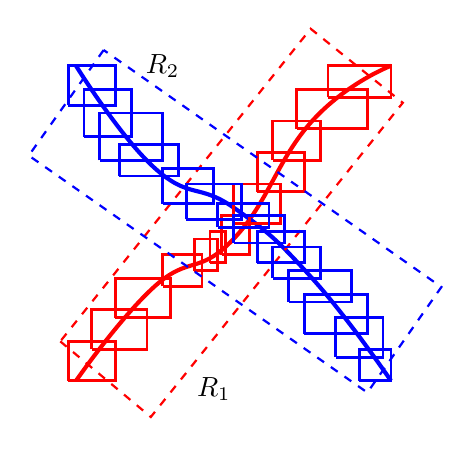
\begin{tikzpicture}

		\draw[color=red, line width = 1.5] plot[smooth, tension = .8] coordinates{
			(0, 0) (1, 1.2) (2, 1.8) (3, 3.3) (4, 4)
		};
		
		\draw[color=blue, line width = 1.5] plot[smooth, tension = .8] coordinates{
			(4, 0) (3, 1.3) (2, 2.2) (1, 2.7) (0, 4)
		};
		

		\draw[color = red, line width = 1] (-0.1, 0) -- (-0.1, 0.5) -- (0.5, 0.5) -- (0.5, 0) -- (-0.1, 0);
		\draw[color = red, line width = 1] (0.2, 0.4) -- (0.2, 0.9) -- (0.9, 0.9) -- (0.9, 0.4) -- (0.2, 0.4);
		\draw[color = red, line width = 1] (0.5, 0.8) -- (0.5, 1.3) -- (1.2, 1.3) -- (1.2, 0.8) -- (0.5, 0.8);
		\draw[color = red, line width = 1] (1.1, 1.2) -- (1.1, 1.6) -- (1.6, 1.6) -- (1.6, 1.2) -- (1.1, 1.2);
		\draw[color = red, line width = 1] (1.5, 1.4) -- (1.5, 1.8) -- (1.8, 1.8) -- (1.8, 1.4) -- (1.5, 1.4);
		\draw[color = red, line width = 1] (1.7, 1.5) -- (1.7, 1.9) -- (1.9,1.9) -- (1.9, 1.5) -- (1.7, 1.5);
		\draw[color = red, line width = 1] (1.85, 1.6) -- (1.85, 2.1) -- (2.2,2.1) -- (2.2, 1.6) -- (1.85, 1.6);
		\draw[color = red, line width = 1] (2.0, 2.0) -- (2.0, 2.5) -- (2.6, 2.5) -- (2.6, 2.0) -- (2.0, 2.0);
		\draw[color = red, line width = 1] (2.3, 2.4) -- (2.3, 2.9) -- (2.9, 2.9) -- (2.9, 2.4) -- (2.3, 2.4);
		\draw[color = red, line width = 1] (2.5, 2.8) -- (2.5, 3.3) -- (3.1, 3.3) -- (3.1, 2.8) -- (2.5, 2.8);
		\draw[color = red, line width = 1] (2.8, 3.2) -- (2.8, 3.7) -- (3.7, 3.7) -- (3.7, 3.2) -- (2.8, 3.2);
		\draw[color = red, line width = 1] (3.2, 3.6) -- (3.2, 4.) -- (4., 4.) -- (4., 3.6) -- (3.2, 3.6);
		
		\draw[color = red, line width = .8, dashed] (-0.2, 0.5) -- (0.95, -0.46) -- (4.15, 3.53) -- (2.98, 4.47) -- (-0.2, 0.5);

		\draw[color = blue, line width = 1] (3.6, 0) -- (3.6, 0.4) -- (4., 0.4) -- (4., 0) -- (3.6, 0);
		\draw[color = blue, line width = 1] (3.3, 0.3) -- (3.3, 0.8) -- (3.9, 0.8) -- (3.9, 0.3) -- (3.3, 0.3);
		\draw[color = blue, line width = 1] (2.9, 0.6) -- (2.9, 1.1) -- (3.7, 1.1) -- (3.7, 0.6) -- (2.9, 0.6);
		\draw[color = blue, line width = 1] (2.7, 1) -- (2.7, 1.4) -- (3.5, 1.4) -- (3.5, 1) -- (2.7, 1);
		\draw[color = blue, line width = 1] (2.5, 1.3) -- (2.5, 1.7) -- (3.1, 1.7) -- (3.1, 1.3) -- (2.5, 1.3);
		\draw[color = blue, line width = 1] (2.3, 1.5) -- (2.3, 1.9) -- (2.9, 1.9) -- (2.9, 1.5) -- (2.3, 1.5);
		\draw[color = blue, line width = 1] (2.0, 1.75) -- (2.0, 2.1) -- (2.65, 2.1) -- (2.65, 1.75) -- (2.0, 1.75);
		\draw[color = blue, line width = 1] (1.8, 1.95) -- (1.8, 2.25) -- (2.45, 2.25) -- (2.45, 1.95) -- (1.8, 1.95);
		\draw[color = blue, line width = 1] (1.4, 2.05) -- (1.4, 2.5) -- (2.1, 2.5) -- (2.1, 2.05) -- (1.4, 2.05);
		\draw[color = blue, line width = 1] (1.1, 2.25) -- (1.1, 2.7) -- (1.75, 2.7) -- (1.75, 2.25) -- (1.1, 2.25);
		\draw[color = blue, line width = 1] (.55, 2.6) -- (.55, 3.) -- (1.3, 3.) -- (1.3, 2.6) -- (.55, 2.6);
		\draw[color = blue, line width = 1] (.3, 2.8) -- (.3, 3.4) -- (1.1, 3.4) -- (1.1, 2.8) -- (.3, 2.8);
		\draw[color = blue, line width = 1] (.1, 3.1) -- (.1, 3.7) -- (0.7, 3.7) -- (0.7, 3.1) -- (.1, 3.1);
		\draw[color = blue, line width = 1] (-0.1, 3.5) -- (-0.1, 4) -- (0.5, 4) -- (0.5, 3.5) -- (-0.1, 3.5);
		
		\draw[color = blue, line width = .8, dashed] (0.351, 4.2) -- (-0.6, 2.86) -- (3.7, -0.15)-- (4.64, 1.19)  -- (0.351, 4.2);
		
		\node[label=below:] at (1.75, .-0.1) {$R_1$};
		\node[label=below:] at (1.1, 4.0) {$R_2$};
	\end{tikzpicture}
    % \includegraphics[width=0.5\linewidth]{curve_rotation.png}
    \caption{A schematic illustrating how self-intersections of the curves are detected.  The two rectangles contain the curve along their lengths and intersect on their lateral sides.  This guarantees a crossing of the curves.}
    \label{fig:crossing_rectangles}
\end{figure}

Before we begin the details of our test, we note that Algorithm \ref{algo:certified_curve_tracking} can be easily adapted to locally refine the tubular neighborhood $\cA(C)$.  Suppose that we wish to refine a consecutive sequence of tubes.  At each end of this sequence, there are points $x_1$ and $x_2$ that approximate the curve.  Without loss of generality, we assume that the direction in which we track $C$ passes $x_1$ first and then $x_2$.  By applying Algorithm \ref{algo:certified_curve_tracking} starting at $x_1$ and with small $\rho$ results in a refinement of the tubular neighborhood when the StoppingCriterion succeeds for the point $x_2$.




%\hrule


%\hrule




%We can exclude any intersections of the curve between these two regions 


%s until the approximation satisfies additional tests.  We provide an algorithm for constructing the tubular neighborhood of $\pi(C)$ and prove its correctness using some topological results.
 
%\begin{definition}
%    For a tubular neighborhood $\mathcal{A}(C)$ of a regular curve $C$, consider two interval tubes $I_1$ and $I_2$. We say that $I_1$ and $I_2$ are \emph{adjacent} if they are created consecutively by \Cref{algo:certified_curve_tracking}.
    
%    Furthermore, %we say that two interval tubes $I_1$ and $I_2$ \emph{intersect non-trivially} if $I_1\cap I_2\ne \emptyset$ and $I_1$ and $I_2$ are not adjacent. 
%    Finally, 
%if a generic projection $\pi:\mathbb{R}^n\rightarrow \mathbb{R}^2$ is given, we may define adjacency of $\pi(I_1)$ and $\pi(I_2)$ naturally.
%\end{definition}



%\begin{definition}
%    Let $C$ be a regular curve in $\mathbb{R}^n$ and $\pi:\mathbb{R}^n\rightarrow \mathbb{R}^2$ be a generic projection. For the projection $\pi(\mathcal{A}(C))=\{\pi(I_1),\dots, \pi(I_N)\}$ of the tubular neighborhood, we say that $\pi(I_i)$ is an \emph{intersecting tube} if there is $\pi(I_j)\in \pi(\mathcal{A}(C))$ intersecting non-trivially with $\pi(I_i)$.
%\end{definition}


% \begin{definition}
%     Let $\mathcal{A}_1$ and $\mathcal{A}_2$ be subcollections of $\mathcal{A}(C)$ such that each $\mathcal{A}_i$ consists of adjacent interval tubes.
%     We say that $\mathcal{A}_1$ and $\mathcal{A}_2$ \emph{intersect} if $I\cup\left(\bigcup_{J\in \mathcal{A}_2}J\right)\ne\emptyset$ for any $I\in \mathcal{A}_1$. In this case, we call $\{\mathcal{A}_1,\mathcal{A}_2\}$ an \emph{intersecting part}.
%     Furthermore, we say that $\mathcal{A}_1$ and $\mathcal{A}_2$ \emph{intersect transversally} if any deformation retract of $\bigcup_{I\in \mathcal{A}_i}I$ intersects transversally. 
% \end{definition}

% \textcolor{blue}{Sketch of the procedure.}
% \begin{itemize}
%     \item Build an adjacency list of all boxes in $\pi(\cA(C)).$
%     \item For each pair of intersecting boxes, $A$ and $B$ do the following:
%     \begin{itemize}
%         \item Test if the direction changes by more than $\pi$ radians. This is done by approximating the angle of the tangent vectors in each box between $A$ and $B$ inclusive. If the union of such angles covers more than half a circle (i.e., the angle changes by more than $\pi$ radians), then we refine. \textcolor{blue}{Do we refine just $A$ and $B$ or every box between too?}
%         \item If $\{A, B\}$ fail the $\pi$-test, then we move on to the strip test. To do this, we pick an arbitrary point in $ p \in A \cap B$ and compute the direction of the tangent vector for $\pi^{-1}(p) \in \pi^{-1}(A)$ and $\pi^{-1}(p) \in \pi^{-1}(B).$ Using the tangent vectors we construct tubes of radius \textcolor{blue}{something in terms of $\rho$ and $r$}. We then extend these two tubes until they are completely separated \textcolor{blue}{this distance can be determined with a little trig}. Extending outward from $A$ and $B$ through adjacent boxes, we check if a box intersects the ``walls'' of the tubes. If this type of intersection occurs, we refine. If the boxes ``escape'' the tubes through the end caps for both tubes, then we have an intersection. 
%         \item If we have detected an intersection using the strip test, we need to check for multiple intersections. To do this, we use the $C_1^\times$ test (\textcolor{blue}{this needs to be properly defined)}.
%     \end{itemize}
% \end{itemize}

% \begin{definition}
%     Let $\{\mathcal{A}_1, \mathcal{A}_2\}$ be an intersecting part of $\mathcal{A}(C)$. The \emph{intersecting completion} of $\{\mathcal{A}_1, \mathcal{A}_2\}$ is constructed as follows:
%     \begin{enumerate}
%     \item Add to $\mathcal{A}_2$ all interval tubes that intersect some $B \in \mathcal{A}_1$ but are not already adjacent to any $B \in \mathcal{A}_1$.
%     \item If $\mathcal{A}_2$ is no longer a contiguous collection of adjacent interval tubes, add the necessary adjacent interval tubes to restore contiguity.
%     \item Add to $\mathcal{A}_1$ all interval tubes that intersect some $B \in \mathcal{A}_2$ but are not already adjacent to any $B \in \mathcal{A}_2$.
%     \item If $\mathcal{A}_1$ is no longer a contiguous collection of adjacent interval tubes, add the necessary adjacent interval tubes to restore contiguity.
%     \item Repeat this process until no further interval tubes are added to either $\mathcal{A}_1$ or $\mathcal{A}_2$.
%     \end{enumerate} We say a pair $\{\cA_1, \cA_2\}$ is a \emph{complete intersecting part} if the intersecting completion of $\{\cA_1, \cA_2\}$ is the pair itself.
% \end{definition}

% How do we detect and remove regions where we suspect there may be multiple intersections?
% \begin{itemize}
%     \item Compute a tubular neighborhood $\mathcal{A}(C)$ of $C$.
%     \item For a generic projection $\pi$ consider $\pi(\mathcal{A}(C))$
%     \item Find all intersecting pairs $(\pi(\mathcal{A}_i),\pi(\mathcal{A}_j))$ from $\pi(\mathcal{A}(C))$. 
%     \item For intersecting $\pi(\mathcal{A}_1)$ and $\pi(\mathcal{A}_2)$, if they intersect transversally, then we conclude that there is no multiple intersections in the part. (need to prove. we may use the fact that the curve is contained ``uniquely'' in the tube.)
%     \item If there is a non-transversal intersection of $\pi(\mathcal{A}_1)$ and $\pi(\mathcal{A}_2)$, there must be deformation retract $r_i$ of $\pi(\mathcal{A}_i)$ such that $r_1$ and $r_2$ has  parallel tangent vectors. This will be detected via interval arithmetic as Michael wrote.
%     \item If $\pi(\mathcal{A}_1)$ and $\pi(\mathcal{A}_2)$ intersect non-transversally, we refine $\mathcal{A}_1$ and $\mathcal{A}_2$ further until non-transversal intersections are removed.
%     (we need to prove that a non-transversal intersection may be removed after sufficient refinements)
% \end{itemize}

%Let $C$ be a regular curve in $\RR^n$ with tubular neighborhood $\cA(C)$ and let $\pi:\RR^n \to \RR^2$ be a generic projection. Let $I_1$ and $I_2$ be two interval tubes of $\cA(C).$ We define $T_0(I_1, I_2)$ in the following way. First, we construct a sequence, $S,$ of adjacent interval tubes connecting $I_1$ and $I_2.$ If two such sequences exist, we consider both. For each interval tube $J_i \in S,$ we evaluate the Jacobian, $J_C(J),$ and compute its numerical kernel $K_i$ using interval arithmetic. Then, we consider $\pi(K_i)$ and determine the interval of angles of the tangent vectors of the curve. If the angle does not change by more than $\pi$ for at least one sequence $S,$ $T_0(I_1, I_2)$ returns $\true,$ otherwise $T_0(I_1, I_2)$ returns $ \false.$ 

%Let $C$ be a regular curve in $\RR^n$ with tubular neighborhood $\cA(C)$ and let $\pi:\RR^n \to \RR^2$ be a generic projection. Let $I_1$ and $I_2$ be two interval tubes of $\cA(C).$ We define the predicate $T_1(I_1, I_2)$ in the following way. We start by determining the Jacobian matrix, $J_C.$ Then, for each $I_i,$ we compute the numerical kernel $K_i.$ Then, we have $T_1(I_1, I_2) = \true$ when $0 \notin \pi(K_1) \times \pi(K_2),$ otherwise  $T_1(I_1, I_2) = \false.$ 

\begin{algorithm}[h]
	\caption{IntersectionCheck}
 \label{algo:strip_test}
\begin{algorithmic}[1]
\Require  
\begin{itemize}
    \item A regular curve $C=\{c_1,\dots,c_{n-1}\}\subset\mathbb{Q}[X_1,\dots,X_n]$
    \item A tubular neighborhood $\cA(C)$ obtained by Algorithm \ref{algo:certified_curve_tracking}
    \item A generic projection $\pi: \RR^n \to \RR^2$
    \item A pair of interval regions $\{I_1, I_2\}$ with intersecting projections
\end{itemize}
\Ensure 
\begin{itemize}
    \item A boolean value indicating confirmation of a self-intersection.
\end{itemize}
\State{Set $p$ to be the center of $\pi(I_1) \cap \pi(I_2)$}
\State{Construct approximation $v_i$ to the image of the tangent vector at $p$ for $\pi(I_i)$.}
\If{$v_1$ and $v_2$ are parallel}
\State{Refine $I_1$ and $I_2$}
\State{Return \false}
\EndIf
\State{Set $r$ to be the maximum diameter of $\pi(I_1)$ and $\pi(I_2)$.}
\State{Construct rectangular region $R_i$ to be a rectangle centered at $p$ whose width is of length $2r$ in the direction $v_i^\perp$ and whose length is long enough so that the edges of length $2r$ are outside the other rectangle.}
\State{Refine $\cA(C)$ until every interval region intersecting $R_i$ has diameter at most $r$.}
\State{Starting at $I_i$, find the first interval region in the forward and backward directions of $\cA(C)$ that are completely outside $R_i$.  Set $(F_i,L_i)$ to be these consecutive sequence of regions.}
\If{Either $(F_i,L_i)$ intersects the lateral sides of $R_i$}
\State{Refine all interval regions in $R_i$.}
\State{Return \false}
\EndIf
\If{Each $(F_i,L_i)$ does not satisfy the half-space tangent vector condition above}
\State{Refine all interval regions in $R_i$.}
\State{Return \false}
\EndIf
\For{{\bf each} pair of interval regions $J_i\in R_i$}
\State{Set $K_i$ to be an interval box containing the numerical kernel of $JC(J_i)$}
\If{$\pi(K_1)$ and $\pi(K_2)$ contain a parallel vector}
\State{Refine all interval regions in $R_i$.}
\State{Return \false}
\EndIf
\EndFor
\State{Return \true}
\end{algorithmic}
\end{algorithm}

% This algorithm was already started in algo:certified_plane_curve - Byrd Feb 5th

% \begin{algorithm}[ht]
% 	\caption{approximate plane curve from projection}
%  \label{algo:projection_approx}
% \begin{algorithmic}[1]
% \Require  
% \begin{itemize}
%     \item A regular curve defined by $n-1$ equations $C=(c_1,\dots, c_{n-1})$ in $\mathbb{R}^n$,
%     \item A tubular neighborhood $\cA(C)$ obtained by Algorithm \ref{algo:certified_curve_tracking}
%     \item A generic projection $\pi: \RR^n \to \RR^2$
% \end{itemize}
% \Ensure 
% \begin{itemize}
%     \item a refined $\cA(C)$ such that $\pi(\cA(C))$ is a tubular neighborhood of $\pi(C)$
% \end{itemize}
% \State{Initialize queue $Q$ containing all pairs of intersecting interval tubes $\{ I, J\}$ where $I, J \in \pi(\cA(C))$}
% \While{$Q$ is not empty}
% \State{pop pair $\{ I, J \}$ from $Q$} 
% \If{$T_0(I, J) = \false$}
% \State{refine $I$ and $J$ \textcolor{blue}{and every box in between?}}
% \State{update $Q$}
% \ElsIf{$I$ and $J$ fail the strip test}
% \State{refine all interval tubes contained in both strips}
% \State{update $Q$}
% \Else{}
% \State{accept $\{ I, J \}$}
% \EndIf
% \EndWhile
% \State{Return accepted regions.}
% \end{algorithmic}
% \end{algorithm}

We observe that if Algorithm~\ref{algo:strip_test} returns \true, then the curve must have a self-intersection, as described above.  In addition, if there were multiple intersections in $R_1\cap R_2$, then \cite[Lemma 3.1]{Byrd:2023} would imply that at the extreme point, i.e., when the curves are farthest apart, their tangent vectors would point in the same (or opposite) directions.  This is prevented by Line 21 of Algorithm~\ref{algo:strip_test}.  This implies that success of Algorithm~\ref{algo:strip_test} implies that there is exactly one intersection in $R_1\cap R_2$.  We now prove that after sufficient refinements both intersections and non-intersections can be detected, see Figure \ref{fig:two_projections}.

\begin{lemma}
    Let $C$ in $\RR^n$ be a regular curve and $\pi: \RR^n \to \RR^2$ a generic projection. Let $\cA(C)$ be the tubular neighborhood of $C$ constructed with Algorithm \ref{algo:certified_curve_tracking}. For every self-intersection of $\pi(C),$ there exists a pair of interval regions $I_1$ and $I_2$ such that Algorithm \ref{algo:strip_test} returns $\true$ after sufficient refinement.
\end{lemma}
\begin{proof}
Let $I_1$ and $I_2$ be the two interval regions such that there is a point $p_i\in I_i$ such that both $p_i$'s project to the same point.  When $I_1$ and $I_2$ are sufficiently small, $v_1$ and $v_2$ are approximately the tangent vectors of the projected curve at the intersection point.  Since all self-intersections are transversal, the tangent vectors at the intersection are not parallel, so, after sufficient refinement, $v_1$ and $v_2$ cannot be parallel either.

Since after sufficient refinement, the vectors $v_1$ and $v_2$ approach the tangent vectors of the projected self-intersection, the angles of the sides of $R_1$ and $R_2$ become stable, so the aspect ratio of each $R_i$ becomes nearly fixed.  Observe that any curve can be described locally by $p_0+tv_0+O(t^2)$.  For each branch at the self-intersection point $p\rightarrow p_0$ and, for some $i$, $v_i\rightarrow v_0$.  Finally, since the size of $R_i$ also gets smaller with refinement, the error in the curve is eventually small enough so that it passes through the ends of $R_i$ of length $2r$.  This implies that after sufficient refinement, $(F_i,L_i)$ cannot intersect the lateral sides of $R_i$.

Finally, by the same argument as above, after sufficient refinement, the tangent vector to the projected curve is nearly constant.  In addition, the calculated numerical kernels are also almost constant.  Therefore, after sufficient refinement, the tangent vectors are all pointing in almost the same direction, so the half-space tangent vector condition must hold.  Since the tangent vectors at the projected self-intersection are not parallel, this also implies that after sufficient refinement, the projected numerical kernels cannot contain parallel vectors.  

Therefore, after sufficient refinement, the IntersectionCheck algorithm returns \true.
\end{proof}



%In order to prove the correctness of Algorithm \ref{algo:certified_plane_curve}, we 


%provide the following lemmas.

%\begin{lemma}
%    Let $C$ in $\RR^n$ be a regular curve and $\pi: \RR^n \to \RR^2$ a generic projection. Let $\cA(C)$ be the tubular neighborhood of $C$ constructed with Algorithm \ref{algo:certified_curve_tracking}. For every self-intersection of $\pi(C),$ there exists a pair of intersecting interval tubes $\pi(I)$ and $\pi(J)$ in $\pi(\cA(C))$ such that Algorithm \ref{algo:strip_test} returns $\true$ after sufficient refinement.
%\end{lemma}

%\begin{proof}
    % Sketch
    % \begin{itemize}
    %     \item Start with the intersection point.
    %     \item Determine the smaller angle of tangent vectors at the intersection point
    %     \item Choose some distance $d$ for the length of the tubes in the direction of the tangents.
    %     \item Determine the radius of the tubes such that the ends of the tube do not intersect. This will depend on the angle of the tangents at intersection and the length of the tubes.
    % \end{itemize}
 %   Let $p$ be the point where $\pi(C)$ self intersections and define $p_I := \pi^{-1}(p) \in I$ and $p_J := \pi^{-1}(p) \in J.$ Construct straight tubes $T_I$ and $T_J$ directed and centered with the tangent of $C$ at $p_I$ and $p_J,$ respectively. Extend both $T_I$ and $T_J$ a distance of $d$ in both directions from $p_I$ and $p_J.$ Then, the radius of $T_I$ and $T_J$ is $\frac{d}{2}\tan\left(\frac{\theta}{2}\right),$ where $\theta$ is the angle between the two tangents of $\pi(C)$ at $p.$ As long as the interval tubes of $\pi(C)$ intersect the sides of $\pi(T_I)$ or $\pi(T_J),$ further refinement is required. To show that this process will terminate, we first show that there exists small enough tubes $T_I$ and $T_J$ such that $\pi(C)$ exits each through the ends. For small $d,$ we have that the curvature of $\pi(C)$ is approximately $O\left(d^2\right), $ therefore there exists $\tilde{d} > 0$ such that $T_I$ and $T_J$ have length $2\tilde{d}$ and radius $\frac{\tilde{d}}{2}\tan\left(\frac{\theta}{2}\right)$ and $\pi(C)$ exits $\pi(T_I)$ and $\pi(T_J)$ through the ends. It remains to show that the interval tubes approximating $\pi(C)$ do not intersect the sides of $\pi(T_I)$ or $\pi(T_J).$ Since $\pi(C)$ does not intersect the sides of $\pi(T_I)$ or $\pi(T_J),$ there is some positive $\tilde{r}$ that is the minimum distance from $\pi(C)$ to the sides of $\pi(T_I)$ and $\pi(T_J).$ Therefore, we can refine the interval tubes approximating $C$ within $T_I$ and $T_J$ such that the ``radius'' of each interval tube is less than $\tilde{r}$ after a finite number of steps.

    % \textcolor{blue}{Locally, a curve is of the form $p+tv+O(t^2)$.  Therefore, if the tube length is $\epsilon$, then the curve bends away from the midline by $O(\epsilon^2)$. If the side lengths of the tube are proportional, then the width of the tube is $O(\epsilon)$.  When epsilon is small, the curve must stay within the tube.}
%\end{proof} 

\begin{lemma}
    Let $C$ in $\RR^n$ be a regular curve and $\pi: \RR^n \to \RR^2$ a generic projection. Let $\cA(C)$ be a tubular neighborhood of $C$ constructed with Algorithm \ref{algo:certified_curve_tracking}.  If for two interval regions $I_1$ and $I_2$, $\pi(I_1)$ and $\pi(I_2)$ intersect but their curves do not correspond to a self-intersection, then this is detected after sufficient refinement.
\end{lemma}
    
%    do not correspond to a self-intersection, then 
    
    
%    If $T_0(I, J) = \false$ and $\pi(I)$ and $\pi(J)$ do not correspond to a self-intersection of $\pi(C),$ then $\pi(I) \cap \pi(C)$ and $\pi(J) \cap \pi(C)$ will be separated after sufficient refinement.
%\end{lemma}

\begin{proof}
    If there is a nonzero minimum distance between the images of the curves from $I_0$ and $I_1$, then once refinements of $I_0$ and $I_1$ have sufficiently small diameter, their projections will also have small diameter, and they cannot intersect.

    On the other hand, if the minimum distance is zero, this means that $I_1$ and $I_2$ correspond to a single arc of the curve.  After sufficiently many refinements, this portion of the arc is so small that the tangent vector does not change much over the arc and the half-space tangent vector condition succeeds.  In either case, the lack of an intersection is detected.
\end{proof}

    % Sketch
    % \begin{itemize}
    %     \item By assumption, we have that the subset of the projected curve does not intersect in $\pi(I) \cap \pi(J)$
    %     \item Define $C_I := \pi(I) \cap \pi(C)$ and $C_J := \pi(J) \cap \pi(C)$.
    %     \item Since $C_I \cap C_J = \emptyset$ and we are working over a compact region, we have that there is some positive infimum distance $m$ between $C_I$ and $C_J$. $m := \inf \{ \lVert x - y \rVert : x \in C_I, y \in C_J \} > 0.$ 
    %     \item Ensure that all interval tubes that are a result of some number of refinements of $I$ and $J$ have ``radius'' smaller than $m/2$. 
    % \end{itemize}
    
%    Let $C_I := \pi(I) \cap \pi(C)$ and $C_J := \pi(J) \cap \pi(C).$ By assumption, we have that $C_I$ and $C_J$ do not intersect. Let $m = \inf \{ \lVert x - y \rVert : x \in C_I, y \in C_J \} > 0. $ It suffices to show that, after sufficient refinement, the distance between $C_I$ and the interval tubes containing $C_I$ is less than $m/2.$  We have for any interval tube $\tilde{I} \in \cA(C),$ \[d(C \cap \tilde{I}, \tilde{I}) := \sup_{x \in C \cap \tilde{I}} \inf_{a \in \partial \tilde{I}}\{ \lVert x - a\rVert \} \leq \rho \cdot r, \] where \textcolor{blue}{``explanation regarding $\rho$-approximations.''} Moreover, we have that $d(\pi(C \cap \tilde{I}), \pi(\tilde{I})) \leq d(C \cap \tilde{I}, \tilde{I}).$ Therefore,  every interval tube, $\tilde{I},$ containing $C_I$ can be refined such that $d(C_I, \tilde{I}) < \frac{m}{2}$ after finitely many steps. Similarly, we can show the same is true for $C_J.$ Therefore, we have that $\pi(I) \cap \pi(C)$ and $\pi(J) \cap \pi(C)$ can be separated after sufficient refinement.
%\end{proof}

Putting these lemmas together, we have the following theorem.

\begin{thm}
    Let $\pi:\mathbb{R}^n\rightarrow\mathbb{R}^2$ be a generic projection. For a regular curve $C$ in $\mathbb{R}^n$, Algorithm \ref{algo:certified_plane_curve} returns a tubular neighborhood $\mathcal{A}(C)$ of $C$ such that $\pi(\mathcal{A}(C))$ is a tubular neighborhood of $\pi(C)$. 
\end{thm}
\begin{proof}
We must only argue that in Algorithm \ref{algo:certified_plane_curve}, no intersection is detected twice.  To see this, suppose that an intersection is detected twice.  In this case, since the rectangles $R_i$ for each test of Algorithm \ref{algo:strip_test} separate the approximations and separate the arcs of the projected curves, the two pairs of boxes must be contained in each other's $R_i$'s, which is not possible by Line 13 of Algorithm \ref{algo:certified_plane_curve}.  
\end{proof}

\begin{thm}
    \Cref{algo:certified_plane_curve} terminates within finitely many iterations.
\end{thm}


% Let $C$ be a regular curve defined by $n-1$ equations $(c_1, \ldots, c_n)$ in $n$ dimensional space. We start by computing a tubular neighborhood $\mathcal{A}(C)$ using Algorithm NUMBER. Then, we consider the projection $\pi\left( \mathcal{A}\left( C \right) \right),$ where $\pi$ is a generic projection. Consider the following procedure. Let $\mathcal{Q}$ be a queue of all pairs $\left( \pi\left( \mathcal{A}_i \right), \pi\left( \mathcal{A}_j \right) \right)$ such that $\pi \left(\mathcal{A}_i\right) \subseteq \pi\left( \mathcal{A}\left( C \right) \right), i \neq j,$ and $\pi\left( \mathcal{A}_i \right) $ and $ \pi\left( \mathcal{A}_j \right)$ intersect. For each pair in $\mathcal{Q},$ such that $\pi\left( \mathcal{A}_i \right) $ and $ \pi\left( \mathcal{A}_j \right)$ intersect transversally, we have that the corresponding curves of \textcolor{blue}{to be continued...}

% We are not dealing with intersecting parts anymore - Byrd Feb 5th

% \begin{algorithm}[ht]
% 	\caption{removing non-transversal intersecting part}
%  \label{algo:remove_non_transversality}
% \begin{algorithmic}[1]
% \Require  
% \begin{itemize}
%     \item A regular curve defined by $n-1$ equations $C=(c_1,\dots, c_{n-1})$ in $\mathbb{R}^n$,
%     \item A non-transversally intersecting part $\{\mathcal{A}_1,\mathcal{A}_2\}$.
%     \item A constant $\tau\in (0,1/2]$.
% \end{itemize}
% \Ensure 
% \begin{itemize}
%     \item a refined $\mathcal{A}_1$ and $\mathcal{A}_2$ that are intersecting transversally, or disjoint.
% \end{itemize}

% \State{Enumerate  $\mathcal{A}_1=\{I_1,\dots, I_N\}$.}
% \For{$I\in \mathcal{A}_1$}
% \State{Define $\mathcal{I}:=\{J\in \mathcal{A}_2\mid I\cap J\ne \emptyset\}$.}
% \State{Compute the tangent vector $r'(I)=\begin{bmatrix}
%     A^{-1}(I)\mathbf{v}(I) \\
%     1
% \end{bmatrix}$ for $I$ and all $J\in \mathcal{I}$.}
% \While{$r'(I)$ is parallel to $r'(J)$ for some $J\in \mathcal{I}$}
% \State{Redefine $\tau=\frac{\tau}{2}$.}
% \State{Refine $I$ and $J$ with $\tau$.}
% \State{Whenever new interval tubes $\{I_{i_1},\dots, I_{i_k}\}$ created from refining $I$, redefine $\mathcal{A}_1:=\mathcal{A}_1\cup \{I_{i_1},\dots, I_{i_k}\}$.}
% \State{Whenever new interval tubes $\{J_{j_1},\dots, J_{j_k}\}$ created from refining $J$, redefine $\mathcal{A}_2:=\mathcal{A}_2\cup \{J_{j_1},\dots, J_{j_k}\}$.}
% \State{\color{blue} TODO: prove that refining boxes sufficiently removes parallel tubes.}
% \EndWhile
% \EndFor
% \State{Return $\mathcal{A}_1$ and $\mathcal{A}_2$.}
%  \end{algorithmic}
%  \end{algorithm}


\begin{algorithm}[ht]
	\caption{CertifiedPlaneCurve}
 \label{algo:certified_plane_curve}
\begin{algorithmic}[1]
\Require  
\begin{itemize}
    A regular curve $C=\{c_1,\dots,c_{n-1}\}\subset\mathbb{Q}[X_1,\dots,X_n]$,
    \item a point $x$ approximating a nonsingular point on the curve $C$,
    \item a positive number $r>0$ for the initial radius.
    \item a generic projection $\pi:\mathbb{R}^n\rightarrow \mathbb{R}^2$,
    \item a compact region $D$,
    \item constants $\rho\in(0,\frac{1}{2}]$ and $\tau\in(\frac{1}{2},1)$.
\end{itemize}
\Ensure 
\begin{itemize}
    \item a certified tubular neighborhood of a plane curve $\pi(C)$.
\end{itemize}

\State{Compute a tubular neighborhood $\mathcal{A}(C)$ of $C$ using Algorithm $\ref{algo:certified_curve_tracking}$ with $C, x, r, D$, $\tau$, and $\rho$.}
% \State{For a generic projection $\pi$ consider $\pi(\mathcal{A}(C))$}
% \State{Find all intersecting parts from $\pi(\mathcal{A}(C))$.}
\State{Initialize queue $Q$ containing all pairs of intersecting interval regions $\{ I_1,I_2\}$}
\While{$Q$ is not empty}
\State{Pop pair $\{ I_1, I_2\}$ from $Q$} 
\If{$I_1$ and $I_2$ satisfy the half-space tangent vector condition}
\State{Accept $I_1$ and $I_2$}
\State{Do not consider $I_1$ and $I_2$ or their children as a pair again.}
\ElsIf{Algorithm \ref{algo:strip_test} on $I_1$ and $I_2$ returns $\false$}
\State{Refine the interval regions as described in Algorithm \ref{algo:strip_test}.}
\State{Update $Q$ with all pairs of intersecting interval tubes}
\Else{}
\State{Accept $I_1$ and $I_2$}
\State{Discard all other pairs $J_1\subset R_1$ and $J_2\subset R_2$ in $Q$ where $R_1$ and $R_2$ are the regions computed in Algorithm \ref{algo:strip_test}.}
\EndIf
\EndWhile
\State{Return accepted regions.}
 \end{algorithmic}
 \end{algorithm}

 In addition, if we wish to create an approximation to the projection to the curve itself, we may take the projection of the curve constructed in $\mathbb{R}^n$, with care to remove all self-intersections except those indicated by Algorithm \ref{algo:strip_test}.

 \begin{remark}
If the curve $C$ is not closed and is given by a parametric curve $C=\gamma(t)$.  Then, we may turn this into an implicit system by increasing the dimension by $1$ and considering the system of polynomials $X_i-\gamma_i(T)$.  In this case, we are interested in projections that include the $T$-direction in their kernel.  If such a projection is generic, then Algorithm \ref{algo:certified_plane_curve} correctly approximates the projection, see Figure \ref{fig:PTOPO_example}.
 \end{remark}
